%% $RCSfile: proj_report_outline.tex,v $
%% $Revision: 1.2 $
%% $Date: 2010/04/23 02:40:16 $
%% $Author: kevin $

\documentclass[11pt
              , a4paper
              , twoside
              , openright
              ]{report}


\usepackage{float} % lets you have non-floating floats

\usepackage{url} % for typesetting urls

\usepackage{graphicx} %I have some pictures :3

%
%  We don't want figures to float so we define
%
\newfloat{fig}{thp}{lof}[chapter]
\floatname{fig}{Figure}

%% These are standard LaTeX definitions for the document
%%                            
\title{Reputation Scraper - Social Media}
\author{Iain Walker}

%% This file can be used for creating a wide range of reports
%%  across various Schools
%%
%% Set up some things, mostly for the front page, for your specific document
%
% Current options are:
% [ecs|msor]              Which school you are in.
%
% [bschonscomp|mcompsci]  Which degree you are doing
%                          You can also specify any other degree by name
%                          (see below)
% [font|image]            Use a font or an image for the VUW logo
%                          The font option will only work on ECS systems
%
\usepackage[font,ecs,mcompsci]{vuwproject}

% You should specifiy your supervisor here with
     \supervisor{Kris Bubendorfer}
% use \supervisors if there is more than one supervisor

% Unless you've used the bschonscomp or mcompsci
%  options above use
\otherdegree{ENGR489 - Bachelor of Engineering}
% here to specify degree

% Comment this out if you want the date printed.
\date{}

\begin{document}

% Make the page numbering roman, until after the contents, etc.
\frontmatter

%%%%%%%%%%%%%%%%%%%%%%%%%%%%%%%%%%%%%%%%%%%%%%%%%%%%%%%

%%%%%%%%%%%%%%%%%%%%%%%%%%%%%%%%%%%%%%%%%%%%%%%%%%%%%%%

\begin{abstract}

Online reputation has become increasingly important as more social and business interactions move online. This project is concerned with investigating how we can infer basic reputation metrics from non-traditional sources such as social media sites, including Facebook, Twitter, Google+, LinkedIn, and Slashdot. The method of gathering has been through web-scraping, since most social media sites do not (understandably) have an API to retrieve this information without logging in to the system. The project has looked at developing web-scrapers to retrieve publicly-available information on social media sites, and investigating how this can be used to infer basic reputation metrics. 

\end{abstract}

%%%%%%%%%%%%%%%%%%%%%%%%%%%%%%%%%%%%%%%%%%%%%%%%%%%%%%%

\maketitle

%%%\chapter*{Acknowledgements}

I would like to thank my supervisor Kris Bubendorfer who was endlessly free with his experience and advice.  

\tableofcontents

% we want a list of the figures we defined
\listof{fig}{Figures}

%%%%%%%%%%%%%%%%%%%%%%%%%%%%%%%%%%%%%%%%%%%%%%%%%%%%%%%

\mainmatter

%%%%%%%%%%%%%%%%%%%%%%%%%%%%%%%%%%%%%%%%%%%%%%%%%%%%%%%

% individual chapters included here
\chapter{Introduction}\label{C:int}

Social Networking Sites (SNS) such as \textit{theFacebook} originated in University environments in the early 21st century. Users on social sites are able to create profiles about themselves, and interact with other users. The size of social networking services has grown exponentially with 1.05 billion monthly users on Facebook in December 2012 \cite{fb_users}. Online social platforms such as Facebook, Twitter, Google+ and LinkedIn have served to largely complement real-life interaction. Interactions online may take place with a variety of social spheres; friends, co-workers, family and complete strangers all congregate in one online location \cite{johnson2012facebook}. As these social and business transactions move online, defining who we should and should not trust becomes increasingly important, yet hard to resolve. Although SNS to some extent have inbuilt concepts of trust, using contact networks (Facebook, LinkedIn) and circles (Google+) for example, the concept of trustworthiness is more blurred. Tools to provide a snapshot or hint of an individual's reputation and trustworthiness could be useful. 

% In the digital age many social and business transactions are moving online. As such, defining who we should and should not trust becomes increasingly important, yet hard to resolve. Although SNS to some extent have inbuilt concepts of trust, using contact networks (Facebook, LinkedIn) and circles (Google+) for example, the concept of trustworthiness is more blurred. Tools to provide a snapshot, or hint of an individual's reputation and trustworthiness could be useful. 

Reputation and the task of maintaining one's online reputation is a task often discussed, but with few metrics associated as to what defines an online reputation, or how to evaluate reputation online. Evaluating the standing of users in other communities has been useful for describing access rights \cite{graft_paper}, filtering spam and low quality posts \cite{josang2007survey}, and evaluating the likely quality of feedback on Question and Answer websites \cite{movshovitzanalysis}. This challenge of defining and quantifying reputation was a fundamental motivation for the project.

% This provided a fundamental drive to the project.

% In traditional networking terminology, reputation is a global trust mechanism, as opposed to trust which describes one nodes impression of another in the network. 

% Redo this second paragraph.

% which should influence other members of the networks opinions on the node. 

% Paragraph about social media and how social media has expanded into wide use.

% Paragraph about concepts of reputation. 

% Give a real introduction to the problem domain. What is social media and what is reputation, etc. 

\section{Motivation}

Reputation systems on trading websites have been extremely successful, despite the potential for fraudulent activity \cite{resnick2002trust}. While we might expect a self-aware adult to fairly easily spot equivalent 'fraudulent' activity or deceptive behaviour on social media, many examples have shown this to be untrue. Social crowd sourcing gone wrong has also been a high-profile issue, with incidents such as the Boston Bombings \cite{crowdsourcing_wad,doan2011crowdsourcing,brabham2008crowdsourcing}.

Various strategies have been used to infer the personality or active traits of individuals online; these have been shown to be highly accurate. Applications on SNS have been used to give people an idea of their own personality. The results can then be compared against elements of the person's use of social media. This requires the express permission of the individual concerned to gain any meaningful data, when collecting information through a site's API. While privacy concerns must be taken into account, publicly available information on an individual or company's social media account can be considered fair game. This information could be useful when judging trustworthiness. A new approach, that does not need permission to access information which is publicly-available is needed. 

\section{Proposed Solution}
A solution to the above issues is to use web-scraping strategies to anonymously retrieve reputation data. A more traditional approach would be to retrieve information directly through an API, but few social networks provide sufficient APIs - and they all require express user permission to work. This new system could be used to calculate a person's standing in a community. 

% This system could be used to give a general snapshot about an individual, by using these non-traditional data sources. There are many potential applications and uses for this sort of application.

The aim of this project is to demonstrate the feasibility of a tool that gathers and provides snapshot reputation data from social media sites, using web-scraping as the data gathering method. A framework for scraping social media sites is created called IHPScrape, and is applied to case studies of Twitter, Facebook and LinkedIn. A Twitter dataset is gathered of 1.7 million tweets. Access policies are written based upon the calculated standing of individuals in the community. The Twitter dataset was rich in semantic potential for analysis, and multiple approaches are taken to structure these policies. Retweet and favourite numbers, temporal clustering and community detection are the avenues explored for reputation calculation. 

% Access policies were written based upon the calculated standing of individuals in the community.

% This dataset was found to be rich in semantic potential for analysis, and multiple approaches were taken to structure these policies. 

% By creating such a reputation scraper, we envisage that a general impression about an individual on social media may be constructed. I create a new framework for scraping social media sites called IHPScrape, with the case study of Twitter, Facebook and LinkedIn as examples of the framework's applicability. A Twitter dataset is gathered of 1.7 million tweets, from which reputation metrics and policies are discussed. Finally I evaluate the performance and accuracy of this framework and reputation policies to analyse their potential effectiveness in a larger system.

\section{Contributions}
The primary contributions of this project are:

\begin{description}
	\item [A web-scraper for Twitter] as part of a wider scraping framework. Existing Twitter scrapers exist, but with performance and usage limitations that are unsuitable for fetching large quantities of data, or indeed reputation-focused data.
	
	\item [A web-scraping framework] that is suitable for extension onto more social networking sites is created called IHPScrape. The framework abstracts low-level networking details for further works, and reduces development time.
	
	\item [A dataset of 1.7 million tweets,] and associated tweet meta-data is created. This dataset was randomly selected. Existing Twitter datasets that were found online were predominantly celebrity based and not useful for research purposes. 
	
	\item [A set of reputation-inferring policies] for use on Twitter are described, with the potential for more to be created. These exemplar policies are created with reference to observed patterns in collected data.
	
	\item[Identification of a Strong Correlation] between Retweet and Favourite counts. This correlation is used as the basis for further policies, by showing that use of retweets and favourites is equivalent for measurement of user impact.
	
	\item [A Twitter Impact Factor] that describes a Twitter user's standing in the community as a function of retweet counts. This builds upon the Hirsch-Index \cite{hirsch2005index} calculation of an academic's standing in the community.
	
		
\end{description}

\section{Report Structure}

The remainder of the report is organised as follows. Chapter 2 summarises background work. Software engineering methodologies used throughout the project are described in Chapter 3, followed by the identified requirements in Chapter 4. Chapter 5 describes the design and implementation of the web scraping framework. Data collected using this framework is covered in Chapter 6. Chapter 7 then evaluates the scraping framework created. Finally, Chapter 8 provides conclusions and future work.

% The remainder of the report is structured as follows. Chapter 2 summarises background research that was undertaken in the problem domain. Chapter 3 describes the software engineering methodology used throughout the project. Chapter 4 identifies the specific requirements that the project aims to meet. Chapter 5 describes the design and implementation of the web scraping framework. Chapter 6 analyses data collected and proposes exemplar policies to determine social reputation. Chapter 7 then evaluates the scraping framework created. Chapter 8 provides conclusions and future work.

%The major contribution of the project is to deliver a prototype that gathers online reputation data using web-scraping techniques.The prototype will be integrated with the GRAft reputation system \cite{graft_paper}, in order to link with a person's OpenID\cite{open_id}. Users would be able to generate a reputation value for themselves, or for others they know. 
%explain below sentence!
%It aims to investigate alternative reputation sources, and look at how these can be applied in a practical sense. 

%Provide a scraping framework
%Provide a well-developed and tested scraper for twitter
%Provide a set of reputation policies
%Provide a dataset of 1.7 million tweets, and associated meta-data.
\chapter{Background}\label{C:us}

%What background is there into the research domain

%Web-scraping background and concepts

%Social media personality analysis

%Social media behaviour analysis, showing that social media actions correspond to individuals real-life actions to some respect

%Classification and dynamic access-driven policies, could these potentially be applied to social media

%Quantifying reputation on social media - what this means. Examples of systems that attempt to quantify reputation on social media, through the use of APIs and how a system I build could extend upon these. 

This section covers the background research I performed for the project, and works related to my project. I also discuss how I was able to contribute to the research domain, with points of difference to these works. 

\section{Social Media}

Social Networking Sites (SNS) have achieved massive adoption and user numbers since their inception. SNS describes any web site that enables users to create public profiles and form relationships with others. The SNS market has largely stabilised, with Facebook achieving market dominance. When deciding which sites to fetch data from, research was conducted into the most popular SNS, and features that could be applied into some reputation score. In order to fetch useful information, various social media sites were investigated in the context of gathering reputation data, and seeing what could be selected.

% In order to fetch useful information, I looked at the various social media sites in the context of gathering reputation data, and seeing what could be selected. 


%Insert diagram of the social networking market share. 

%Social Media Sites (SNS) 

%A background to social media. What defines a social media site. 

%What are social media sites

%What sites did I scrape, what was I able to do

%Web scraping was the technique used, discuss this next.

%Until now, the reasoning behind my social media selection has been largely neglected. In order to gather useful data, I looked at the various social media sites in the context of gathering reputation data, and seeing what could be fetched. %Add to this. Not very good currently... 


\begin{itemize}

\item Facebook \cite{facebook_site}: Publicly available information on Facebook includes data such as a user's Likes, Posts to Walls, and Friend networks. 
\item LinkedIn \cite{linkedin_site}: The primary business social network on which professionals can display information pertaining to their career and skills. Reputation data is fairly concrete - endorsements, skills, groups, and recommendations. 
\item Twitter \cite{twitter_site}: A SNS allowing posts of up to 140 characters. Information available includes number of followers, number of profiles the person is following, number of posts, and post data itself. Post data includes retweet and favourite count, the content itself, as well as the people who retweeted the tweet itself. 
\item Google+ \cite{google_site}: Similar to Facebook in style, and holds a large user base, but with much lower daily use than Facebook.
\item Slashdot \cite{slashdot_site}: A social media and news network targeted at a 'geek' audience. Slashdot is one of few social media sites that uses a positive/negative rating system on posts. This inbuilt reputation system could be interesting to look at further, when porting data between social media platforms. It is also unique from the standpoint of identifying 'trolls' - for which the website is widely known. 
\end{itemize}

This basic feature analysis was the foundation for data exploration on the social media sites scraped. As the project's primary aim was to demonstrate the fesibility of web-scraping as a means for fetching such information, research was conducted on web-scraping as a technology. 

\section{Web-Scraping}

% Web-scraping or \textit{screen scraping} refers to the practice of downloading web pages directly through HTTP requests, and parsing this unstructured data into something useful. It is a wel-understood data-gathering technique, and there are existing architectures and frameworks to help facilitate this. Anything online that is accessible through a browser can be scraped. 

Web-scraping or \textit{screen scraping} refers to the practice of downloading web pages directly through HTTP requests, and parsing this unstructured data into something useful. It is a well-understood data-gathering technique, and there are existing architectures and frameworks to help facilitate this.  Anything online that is accessible through a browser can be scraped. Hartley gives a light introduction to the concepts and strengths of web-scraping \cite{no_api_for_me}. Web-scraping is largely used as an alternative to traditional API's to websites, where these may not exist, or face a lack of support or development. Applications using web-APIs which frequently change could also benefit from switching to a web-scraping alternative. The advantage of web-scraping is that it provides direct access to the content of a website. While a site's API may not allow access to information that is quite clear from the front end, web-scraping will inherently provide this. Also, some sites do not monitor their API status 
as carefully as the actual front-end access. Maintaining availability to the core site is of higher business priority than developer APIs, and this is consistently reflected in respective levels of support. 

The primary limitation of web-scrapers is that major user interface changes will likely result in a broken scraper. In general site's structures do not change frequently enough for this to be a major issue. The typical argument however is that a site's structure can, without any warning, change at any time. This is an unavoidable issue when considering developing a scraper, and as such the regularity of user interface changes on a website should be considered when deciding between using an API or a scraper. In general it is more sensible to inspect a site's API for applicability before constructing a web-scraper. As an example; Facebook was ruled out as a social option in this project due to its regular user interface updates. 

However these interface change limitations can also be applied to modern social media APIs. Past projects fetching data from Facebook have had difficulty maintaining applications due to its too-often changed API \cite{kosinski2013private}. In the course of this project, Twitter's API changed such that the possibility of fetching required data through this interface was rendered infeasible. When considering scraping data, legal and privacy considerations must also be applied.

%Limitations of scrapers
%Although web-scrapers tend to break when user interfaces change, in general sites structures do not change frequently enough for this to be a major issue. However they can, without any warning, change at any time which limits web-scraping as a technology. Keep in mind that most websites do not change so frequently as for this to be an issue, although it did rule out Facebook as a candidate for my project. 

%A counter to the limitations of web-scrapers is the frequency of API changes on modern social media sites. Past projects fetching data from Facebook have failed due to its too-often changed API \cite{}. In the course of this project, Twitter's API changed such that the possibility of fetching required data through this interface was rendered infeasible. When considering scraping data, legal and privacy considerations must also be applied.

%Look at some applications of web-scraping.

%Web scraping vs APIs?

\subsection{Legal and Privacy Issues}

Companies such as Google and Facebook are widely known to use web-scraping on SNS and other sites for the purposes of web-indexing and advertising \cite{no_api_for_me}. Despite this, other entities attempting to commercialise such aggregated data have been met with threats of hostile law action. Pete Warden discusses how his data-mining experiences on Facebook nearly resulted in legal action \cite{facebook_sued}. In these cases, though, data-mining was intended to be used for commercial purposes. 

As an academic project, fears of legal retaliation are much lower. However strategies were enforced in order to stay within the terms of service of social sites. By never signing into the SNS that I retrieve data from, I inherently do not agree to the user terms of service\footnote{https://twitter.com/tos}. I also followed general positive web-scraping practices where possible, in order to limit possible negative effects of my scrapers upon these sites. Examples include attempting to adhere to a sites robots.txt, and the placement of reasonable pauses between requests to reduce server burden. 

\section{Inferring Information from Social Media}

The following sections examine research conducted into what information has already been investigated on social media. In particular, private personality traits that are inferrable from publicly available data are discussed, as well as how sentiment analysis of SNS can predict unexpected variables. 

% I now examine research conducted into what information has already been investigated on social media. In particular I discuss what private personality traits are inferrable from publicly available data, as well as how sentiment analysis of SNS can predict unexpected variables.
%In particular what private personality traits can be inferred from publicly-available data, as well as 

%Discuss the core challenges of web scraping in a social media setting

\subsection{Personality from Social Media}

Studies have investigated how private details about personality traits can be inferred through behavioural analysis of individuals on social media \cite{adali2012predicting,adali2012actions,bachrach2012personality,golbeck2011predicting,golbeck2011computing,golbeck2011,golbeck2011experimental}. Golbeck et al. demonstrate that real life personality traits may be predicted by looking at past behavioural patterns on Twitter with high accuracy \cite{golbeck2011predicting}. Using the publicly-available figures of followers, following and posts the authors were able to classify individuals into different Big Five personality types \cite{de2000big}. This was verified against a 44-question personality test for 71 individuals, with accuracy of around 80\%. In further papers these authors were also able to make conclusions on political preference, as well as extend their work onto Facebook and tagging behaviour \cite{golbeck2011computing,golbeck2011,golbeck2011experimental}. Adali et al. \cite{adali2012predicting,adali2012actions} extend this work further by predicting personality and relationship information on Facebook.
%Sentiment-based analysis of tweets has also been studied, analysing the use of emoticons on Twitter.
%Studies have shown how private details about personality traits can be inferred by behavioural analysis of individuals on social media. These studies have taken both a behavioural-based and textual sentiment-analysis approach to determine personality. Studies showed that real life personality traits can be predicted by looking at past behavioural patterns on Twitter, with high accuracy \cite{}. Using publicly-available information on Twitter pages, the authors were able to classify individuals into different Big-Five personality types \cite{}. This was verified against a 44-question personality test for 71 individuals, with accuracy of around 80\%. Further research has been performed, looking at how Facebook behavioural patterns relate to personality type by asking questions on the MyPersonality Facebook app. Behavioural data was then gathered from the test subject's Facebook profiles, to check for correlations. Textual sentiment-analysis approaches have also been taken in order to determine personality 
% type 
%from social media profiles. Sentiment-based analysis of tweets has also been studied, analysing the use of emoticons on Twitter \cite{kewalramanisentiment}.

While these studies showed how private personality details can be inferred from publicly-available data, they were made using applications which had to be given express permissions to access this data. In other words, although the conclusions drawn from these papers was that massive data-mining could be undertaken on these profiles as all the data is publicly available, they never used an approach that demonstrated the true feasibility of this. Clearly as social media site API's are properly locked-down and require authorisation of the relevant users to retrieve data\footnote{https://developers.facebook.com/docs/reference/apis/}, a web-scraping approach must be used. Such an approach allows applications to only require the same permissions as any human being accessing the same page, whilst also allowing the same data to be downloaded and aggregated.

A potential weakness in these studies is that personality on SNS may not translate well into actual personality. Although this may seem like a logical conclusion (e.g. Trolls, shallow internet relationships), studies have shown it to be false. Quercia et. al. demonstrated how popular Facebook users in fact maintain meaningful relationships with their hundreds of friends, and not the superficial ones we may expect \cite{quercia2012personality}. Again the Big Five personality model was used, and verified against popular Facebook users who used the MyPersonality app. Back et. al. demonstrated how Facebook profiles in fact are reflective of actual personality, and not a self-idealisation \cite{back2010facebook}. This study used manual inspection of profiles to make first impressions of individuals, which were compared against results from a Big Five personality test. Making similar predictions with computers would be an interesting and difficult challenge. 

\subsection{Sentiment and Temporal Information from Social Media}

It is also possible to take sentiment and temporal-related information from social sites as a whole, and use trending information to make accurate predictions about seemingly unlinked occurances. Bollen et al. \cite{bollen2011twitter} demonstrated that the 'mood' of Twitter can be used as a predictor of the U.S. stock market. The authors argue that Twitter mood is an accurate predictor of the public's mood state in general, which affects human decision-making and as such financial decisions. By taking historical Twitter data and calculating mood values using a classifier, the authors showed that Twitter was an accurate predictor of the U.S. stockmarket.

In a similar temporal approach to social BigData analysis, Ginsberg et al. \cite{ginsberg2008detecting} investigate detecting influenza epidemics using Google search query data. By analysing the relative frequency of certain queries implying health information-seeking online, early predictions and detection of epidemics may be possible. These examples demonstrate that information that may be thought of as seperate can be determined from the wealth of information on social media.

%Talk about research conducted into social media, with respect to temporal analysis and predicting stock markets, etc.

%Various temporal-clustering and sentiment based analysis studies have been conducted on social media. Bollen et al \cite{} demonstrated that the 'mood' of Twitter can determine the U.S. stock market. 
\section{Quantifying Reputation on Social Media}

% The above studies demonstrate how private personality and public 

Although the above studies investigate the concept of personality and how we can quantify this using social media, they did not expressly address the concept of reputation. Therefore we should discuss what reputation explicitly means on social media, and how sites currently help express user reputation. 

Some sites explicitly reference user reputation, a system commonly utilised on social forums. Stack Overflow \cite{stackoverflow_site} is a question and answer site where users are able to post code-related programming problems. It has been identified that sites such as Stack Overflow are largely dependant on the contributions of a small number of expert users, who provide a significant proportion of useful answers \cite{movshovitzanalysis}. As such, identifying users who have the potential to become strong contributors is of significant importance to the success of the website.

\begin{figure}[h!]
\begin{center}
\begin{tabular}{l|r}
 Action & Reputation Change\\ \hline
 Answer is voted up & +10 \\
 Question is voted up & +5 \\
 Answer is accepted & +15 (+2 to acceptor) \\
 Question is voted down & -2 \\
 Answer is voted down & -2 (-1 to voter) \\
 Experienced Stack Exchange user & onetime + 100 \\
 Accepted answer to bounty & +bounty \\
 Offer bounty to question & -bounty \\ 
\end{tabular}
%Actions and Corresponding Reputation Change on Stack Overflow \cite{movshovitzanalysis}
\end{center}
\caption{Actions and Corresponding Reputation Change on Stack Overflow \cite{movshovitzanalysis}}
\end{figure}

%Actions and Corresponding Reputation Change on Stack Overflow \cite{movshovitzanalysis}\\

%\caption{Actions and Reputation Change on Stack Overflow\cite{movshovitzanalysis}}\\

Reputation in this context is entirely derivative of the actions and effectiveness of answers provided by users. Within Stack Overflow, a high user reputation score could be considered a measure of expertise.

The online forum SlashDot \cite{slashdot_site} is another social site where user action affects reputation. Slashdot was created in 1997 as a 'news for nerds' message board \cite{josang2007survey}. As members grew rapidly, spam and poor posts became an issue, resulting in the introduction of a moderation system. A two tier moderation system now exists, where \textit{M1} allows administration of comments on articles, and \textit{M2} moderating the \textit{M1} moderators. User reputation information is logged using \textit{Karma} for logged in users as a reputation metric. Each logged in user maintains a \textit{Karma} score from one of six discrete values: \textit{Terrible, Bad, Neutral, Positive, Good, Excellent}. Positive moderation feedback to a user's comment will result in an increase in Karma. The opposite applies for negative moderation. Comments on SlashDot are ranked from [-1,5]. If a user with high Karma created a comment, this will have a higher starting rank. To reduce spam, users 
can then filter comments based on minimum rank. For example if I wished only to see the best comments, I would set the filter value to 5. 

The SlashDot reputation system is an example of effective spam filtering through the use of a reputation system in conjunction with moderation. The use of reputation in this context greatly reduces the moderation community effort to maintain the website. 

%Each of these users maintains a \textit{Karma} score in the range [-1,5]

%\noindent Reputation in this context is entirely derivative of the actions of users. In the context of Stack Overflow, a high user reputation score could be considered as a measure of expertise.

%Give examples of some other sites. Reddit and Slashdot are two classic examples that contain some concept of reputation. 

\section{Reputation Metrics Elsewhere}

Reputation systems have also had considerable success on trading applications such as eBay and TradeMe. Resnick et al looked at the success of eBay's reputation system and identified the three properties that a reputation system must enforce in order to add value to such a site \cite{resnick2000reputation,resnick2002trust}. 

\begin{itemize}
 \item Entities are long-lived, so that there is an expectation for future interaction. This generates a 'shadow of the future', and provides incentive for users to behave with integrity in the short term, such that future interactions will not be impacted by a poor reputation. 
 \item Feedback about current actions is captured and visible to others. This ensures that users are able to pay attention to their own and other's reputations, when interacting with other community members. 
 \item Feedback from the past guides current decisions: people must pay attention to reputations for them to be valuable. 
\end{itemize}

This impacts my study as it guides the creation of reputation policies; reputation data I gather should conform to these concepts. Resnick's paper also identified weaknesses within current reputation systems online. There are three weaknesses present within current reputation systems which automated policies can help address. 

\begin{itemize}
 \item Fears of retaliation - users not posting negative scores due to fear of unsolicited reciprocation.
 \item People not bothering to place feedback - if no incentive exists for users to place feedback, they may not see the value of doing so.
 \item The assurance of honest feedback - for the above two reasons, reputations may be skewed and unreflective of reality.
\end{itemize}

An automated reputation system using policies to turn reputation into access or action rights solves many of these issues instantly. There is no area in which retaliation can occur, feedback is never explicitly placed, and policies treating all users equally will assure honest feedback.

\section{Related Systems}

I will now discuss some systems which consider reputation data and apply it to access-control and service selection policies online. Firstly I examine the Generalise Recommendation Architecture and an OpenSocial access framework, in the context of access control solutions using reputation attributes as keys. Then the social-media based reputation system Klout will be discussed. 

%Finally, the social-media based reputation system Klout will be discussed. 

%I will now discuss some systems which consider reputation data and apply is to access-control policies online. This is only one potential application of the generation of reputation metrics, but such applications add considerable value from an administrative point of view when compared to, say, traditional Virtual Organisation (VO) access policies on Grid systems. Having looked at GRAft and an Open Social application, I move on to more social-media focused systems such as Klout.
% 
% \subsection{Service Oriented Computing}
% 
% Service Oriented Computing (SOC) is a computing paradigm in which software applications are constructed based upon independent component services with standardised interfaces \cite{tsai2006introduction}. An emerging issue with this concept is how to select appropriate services based upon the application's needs. In the traditional model, service providers publish descriptions of their services in the service registry that is used by service clients to discover and select services. Najafi et al. identity four issues with this model \cite{najafi2012web}.
% 
% \begin{itemize}
%  \item Service descriptions provided by the service provider may not be accurate or trusted
%  \item Service descriptions generally do not capture specific performance requirements for different client's needs, in different contexts
%  \item Less well-known services do not get an opportunity to show their features
%  \item Service features vary with different measures, and are obtained under different situations, thus cannot be fairly compared. 
% \end{itemize}
% 
% Proposed solutions have suggested approaches such as promoting competition between webservices, using an independent entity to evaluate the different web services against given criteria. %More discussion... Can't think right now!
% 
% The Generalised Recommendation Architecture (GRAft) is an example of such a framework that could store such reputation data.

%\subsection{Virtual Organisations}
%I will provide some background on Virtual Organisations, and discuss their limitations in order to validate the requirement for improved access control policies on Grid Systems. A VO running on the Grid allows users to access resources that are physically distributed in different locations \cite{}. Most VO frameworks support the concept of inter-institutional trust. But any user who wishes to access these resources must have an identity that is trusted by all service points and obtain permission from the authorisation server. This access model is inflexible when adapting to scientific collaborations which are often flexible and dynamic. VO administrative features lack the ability to easily describe fairly casual or temporary trust agreements between research groups \cite{}.

%To achieve data security in a VO, user authentication is based upon a very tightly controlled trust relationship between resource providers and users. Every user must have an identity mapped to multiple IDs, in order to authenticate with the complex procedure, requesting access to a particular resource. These authorisation procedures on many popular VO access models result in large administrative burdens. I would argue that such a burden will become more and more infeasible in e-Science, given the increasingly large communities of researchers, educators and students \cite{}. Such an access control model would never be feasible on the social media. 

%There are potential security vulnerabilities exposed when working with an access system that does not reflect the needs of users. Security relies on organisations following the prescribed protocols, and that these protocols are not overly onerous on individuals. If this is not the case. users may create workarounds, resulting in security being compromised. This is not inconceivable in VO systems. For example, blanket access may be prescribed to organisations where this may not be appropriate. 

%It's also worthwhile considering the semantic meaning of relationships online or on a scientific Grid when designing an access mechanism to suit these relationships. These relationships are ad hoc, flexible and changing. The VO model of access is none of these. We should consider that in a VO, trust relationships are stored in one central point, whereas trust information in reality is stored at the level of individuals. It thus makes more semantic sense to move trust information onto the nodes of a system. The following access control models, that use reputation information as key drivers for access decisions, are examples that better reflect these requirements.

\subsection{Generalised Recommendation Architecture}

The Generalised Recommendation Architecture (GRAft) \cite{graft_paper} is a distributed architecture that supports the collection and storage of reputation information for entities, whether these be individual users or systems. It uses the OpenID \footnote{http://openid.net/} infrastructure in order to maintain long-term identity for users. To ensure validity of reputation data, information within GRAft is duplicated over the nodes (using a distributed hash-table) which comprise the network. 

Entities within GRAft are uniquely identified using their OpenID. The system is able to maintain a history of the entities actions, including recommendation and transactional history. In this fashion, entity 'profiles' are established, with recommendation data being pulled from multiple sources, each source acting as a 'source node'.

%Add more to this

%Change this to he forum example. More relevant to my studies than the example pictured here. 

Although GRAft is not a system currently used in industry, the authors discuss how it could be applied in practice. The domain of a scientific wiki is one such example. This wiki consists of scientific articles, which can be read and edited by members. Using a two-tier access policy, read access to a page was is given by co-authorship. Users who had previously worked with the owner have a 1st-degree relationship; those who have worked with a person in the set of 1st-degree owners are 2nd degree owners, and so on. Once the user is granted access depending on this degree of co-authorship, editing rights are calculated by the users Hirsch-Index (H-Index) \cite{}. Another policy is then responsible for assigning editing permissions based on this value. This example demonstrates how access rights can be automatically granted for all users who fulfil requirements defined by the page owner. The group is never explicitly defined in terms of users; and as the author begins work with others, they can be 
automatically granted access to resources. This flexible policy comes closer to reflecting ad-hoc and informal scientific collaborative interactions, and is based on trust information that comes closer to real-life reputation. 

\begin{center}
\begin{figure}[h!]
\begin{verbatim}
 $rb->logicalAnd(
  $rb['hindex']->greaterThanOrEqualTo(1),
  $rb->logicalAnd(
    $rb['degree']->greaterThanOrEqualTo(0),
    $rb['degree']->lessThanOrEqualTo(3)
   )
 )
\end{verbatim}
\caption{GRAft reputation based access policy example}
\end{figure}
\end{center}


\subsection{Open Social}
%How can GRAft be used and what value does it add.

Zhang et al. \cite{zhang2012open} proposed an Open Social\footnote{http://opensocial.org/} based group access control framework. Open Social is a framework for deploying cloud-based social applications. It was used in this context as it provides an API useful for retrieving social connection data. It also supports OAuth \footnote{http://oauth.net/}, a protocol that allows users to grant third-part access to their protected resources.

The social trust scheme proposed in this paper consists of a multi-tenancy access control model, which can be applied to a scientific team-management scenario. Firstly the authors consider how trust in this context is a complex human-to-human relationship, developed through scientific collaboration. The authors argue that information about such relationships can be captured through data embedded on Online Social Networking (OSN) sites. This enables friend-of-a-friend trust to be computed, enabling transitive data as also seen in GRAft(which proposed using degree of co-authorship as a trust attribute).

%How do social media sites control access
%How effective have social media sites been at controlling access, and how well do users feel that their information is safe?

\subsection{Klout}

Klout \footnote{http://www.klout.com} is a social media reputation system that generates an 'impact score' out of 100, based on how influential you are on various social media sites. In order to generate your Klout score, you sign in to Klout using OAuth to connect to your social media site of choice. Klout then interacts with these sites' APIs to fetch the relevant data. This site is useful to me as it both demonstrates how such information can be used to generate influence information, as well as how such a system can become popular. I extend this system by using the alternative approach of web-scraping. By doing so, users would be able to look at the reputation data of other users, as well as themselves. 

\begin{figure}[h!]
\centering
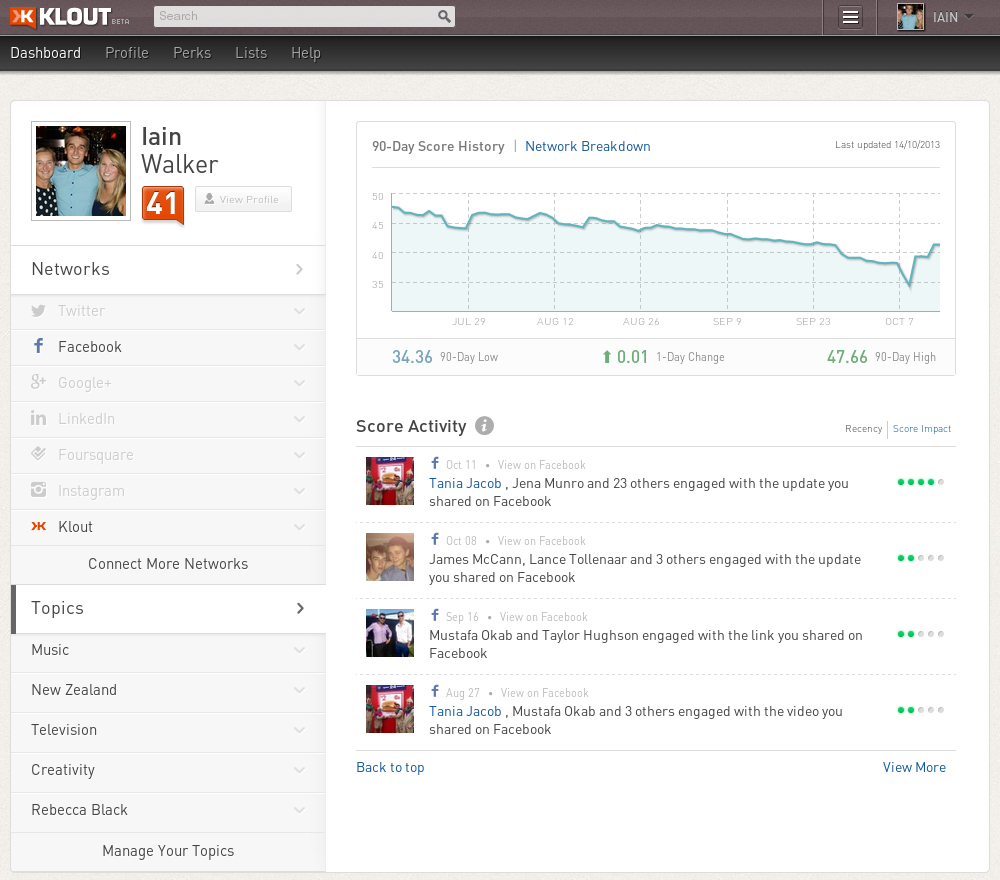
\includegraphics[width=0.7\textwidth]{Images/klout.png}
\caption{Klout impact score}
\end{figure}

\subsection{Discussion}

My proposed solution extends and borrows concepts from these related reputation systems. GRAft as a distributed reputation storage system has the potential for storage of reputation data for many different applications. By implementing reputation policies for storage within GRAft, I essentially create source nodes as a further case study example for this system. Whilst the Open Social based reputation system is useful for access control schemes, there was little discussion relating to other potential applications of its reputation schemes. As such it is of arguably less value than a more generic system such as GRAft. 

Whilst Klout provides interesting reputation insight into a users profile, it is limited in that only your own profile reputation data can be viewable immediately. To view friend's profiles, they must sign into Klout themselves. It is impossible to view the Klout scores for strangers. As such this system is only purposed for competition among friends, and little else. 

%Add more reflection and discussion about the related systems, and discuss why a new solution needs to be developed. Otherwise, why don't we just tsick with the current system lol

%Discuss how my system is different from these related systems, and how it adds value. 

%Graft system

%Klout

%How did my research relate to the existing works reviewed, and to what extent my work can be distinguished from them. 
\chapter{Methodology}\label{C:us}

\section{Project Management Approach}

The project was structured around a loose waterfall approach. At the start of the project, a long-term plan and major milestones were outlined. More detailed plans were added and target dates adjusted as the year progressed. Aspects of agile development practices were also used during the implementation and design stages. Throughout the project I had joint weekly meetings with Dr. Kris Bubendorfer,  Ferry Hendrikx and Filip Dimitrievski. In these meetings, 30-45 minutes in length, we were able to outline progress achieved during the week, any issues encountered,and solidify project direction. Having meetings with Filip and Ferry present was beneficial, as there were aspects of the project which Filip and I were able to collaborate over. Ferry, co-designer of the GRAft system was also able to give useful technical feedback, with his experience in the development of web-scraping tools.

This approach of combining aspects of waterfall and agile was reasonably effective as a project management approach. Agile methods tend to work best in a team environment, assisting with the coordination of team members. However the method of small, focused sprints contributing to the larger project were excellent in maintaining focus and direction. The waterfall element in turn outlined the more concrete and long-term goals of the project, which was useful with monitoring and controlling and ensuring my work did not fall behind.

These target goals were met in the majority of cases. I did experience delays with finishing my implementation and evaluation, as new goals such as community detection were added late in the project. Reasons for this late discovery and delay were in part due to the exploritory nature of the project, as discussed in the design approach. %CHANGE THIS TO SPECIFIC SECTION

%Design practices - strong prototyping approach. Only way to test if sites were feasible was through building prototypes. Benefit of learning how to web-scrape pages was also covered with this approach. 

%Weekly sprints, with stories to be completed by the end of each week during implementation. 

%Weekly meetings with Dr. Kris Bubendorfer and Filip Dimitrievski, as well as Ferry Hendrikx useful to get feedback. 

%Target goals - weekly goals were met the majority of the time, but focus of the project was in flux as priorities changed during implementation. 

%The project was structured around a loose waterfall approach. At the beginning of the project, a long term plan and major milestones were outlined

\section{Design Approach}

Requirements analysis and design were completed through a combination of research and prototyping. As the project was focused on an exploration of understanding reputation data on social media, a large portion of time was given to background research. This will be covered in depth in chapter 3.

Later in the design phase, I constructed a set of prototypes to evaluate the feasiblity and alternatives for a web-scraping solution. These covered preliminary scrapers for Twitter, Facebook, LinkedIn and Slashdot. The benefit of developing these was to both give me a better understanding of technologies involved with performing these functions, and to produce some meaningful effort early in the project, as these scrapers could be potentially useful later. There were some pitfalls in this approach however. It is noted that some effort in prototyping can go to waste - and this was the case here. We eventually declared web-scraping Facebook largely infeasible, due to its user interface's constant state of flux. Also during prototyping, Twitter's API changed significantly, rendering much effort lost. 

The weekly meetings with my supervisor allowed opportunities to obtain feedback on design choices, as well as suggestions where there was room for improvement. 

%Comes very close to being reflective, so would be worth just doing a reflective segment here!


%Need to discuss why such a loose project management and design style was appropriate for the project.

%Reference? Perhaps reference a prototyping design approach.
%Prototyping to achieve understanding. Weaknesses - some wasted effort. Facebook scrapers were eventually abandoned. Twitter API changed. etc etc
%Gantt Chart Here

\section{Project Complexities}

The complexity of the system stems largely from the aggregation of unstructured data from a variety of sources - a difficulty often encountered in web-crawling applications. The codebase itself is not overly complex. However, what contributed to the primary difficulty of prototype development was the development of code in the aggregation of data from disparate locations, and debugging often unclear and unexpected errors from various web requests. 

Understanding the data gathered was a time-expensive challenge. The process of understanding and defining reputation data on social media was the task that occupied most of my time on the project. 

The time constraint of 300 hours impacted the project at all stages. The implementation and evaluation components were particularly impacted - limitations had to be placed upon the scale of data collected from scrapers in order to compensate for time. In addition, the selected prototyping methodology was often expensive in terms of time, due to the necessity of revising code and collecting more relevant data, as I achived greater understanding of the problem domain. 


Understanding reputation data, and writing policies to describe reputation effectively.\\


Debugging and collection of data, and asserting that this data is avalid. Ensuring that websites were not overloaded, resulting usually in scrapers being blocked. Recovery from detection, and how scrapers can respond. Construction of useful policies, and data analysis and aggregation. 

%Aggregation of non-structured content from a variety of sources. 

%Debugging, collection of data. Avoiding detection by websites, and ensuring that websites were not overloaded, resulting usually in scrapers being blocked.
%Recovery from detection, and how scrapers can respond. Construction of useful policies, and data analysis and aggregation.


\chapter{Requirements Analysis}\label{C:us}

To satisfy the goals of the project, the following issues need to be addressed. The requirements may be logically split into two divisions; web-scraping requirements and access policy requirements.

\subsection{Functional Requirements}

\begin{description}
 \item [R1.] Policies must consider data from reasonable time periods, to generate a shadow of the future.
 \item [R2.] Aggregation of social media data into consistent and readable format
 \item [R3.] Metric of reliability based on amounts of data collected.
\end{description}

\subsection{Non-Functional Requirements}

\begin{description}
 \item [R4.] Resistance to User-Interface Change
 \item [R5.] Reasonable performance - expectation that policies and scrapers could be used as part of wider application.
 \item [R6.] Accuracy of data collected - content should not be missing or incorrect
 \item [R7.] Resistance to Blocking Detection - my scrapers should not be blocked.
 \item [R8.] Extensibility and Social Media Portability for future use of framework
\end{description}

\subsection{Discarded Requirements}

\begin{description}
 \item [R8] Aggregation of Social Media data, for storage in GRAft.
\end{description}


\section{Policy Construction}

The first and most significant requirement is to generate a set of policies to assist with generating a snapshot of the reputation information of an individual. 

\section{A reliability Metric Based on the Amount of Data Considered}%Consider removing this requirement

From the beginning of the project I acknowledged that it may not be feasible to scrape the profile or data of an entire user 

\section{Social Media Platform Portability}%Ability to port original scraper onto new sites.

The ability to build scrapers for new sites on top of existing architecture I develop.

%How to port my scrapers between social media platforms.

\section{Maintainability and Resistance to User-Interface Changes}

Along with portability of my scrapers, they need to be somewhat resistant to change at the user interface level. An oft-repeated downfall of web-scraping is that changes to interfaces may occur at any time, without warning. This is in contrast to changing APIs, which generally give some significant warning and phasing out period of functions. Often changes to the layout of pages will break crawlers, resulting in a need for frequent re-builgs on sites that go regular user interface change. As such my system must be designed in a manner that is as un-reliant on layout-specific information as possible. In cases where change will unavoidably break my scrapers, they should be designed in a fashion which allows for easy identification and solving of issues.

\section{Scraper Performance}

This requirement refers to the speed and accuracy of my web-scrapers. The web-scraping tools developed must perform with sufficient speed to generate snapshots of an individual's reputation, in a reasonable amount of time. In order to create policies that are useful for future works, these scrapers must be able to gather and make conclusions about an individual in a matter of seconds or minutes. Data gathered must be accurate and represent what is actually displayed on a site. 

\section{Ability to Resist Blocking Detection and Recover from Failure}

A challenge presented in web-scraping is the ability to resist detection as a robot by webservers. Webservers do not look well upon robots, and will attempt to block aggresive crawlers. As such my scrapers need to implement strategies to avoid detection, and when blocked or detected, take appropriate action. A balance has to be achieved between performance of scrapers and detection by webservers - normally a scraper attempting to retrieve masses of results will be detected and blocked extremely rapidly. 

\section{Privacy Protection}

This requirement refers to the fact that data I gather should be anonymised to a reasonable extent, such that actual personal details should not be traceable. 

Maintain reasonable privacy of data I collect. Discuss how the information I am gathering is publicly avaialble on social media anyway, and users should have reasonable expectation that their data will be accessed. 

\section{Discarded Requirements}

Aggregate data for storage into GRAft - because of community effort required. Business model would need to be constructed, out of scope for the project.

Visualisation component of the project-  discarded as was able to source external tools to visualise and represent data. 


%\subsection{Policy Requirements}

%\begin{number}
%\item Develop a set of Policies that can be used to ...
%\item Develop a metric of reliability of information gathered, based on privacy settings.
%\item Potential to Develop an Interface with Filip Dimitrievski's project. Re-using my web-scraping libraries could be useful for his project. (Probably not going to happen)
%\item Aggregate data for storage into GRAft
%\end{number}

%\subsection{Web Scraping Requirements}

%Web-Scraping Requirements
%\begin{number}
%\item Privacy Protection
%\item Maintainability and Resistance to User-Interface Changes
%\item Performance of Scrapers
%\item Ability to Resist Blocking Detection, and Recover from Failure
%\end{number}

\chapter{Scraper Design and Implementation}\label{C:us}

In this section I discuss the design and implementation of the web scraping components of the project. I highlight important decisions made during the course of the project, as well as steps taken to implement the system based on requirements detailed in chapter four.

%\section{A Prototyping Approach}

%Talk about how the design was constructed.

%My approach to prototyping and the problems this revealed.

%The overall design of my scrapers was largely developed through a prototyping approach early in the project. I performed research and web-scraping frameworks and technologies to decide which would best suit the requirements defined in chapter 4. The prototyping strategy also allowed me to investigate the feasiblity of scraping from different sites.

%By developing prototypes for Facebook and Twitter early in the project I was better able to 

\section{Architecture}

Two potential architectures were considered when designing the web-scraper components.

\begin{itemize}
 \item A database storage approach
 \item A text/XML storage approach
\end{itemize}

Having received feedback on the database approach, the more straightforward and suitable text/XML design was ultimately used.

\subsection{Database Storage Architecture}

\begin{figure}[h!]
 \centering
 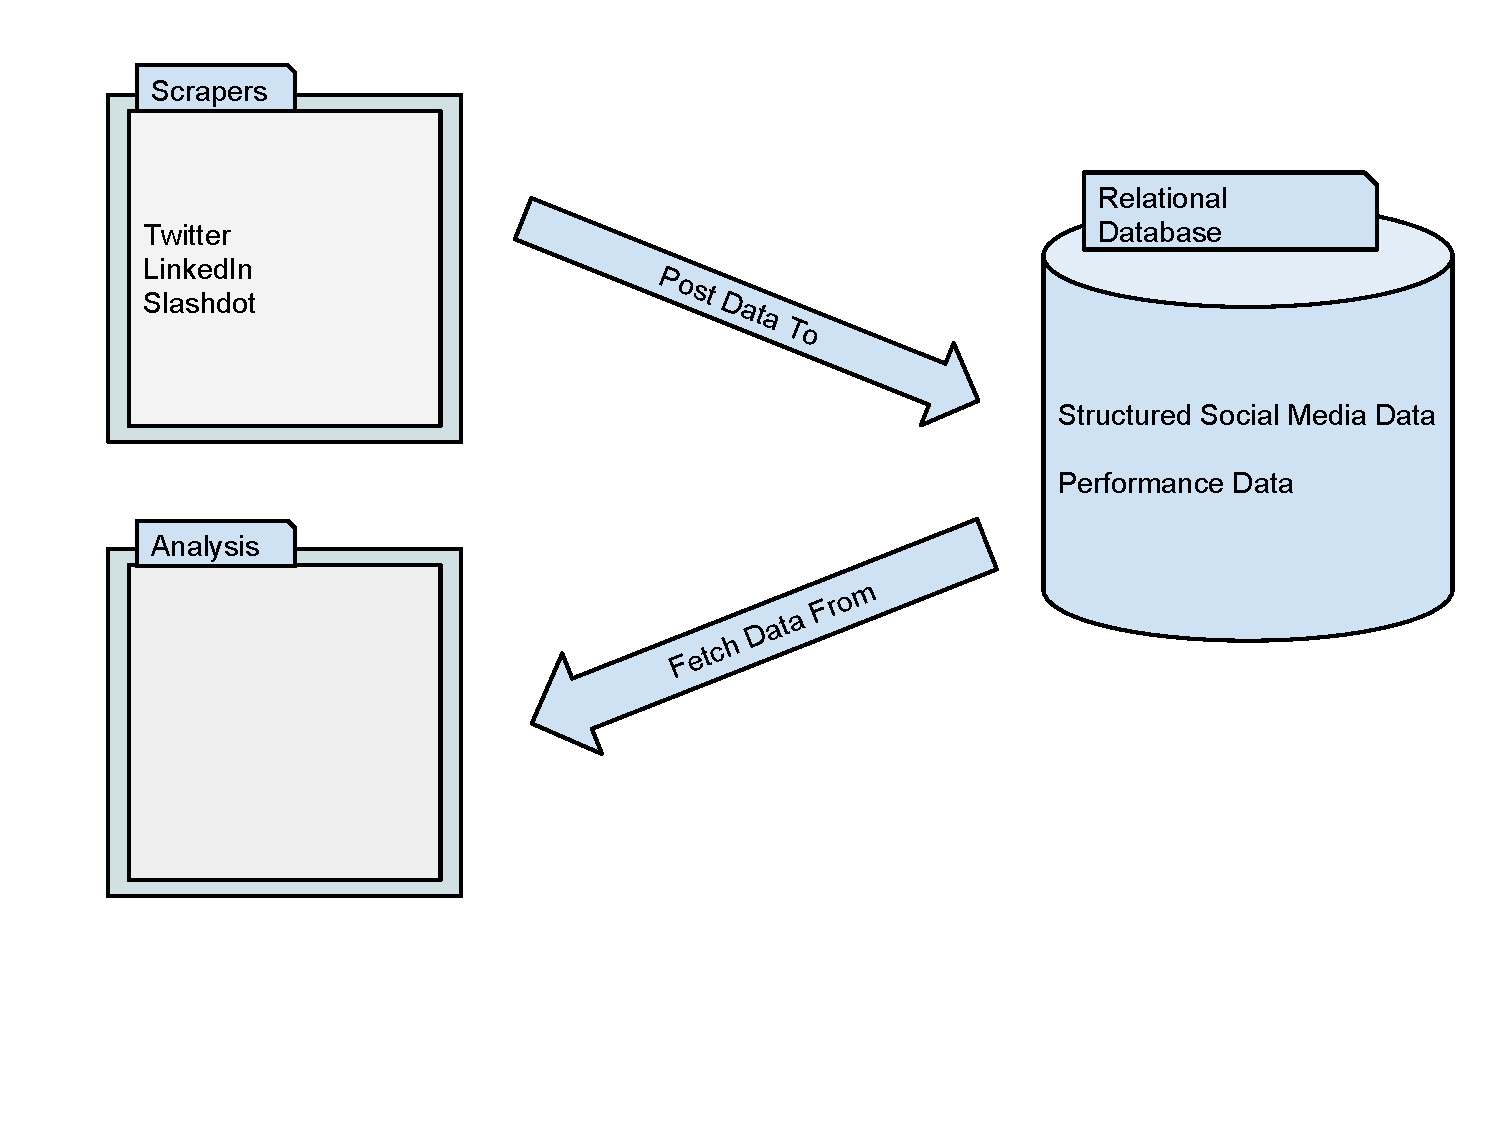
\includegraphics[width=0.7\textwidth]{Images/Database_Architecture.pdf}
 \caption{Proposed Architecture for Database Storage Solution}
\end{figure}

A possible approach to meeting the requirements of the project was to store fetched data in a relational database. In this design, the scrapers would gather data over an extended period of time, writing retrieved information into a database. Analysis components would then fetch data from the database as necessary, saving results in seperate tables within the same schema.

This approach provides long-term extensibility benefits, as per requirement R.4. All of the advantages that come with database storage would have been present in this solution - fetching of specific profiles for example would have been much more practical through a database query. 

However this design was deemed to be over-engineered for the purposes of the project. Given that data retrieved is in HTML, JSON or XML format there is a large impedance mismatch between retrieved data and relational database tuple format. This is compounded when retrieving data from the store for analysis - many third party analysis tools require input data in a variety of text forms.  The analysis components were also largely contingent on the fetching of a whole profile, rather than specific elements, lessening the need for querying against specific elements in my data storage structure. 

\subsection{XML Storage Architecture}

The alternative and ultimately selected architecture involves the scraper and analysis components interacting with a shared XML storage structure. Again in this structure, scrapers run over time whilst saving data to a common XML-based file system. Analysis components could then annotate and enrich the original dataset. 

\begin{figure}[h!]
\centering
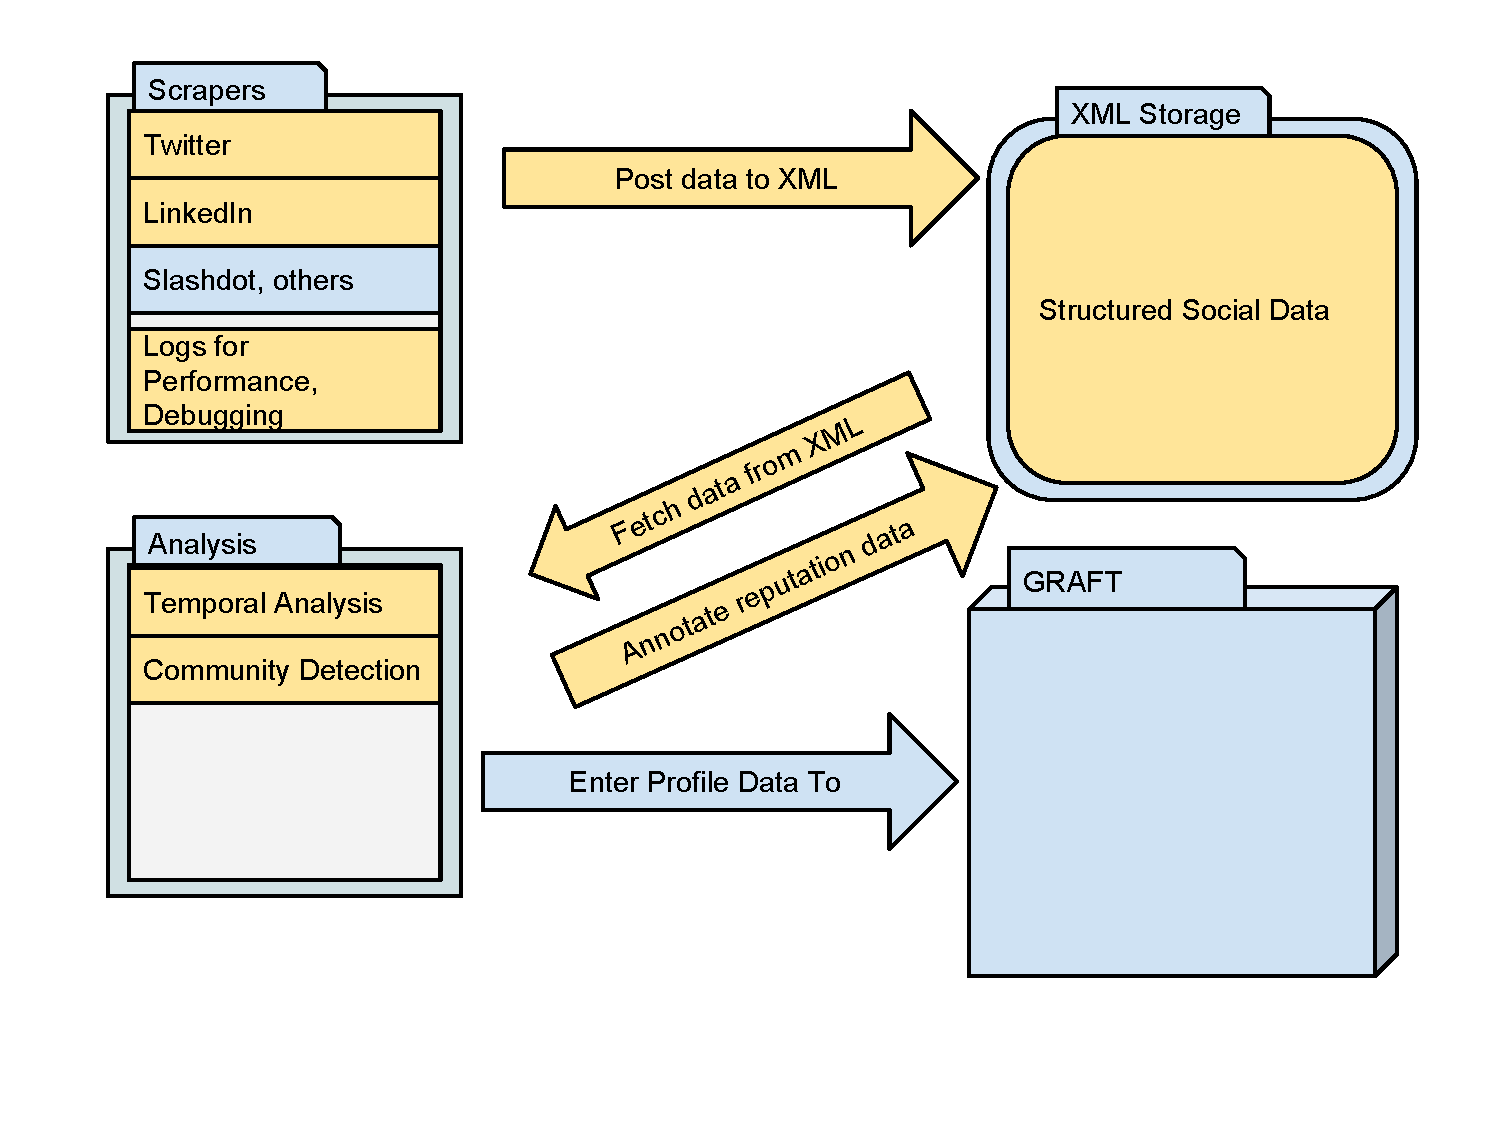
\includegraphics[width=0.7\textwidth]{Images/XML_Storage_Architecture.pdf}
\caption{Architecture for XML Storage Solution. Implemented Components are Highlighted Yellow}
\end{figure}
%File storage is also much faster and less server taxing than using a database
This design largely simplifys the scripting and scraper construction. Little setup was required during prototyping to construct schemas against which to save data. An informal XML approach also allowed for straightforward manipulation of data structures, and additions to what was being stored. Performance of storing to files is also known to be much faster and less server-taxing than the use of a database.

The primary disadvantage to the XML approach is difficulties associated with selecting individual slices of data in XML. Technologies such as xQuery exist for querying against XML, but were deemed unecessary for the project. This is due to entire profiles being used for input into analysis components, rather than selected components only.

\section{Technology}

The web-scraper components were written entirely in Ruby. The development of screen scrapers is largely independant upon language choice; however Ruby was selected due to its large number of libraries suitable for scraping, and straightforward scripting nature. Ruby also has a significant OpenSource following in comparison to many more conventional languages like Java. This was considered necessary early in the project, when looking at a model for future maintenance of the scrapers, especially for the discarded requirement of aggregating data for GRAft. 

Alternatives to Ruby were considered; Java, which does not have the same open source following as Ruby, as well as a larger degree of lower-level network coding for web-scraping software; and PHP, which was rejected due to time constraints limiting personal capabilities to learn the language to a competent level during the project. PHP would have given the advantage of being more consistent with past works, however \cite{GRAft}, as well as being the same language as my policies are described in. 

The frameworks upon which my scrapers were built included:

\begin{itemize}
 \item Nokogiri: a widely used HTML and XML parsing framework, allowing for straightforward interpretation of raw HTML documents.
 \item Mechanize: an extension of the Nokogiri framework, that simulates browser actions on web-pages.
 \item Rest-Client: Ruby's most popular HTTP client.
\end{itemize}

Alternative frameworks were considered, and their advantages and reasons for not being selected in the final model will now be covered.

\subsection{Extend scrAPI}

scrAPI is a Rubyforge project, allowing for fast implementation of web scrapers. The core benefit of scrAPI is allowing data to be fetched from HTML pages using CSS selectors. In addition it hides processes such as the actual fetching of pages. It is a much higher-level framework than Nokogiri and Mechanize. 

Extending scrAPI was ultimately discarded, due to its heavy reliance on CSS files remaining constant. Any change to stylesheet files would likely have broken the scrapers. Arguably these stylehseets are less likely to change than layout manipulations (for example consider xpath on HTML as an alternative); however on sites such as Twitter and Facebook large design teams frequently make changes to these files. Given that a key requirement of the project was to make scrapers resistant to user-interface change, this resulted in scrAPI being deemed unfit for purpose. 

\subsection{Extend A Browser-Automation Model}

Browser automation options were considered as an alternative architecture. Frameworks such as Watir allow users to simulate user interaction with web pages, by driving an actual browser instance.

A brower automated-scraper would likely have had little problem with site detection or blocking, due to the use of a real browser - providing genuine user agents, downloading css selectors and such. Despite this, performance would have been significantly poorer using this option. As browser automation scripts are generally highly dependant on site layout and interface naming conventions, this would have violated the requirement of resisting user interface change (R5). 

\subsection{Use the API}

Although the project title from the outset was 'Reputation Scraper', we investigated the use of site's APIs before settling on the scraping option. A basic application interacting with the Twitter API was constructed early in the project. Twitter's API version 1.0 was actually highly suitable for the needs of the project. However the changes in REST API v 1.1 rendered this infeasible. The earlier API allowed fetching of up to 800 statuses from any public profile, along with more public data (see appendix for more information). Version 1.1 however implemented more requirements for authentication, and limited functions such as downloading tweets to the individual's account only. Facebook's developer API is even more restricted. On Facebook, permissions must be obtained from the appropriate users before fetching data from their profile. LinkedIn's policy is similar. %due to the changes!!!

\begin{figure}[h!]
\centering
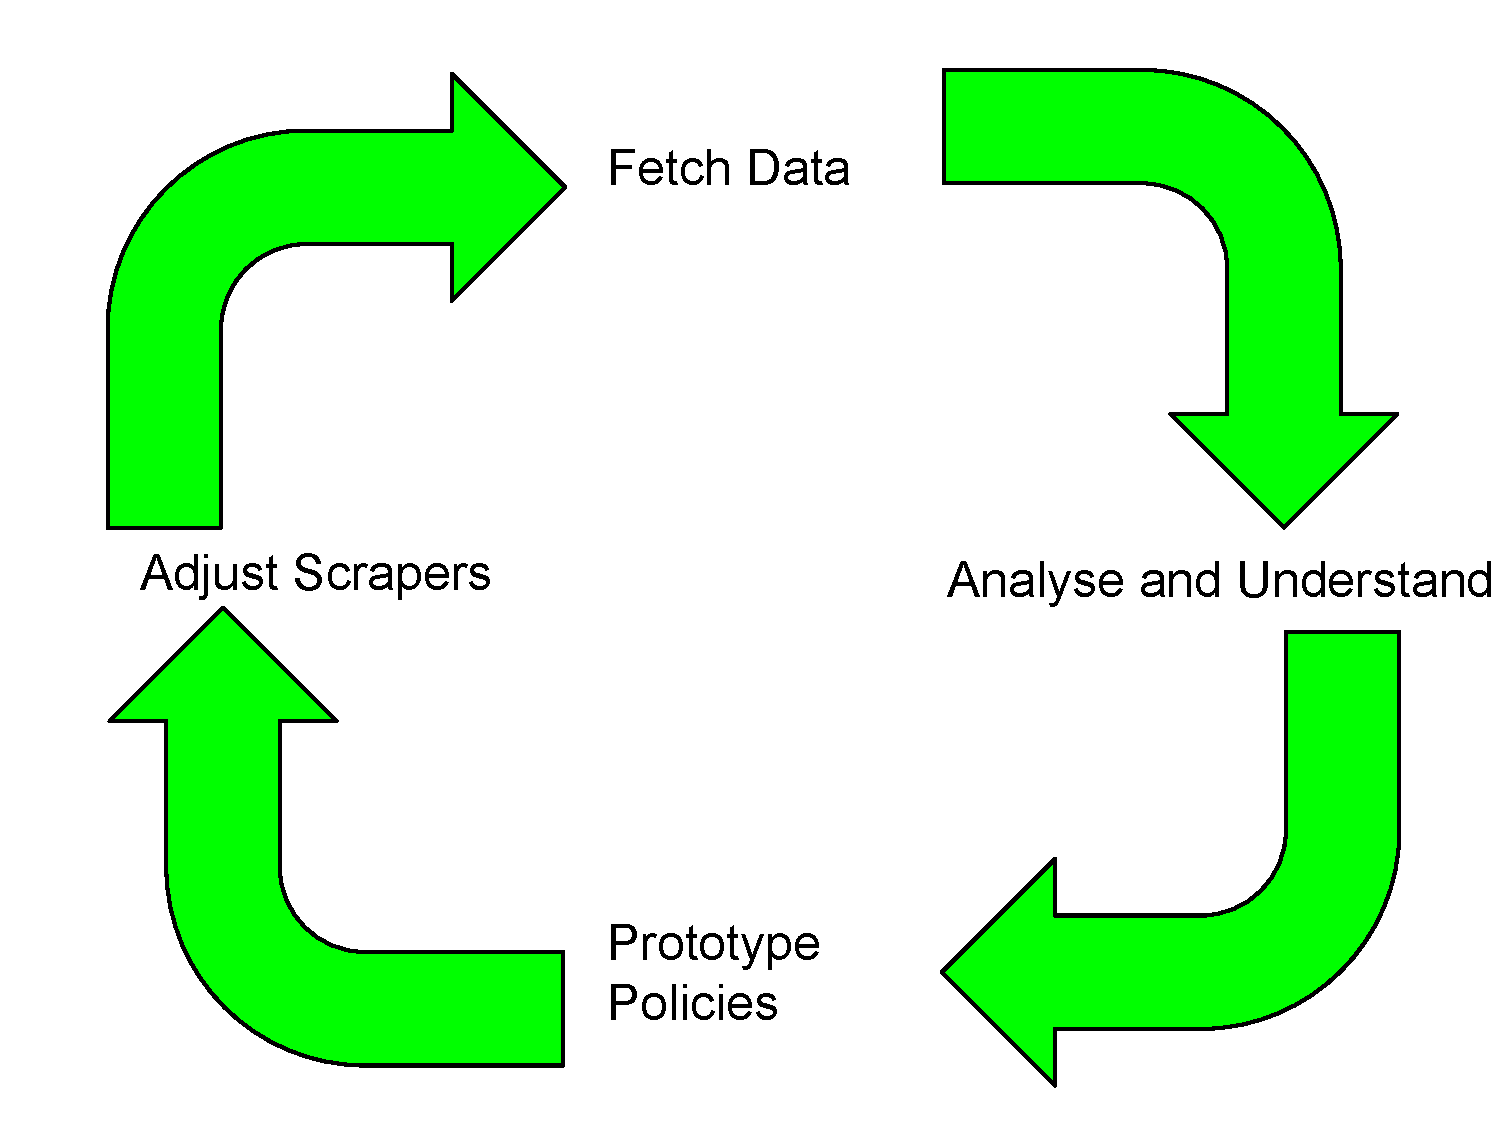
\includegraphics[width=0.4\textwidth]{Images/Implementation_Lifecycle.pdf}
\caption{Scraper Development Feedback Loop}
\end{figure}

\section{Systems Design and Structure}

Developing the project solution consisted generally of a cyclic, iterative prototyping approach as detailed in figure 5.3. This generally consisted of four phases; Implementing and adjusting scrapers, fetching data, analysing the data, and prototyping policy concepts as a result of this analysis. The first scraper developed was for Facebook. 

\begin{figure}[h!]
\centering
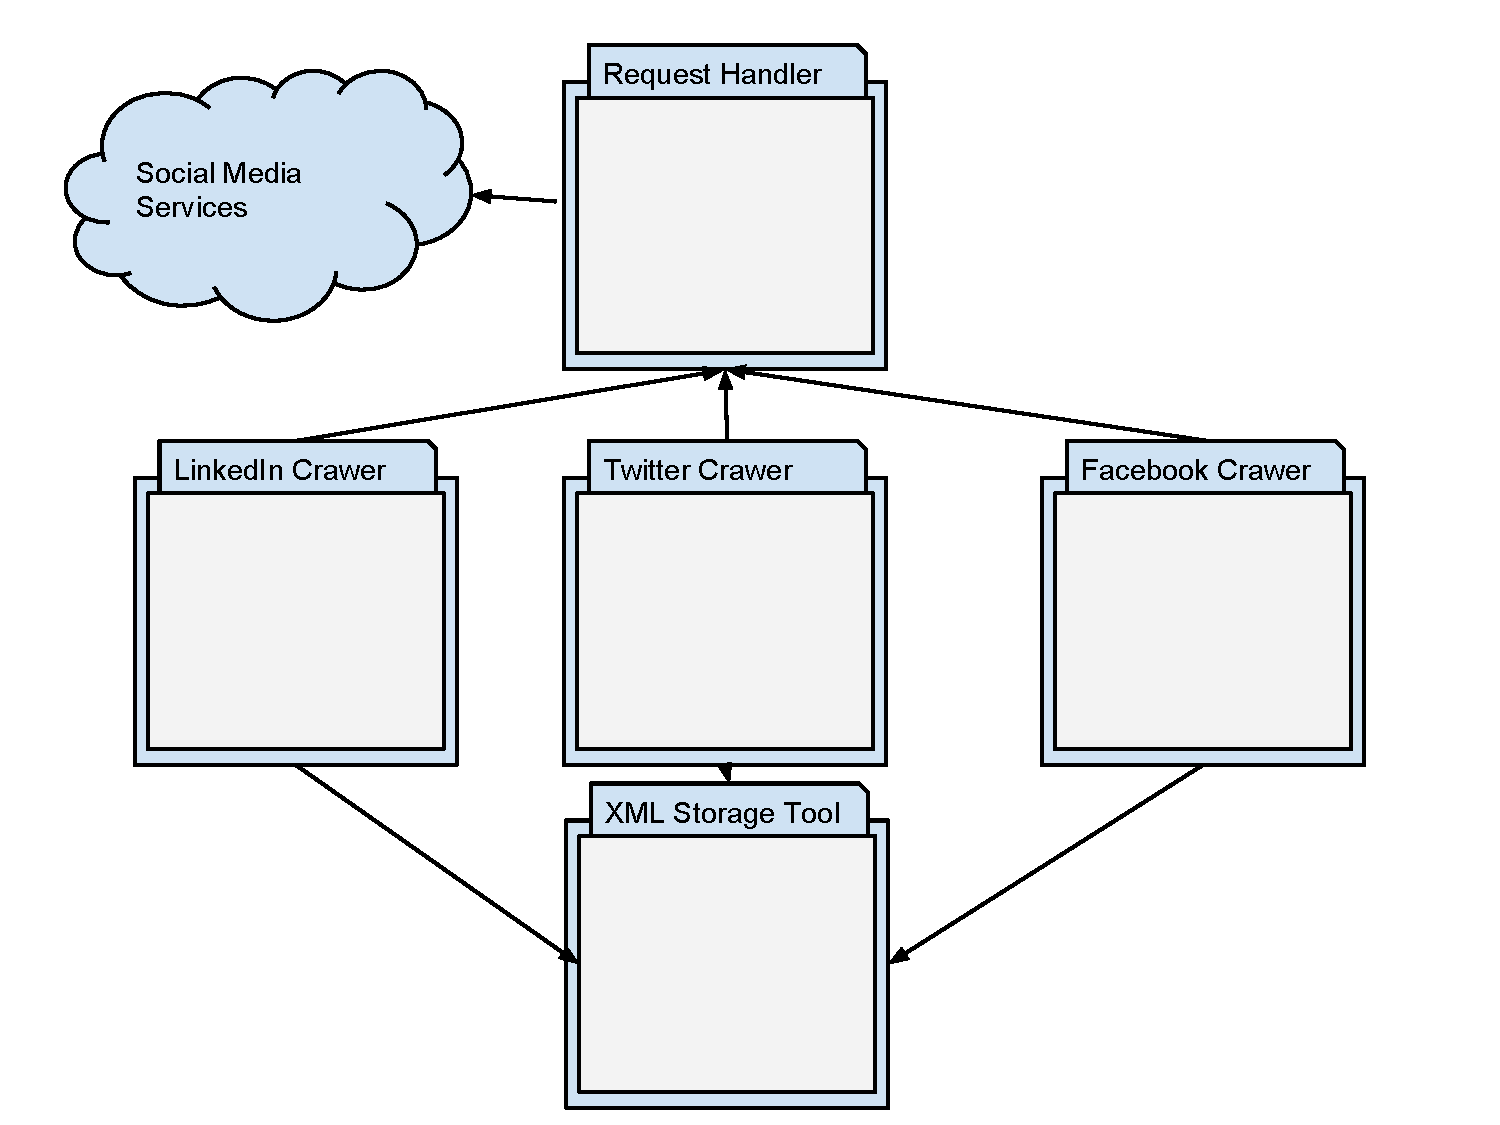
\includegraphics[width=0.6\textwidth]{Images/Code_Reuse.pdf}
\caption{Pipes-and-Filters Class Structure}
\end{figure}

\section{Facebook Crawler}

A Facebook scraper was prototyped early in the project, and allowed for experimentation with many of the technologies that were used later. Firstly, strategies for authenticating against Facebook had to be developed. While public profiles do exist, these are primarily for company pages or politicians, which is not what the project aimed to soley investigate. Authentication was implemented using a dummy Facebook account, through the Mechanize Ruby framework. Mechanize allows for form data on pages to be populated and submitted through either HTTP or HTTPS. Once authentication was achieved, an auth token was passed as an attribute of futher requests. New auth tokens are obtained after an adjustable time period, or on a new scraper run. 

Having obtained the necessary authentication tokens, profile pages could be fetched. The planned approach was to crawl through friend networks via friend lists, and scrape profiles in this manner. Downloaded profiles would then be parsed using Nokogiri, and relevant data extracted via xpath expressions. Posts, likes, friends are examples of information identified as useful to collect. However as mentioned in chapter 3, this scraper was eventually discarded as infeasible. Scraping large amounts of content reliably through Facebook was infeasible within the project's scope due to its highly dynamic content, and frequently changing interface. Maintaining and updating a scraper to fetch accurate data from Facebook during the project would have been too time-consuming and distracting, and as a result was removed from the project scope. However the technologies experimented with whilst developing this prototype were useful later when developing the more robust Twitter scraper.

%Discuss what I built the Facebook prototype with. Then mention that the technologies used here were added to in order to make the Twitter Crawler. Discussion as to why this was discarded as a requirement.

\section{Twitter Crawler}

The Twitter Crawler users a Google Twitter search function to search for profiles to fetch at the top level. An input text file of random names delimited by lines is accepted by the scraper. These names are looped through in order, with the scraper fetching the profiles of these top ten results returned through Google. Bias is introduced through this approach, since only the top ten search results are analysed. 

%The Twitter Crawler uses a Google Twitter search function, to loop through profiles at the top level. An input text file of random names delimited by lines is accepted by the scraper. These names are looped through in order, with the scraper fetching the profiles of the top 10 results returned through Google. Bias is introduced through this approach, as results appearing in Google are naturally more popular than users who would not. However as the top ten results are fetched and prepared for scraping, in general the lower ranking users here are more 'standard'. 

Due to this bias, alternative approaches were considered. A potentially better scientific approach to randomising the selection of profiles to scrape would have been to crawl through an already-generated set of random profile names. However searches did not reveal any such databases to exist, excluding 'celebrity-exclusive' ones which would have been significantly worse than my current approach. I also considered crawling via embedded links on Twitter, starting from any profile and following retweet links through to new profiles. However this introduces new complexities - how will the algorithm detect infinite loops (potentially huge loops), or detect repeat profiles? As the project was ultimately about reputation and not scraping algorithms, the simple name-searching approach was selected. 

Once the ten profile names are selected (for the current input name in the text file), the application will perform the scraping of each of these profiles in order.  The definition of a Twitter profile changed throughout the project, as more information was chosen to be analysed. The final schema of stored data for the standard Twitter scraper is contained in appendix 1.1. Essentially all tweets are captured where possible, along with associated retweets, favourites, and the profile names of users who retweeted this item. Profile metadata is also stored, such as number of followers, number following, and total number of tweets. 
%CHANGE THIS AS APPROPRIATE. 

Technical difficulties exist with fetching such profiles and metadata, which we will now discuss. Firstly, a Twitter page does not immediately display all tweets for a user for obvious latency reasons. To view more than the initial tweets, users must scroll through an 'infinite scrolling' window which requests more data through AJAX calls. To simulate this interaction, I used Google Chrome's 'network capture' feature to inspect requests to the page during the scrolling function. The URL is of the following form:

\begin{verbatim}
 /timeline/with_replies?include_available_features=1&include_entities=1&max_id=12345
\end{verbatim}

\noindent The JSON returned is then parsed to retrieve relevant information. As a Twitter profile may contain retweets from other profiles, checks have to also be taken at this stage to ensure the content is originally generated by the user of interest. This is as simple as checking the user name who posted the content originally. In order to increase the performance of extra tweet fetching, various tweet window sizes were experimented with. This was ultimately inneffective at maximising speeds, reasons for which are covered now.

\subsection{Parallel Tweet Fetching}

Although tweet content can be fetched from the base profile page, useful data such as retweet and favourite count is initially hidden. To view tweet detail, a further request must be sent, to mimick the user interaction of clicking on the tweet. Fortunately this process can be parallelised for each tweet within a tweet window. In the final twitter scraper a thread pool of 15 threads is created, one for each potential tweet in the window. Each thread then fetches and parses each tweet individually. To ensure parallel performance is not lost, any tweet-fetching process that fails here will simply be thrown away. Parallelisation of tweet fetching resulted in huge performance gains, which will be discussed further in chapter 6. Parallel fetching was not considered earlier in the project as I expected the resulting simulataneous requests to end in more frequent detection by sites. 

\subsection{Detection Avoidance and Recovery}

Operating on the University network likely resulted in less chance for blocking detection by Twitter, due to the large IP range allocated to Victoria University. Regardless, steps were taken to limit detection rates. Multiple strategies for avoiding detection were considered, and several employed simultaneously. The Request-Handler package handles the implementation of these strategies.

The first and most straightforward strategy is to include random pause times between requests. The goal of this approach is to reduce potential server burden, and lessen the possibility of an aggresive scraper being permanently blocked due to its flooding the site. However this approach imposes a very low ceiling for performance and tweet fetch rates. Resources such as \cite{} recommend a ten to fifteen second delay between requests, but such a wait was infeasible for the needs of the project. As such, pauses between requests were only implemented in certain special cases; failed requests and at the end of a profile. 

The second strategy employed is to send requests that spoof a browser user-agent, in order to appear as a legitimate browser instance at the server end. Before scraping a new tweet window, a new user-agent string is randomly selected from a list. 

A third strategy that was considered but not implemented was the downloading of CSS and other markup, in order to behave as browser-like as possible. This was discarded because of questions of its feasiblity, as well as uncertainty as to the level of potential benefits from constructing such a solution. 

%Rate limiting detection
I rarely encountered rate limiting at University, and was never blocked outright on the University machines. Early in the project, when prototyping a Facebook scraper I was briefly banned from Facebook at home. 503 errors reveal detection on Twitter. 500 errors were encountered throughout the project also, but these were due to coding errors. 

\subsection{Dealing with Authentication}

The original scraper did not require authentication, since the majority of Twitter profiles are viewable to individuals who do not have a Twitter account, or are not signed in. However to fetch the names and profiles of users retweeting posted content, an authentication feature had to be added. Fortunately the authentication strategy employed by the Facebook prototype was able to be re-used for this component. 

To fetch retweet-name data, more features had to be added. All other data fetched was publicly viewable, whereas this data is only available to users who have authenticated with Twitter.

\subsection{Dealing with Poorly Formed Markup}

A concern earlier in the project was the scraping of content containing poorly formed HTML or JSON markup. Thankfully the sensitivity of HTML parsers to poor markup is largely library-dependant. This was not well-documented in the gems (a gem is the library equivalent in Ruby) I found, so experimentation with various options had to suffice. 

%Mention that the code is available from github. http://www.github.com/irwalker/dat-roll

%Content behind login

%Infinite scrolling

%Rate limiting -> encountered sometimes? 503 errors primarily

%'Scraper window', not actually very effective, due to the primary networking burden being on sending a seperate HTTP request to download every tweet.

%Spoofing headers -> using fake user-agents, and rotating between user agents in between overall requests.

%Poorly formed markup -> was an occasional issue. Found that some libraries were more strict on this than others, and adjusted accordingly.

%Authentication

%Pattern scraper employed to fetch data. 

\section{LinkedIn Scraper}

The LinkedIn Scraper was developed towards the close of the project, and as a result data analysis of what was collected using this tool was not carried out. %Discuss how the implementation of this component was a sucess in that it proved the extensibility of the framework developed. 

%brief description of the work done developing the LinkedIn scraper. What was fetched, etc etc.

\section{Code instrumentation}

The code was instrumented using a Ruby logger system written for the application. Given complexities and difficulties debugging errors on web-scraping applications, logging had to be performed to a very fine level of granularity. Any action changing system state such as fetching a page triggers the logging mechanism. The logger would then take note of the timestamp and write to the appropriate file the nature of the action. For example, if the scraper sent an HTTP request to retrieve a given URL, it would record the timestamp and URL requested. 

The logger would write to the appropriate log file based on the nature of the supplied action. Because these scrapers were running over long periods of time, using traditional IDE debugging tools was not effective at detecting errors. As a result, I used multiple debugging files with different purposes in an attempt to catch these errors. The debug.log captured all interaction information at a basic level. Error.log captures error information that is non-fatal to scraping an individual's profile, e.g. on Twitter. Commonly these errors were due to application logic flaws, such as performing operations on null entities. As a result the error.log assisted greatly in identifying these edge cases. Finally the failure.log was used to record fatal exceptions that would prevent me from scraping a profile. Occurences such as 404, 500 or 503 responses from servers are examples that would result in a record being written to the failure log. The failure log would write system state at the time of failure to a high level 
of detail, sometimes even writing the entire HTML document before the failure to disk. This again assisted with debugging, when reviewing how a particular run had gone. 

To limit the performance overhead of writing to these logging files, a buffered approach was taken in order to achieve the least impact. %lol

\chapter{Evaluation}\label{C:us}

This section outlines my evaluation strategies, tests performed, and presents and discusses the results of evaluation conducted on the developed web scrapers. It then presents an evaluation of the policies and hypotheses formulated during analysis of data gathered. 

\section{Scraper Accuracy}

http://www.beevolve.com/twitter-statistics/

\section{Performance Evaluation}

Given the iterative approach taken to develop the scrapers, I evaluate their performance with respect to incremental builds, as well as final performance. As the definition of a 'profile' differs between sites, different performance metrics are used for each site. 

Performance testing of scrapers was carried out throughout the project, through performance logging mechanisms designed to measure the time taken to fetch an entire profile. To reduce bias caused by varying network speeds at University, the software was run over extended periods of time.

\subsection{Twitter Performance Evaluation}

Twitter profiles consist of differing numbers of tweets, retweets and so on. Thus I evaluate the performance of my Twitter scraper with respect to average time taken to fetch and parse a tweet. The major limiting factor for scraping useful information from Twitter was that each tweet had to be fetched with a seperate HTTP request. 

Should mention that some profiles viewed (not necessarily scraped) can contain hundreds of thousands of tweets.

%What should I compare this to? 

\section{Web Scraper Evaluation}

Performance - what performance goals did I have. How did they improve over time. Justify use of the incremental prototype-based strategy, through performance gains throughout the project.

Resistance to Detection - what performance goals did I have.

Problems

Accuracy - issues and why. Aims that I had - don't think I achieved them. In general entire profiles were not scraped. 

\section{Scraper}

\subsection{Functional Requirements}

Aggregate data for storage into Graft - given that I am currently only storing data from Twitter this requirement has not yet been met.

Develop a metric of reliability of information gathered, based on privacy settings. Currently on Twitter there are two degrees of privacy - Open and Closed! Closed profiles means I cannot get any meaningful information, whereas on Open profiles I can get anything I want! Most profiles are open so this is not a concern. Profiles of celebrities etc are always set to open.

Developing a set of Policies - still in the production line, still experimenting with different ways of using the data.

\subsection{Non-Functional Requirements}

\subsubsection{Maintainability and Resistance of Scrapers to User Interface Change}
This is difficult to evaluate. Experiment: Change the layout of twitter pages, see how the scrapers react to these changes. How many changes do I need to make? There will undoubtedlu be single points of faiure, which I should mention. Important point: used as little xpath expressions as possible, as these inherently result in less flexbile scrapers. Any structural changes, or even a tag changing result in an xpath expression having to change. Still resistant to stylesheet changes, though.
Single points of failure.

I identify areas which will result in the scraper breaking. 

\subsubsection{Twitter Scraper Performance}
I evaluate the performance of my twitter scraper with respect to average time taken to fetch and parse a tweet. The major limiting factor for scraping twitter was that each tweet had to be fetched with a seperate http request. Figure <x> shows the average time taken to fetch and parse each tweet, with respect to my incremental build stages. The success of continuous and incremental improvement in performance helps justify my decision to use an incremental approach. Tweets were gathered over several days, and continuously throughout different times of the day on the Victoria network to ensure that a representative range of times were gathered for each stage. 


I evaluate the performance of my twitter scraper with respect to average time taken to fetch and parse a tweet. The major limiting factor for scraping twitter was that each tweet had to be scraped with a seperate http request. Figure <x> shows the average time taken to fetch and parse each tweet, with respect to incremental builds. This also helps justify my incremental development strategy - we can see that succesive builds gradually increase performance. Tweets were gathered over several days, and at different times of the day on the Victoria network to ensure that a representative range of network performance speeds were used to gather data.\\

\noindent The significant feature of improved performance was through parellization of tweet-fetches. 

\begin{figure}[h!]
\centering
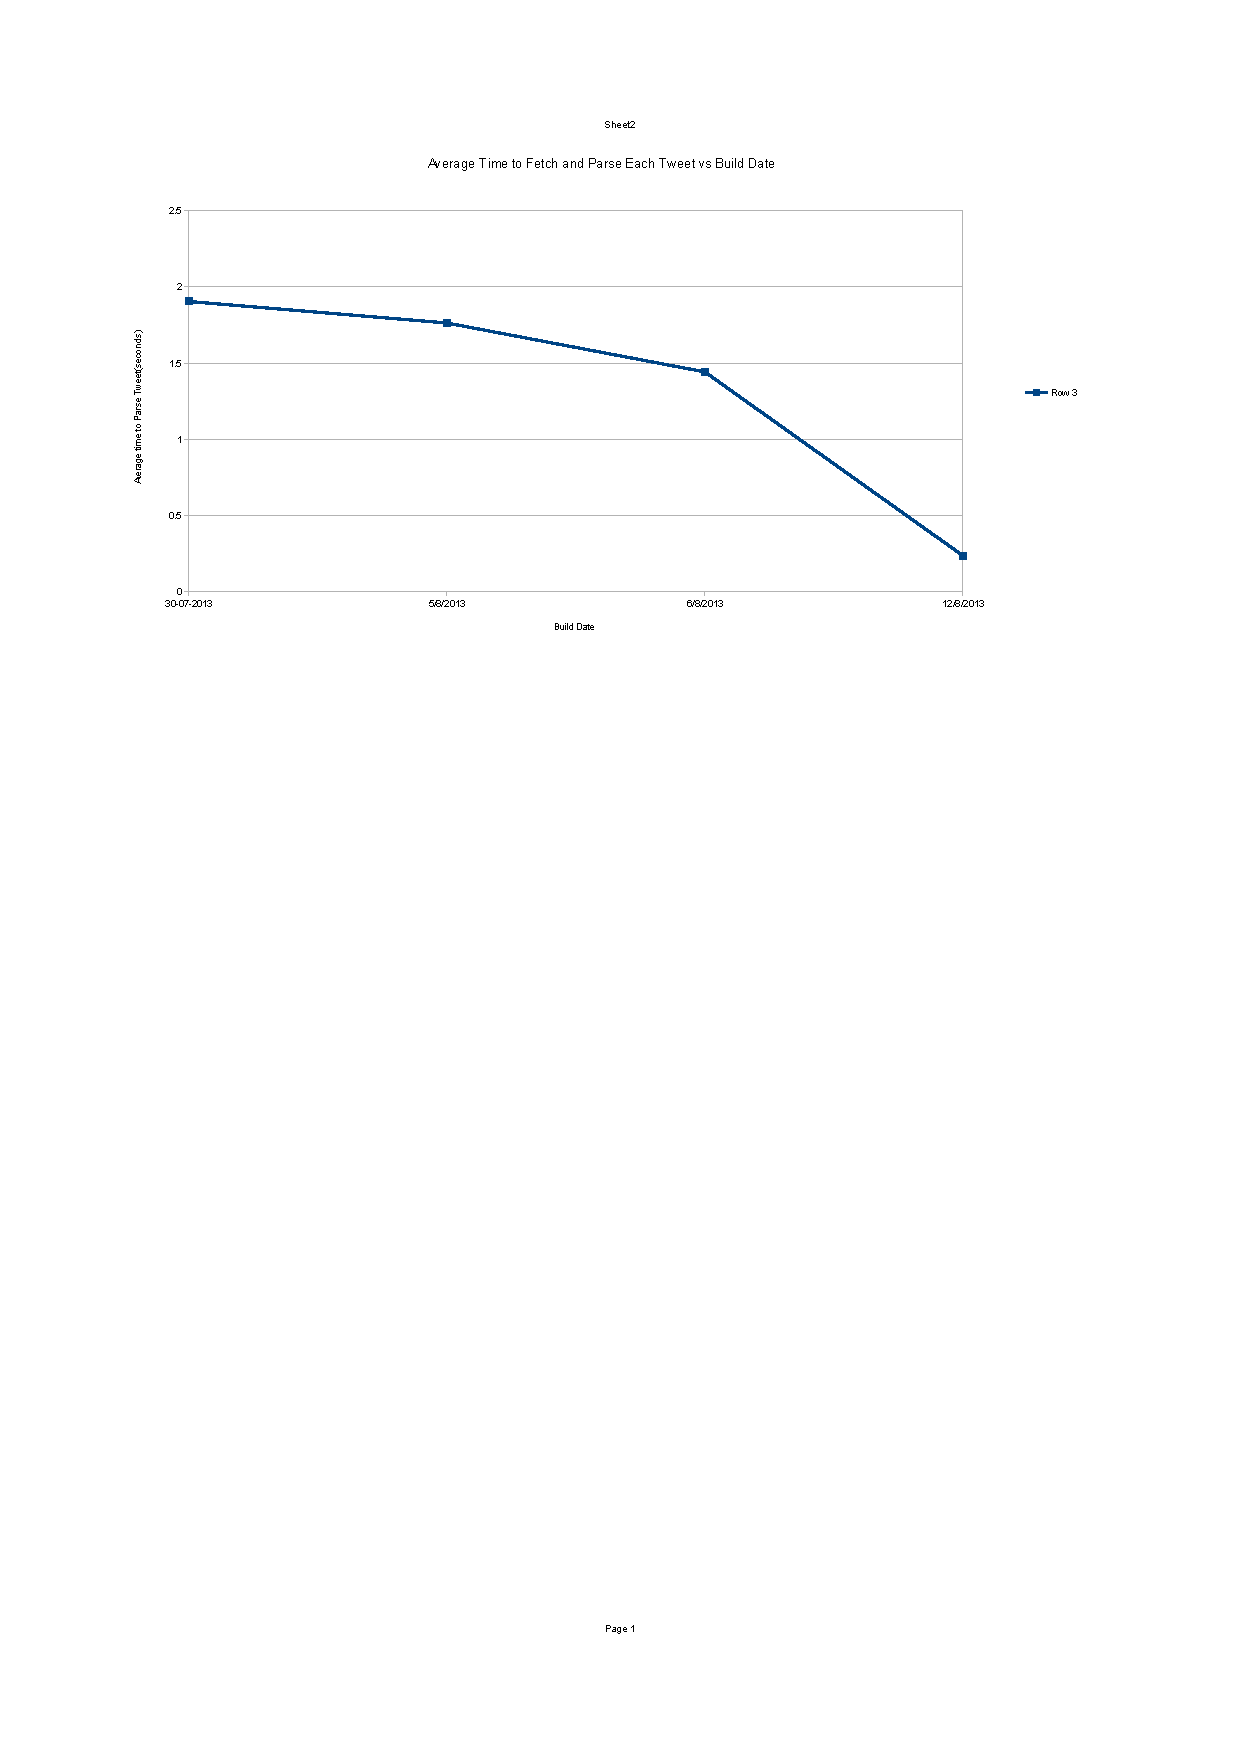
\includegraphics{Images/average_time_to_fetch_parse_tweets_per_build.pdf}
\caption{The Average Time to Fetch and Parse a Tweet, Ordered by Builds}
\end{figure}

Absolute limitations - Every tweet has to be fetched in an individual http request. This produces upper limits as to how fast the scraper can go, and means that the majority of performance speed is reliant on the speed of the network. (data - show how on some days tweets are fetched slightly faster than on other days. Times of day.)

\subsubsection{Ability to Resist Blocking Detection}

The primary measure of my scraper libraries avoiding blocking detection is with regards to their failure or incomplete-scrape rates. Although in early, less stable builds I had parsing errors, my later work only failed when detected by twitter and blocked. As such detection rates in later builds can reliably be calculated by analysing failing or incomplete twitter profiles. 

\begin{figure}[h!]
\centering
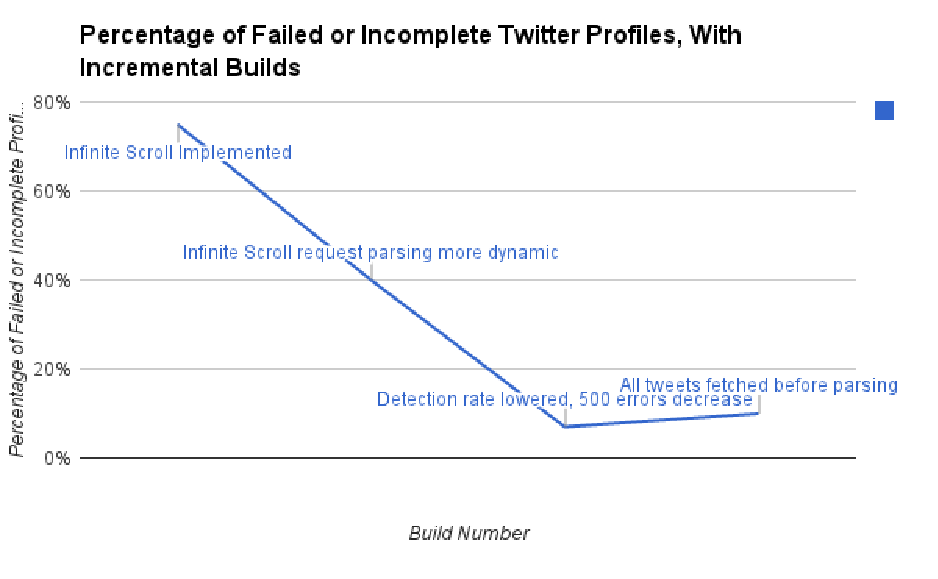
\includegraphics{Images/percentage_failed_incomplete_twitter_profiles.pdf}
\caption{The Percentage of Incomplete or Failed Profile Scrapes, Ordered by Builds}
\end{figure}

\subsubsection{Privacy Protection}

Privacy protection - this is still pretty poor, saved as structured xml, data not anonymised (makes my life easier at present)... Are there things I could be doing here potentially to increase privacy for individuals that I am scraping? Document locking, or store as RDB? Since I plan on storing this info in Graft, this could be anonymised at this point. Individual profiles and what-not. 

\section{Possible Improvements}

Greater parallelizaion - over the ECS Grid for example, rather than froma  single machine. Parallelize components other than tweet fething - entire profile fetching could be split up. Over engineered? 

\section{Scraping Conclusions}

Conclusions about what pages are suitable to scrape
\chapter{Data Discussion and Policy Construction}\label{C:us}

This section addresses the construction of reputation policies for use on Twitter. In particular the development of analysis tools for achieving greater understanding of the Twitter dataset created are discussed, and discussion of hypotheses generated from this data and how we experimented with these. Only Twitter data is discussed due to the richness of the dataset mined. As such multiple analysis approaches were taken.

Data was collected during scraper implementation, as per the feedback loop in figure 5.3. Profiles scraped earlier contain less detail than data collected later. For example, names of retweeters was not a feature collected on earlier profiles. In total, 1767 separate profiles were scraped, totalling 1,745,161 tweets. 

%Twitter data is discussed soley, as the dataset retrieved was rich enough to provide for several analysis angles.
%Fix this

%\section{Collection Method}

%Data discussed was collected entirely from the Twitter Scraper I implemented. This was collected during implementation, as per the feedback loop in figure 5.3. As such, profiles scraped earlier contain less detail than data collected later. 

%Show the median,q1 q3 min max of the number of tweets per profile perhaps?

\section{Retweet Analysis}

Retweets were considered as a basis for policies as more semantic information can be retrieved from retweets than favourites. When retweeting content users are able to comment and add extra value to the post, whereas this is not possible for favourites.

The first question asked was to do with the use of retweet and favourite functionality on Twitter. When \textit{retweeting} content on Twitter, the post will appear on the users own wall, as a tweet. A \textit{favourite} instead is added to a user's list of favourite tweets, which may be viewed separately by other members of Twitter. To demonstrate policy examples later, and to simplify data collection, we put forward that tweets similar in popularity will have equivalent amounts of retweets and favourites. We hypothesise that as a measure of impact, the number of retweets and favourites for an item on Twitter are equivalent.

% \begin{description}
%  \item [H1.]{As a measure of impact, the number of retweets and favourites for an item on Twitter are equivalent.}
% \end{description}

A simple approach to demonstrate that the use of retweets and favourites is equivalent in terms of impact or response is to check the correlation between these figures on a set of tweets. Figure \ref{fig:correlation_retweet_fav} shows this correlation. We find that retweets and favourites have a strong positive correlation, with a Pearson's coefficient r of 0.875 (3.s.f), n = 1,048,576. 

\begin{figure}[h!]
\begin{center}
 \centering
\includegraphics[width=500px]{Images/retweets_vs_favourites.pdf}
\caption{Correlation of Retweet and Favourite Count}
\label{fig:correlation_retweet_fav}
\end{center}
\end{figure}

%Number of tweets compared against
%Correlation

\subsection{Impact Factor}

We created an /textit{impact factor} measurement based upon a Twitter user's retweet count, and tweet activity. This formula is upon the Hirsch-index \cite{hirsch2005index} measurement for an academic's contribution to literature. It attempts to measure both the impact (number of retweets) and productivity (number of tweets) of a Twitter user. 

\begin{figure}[h!]
\begin{center}
\centering
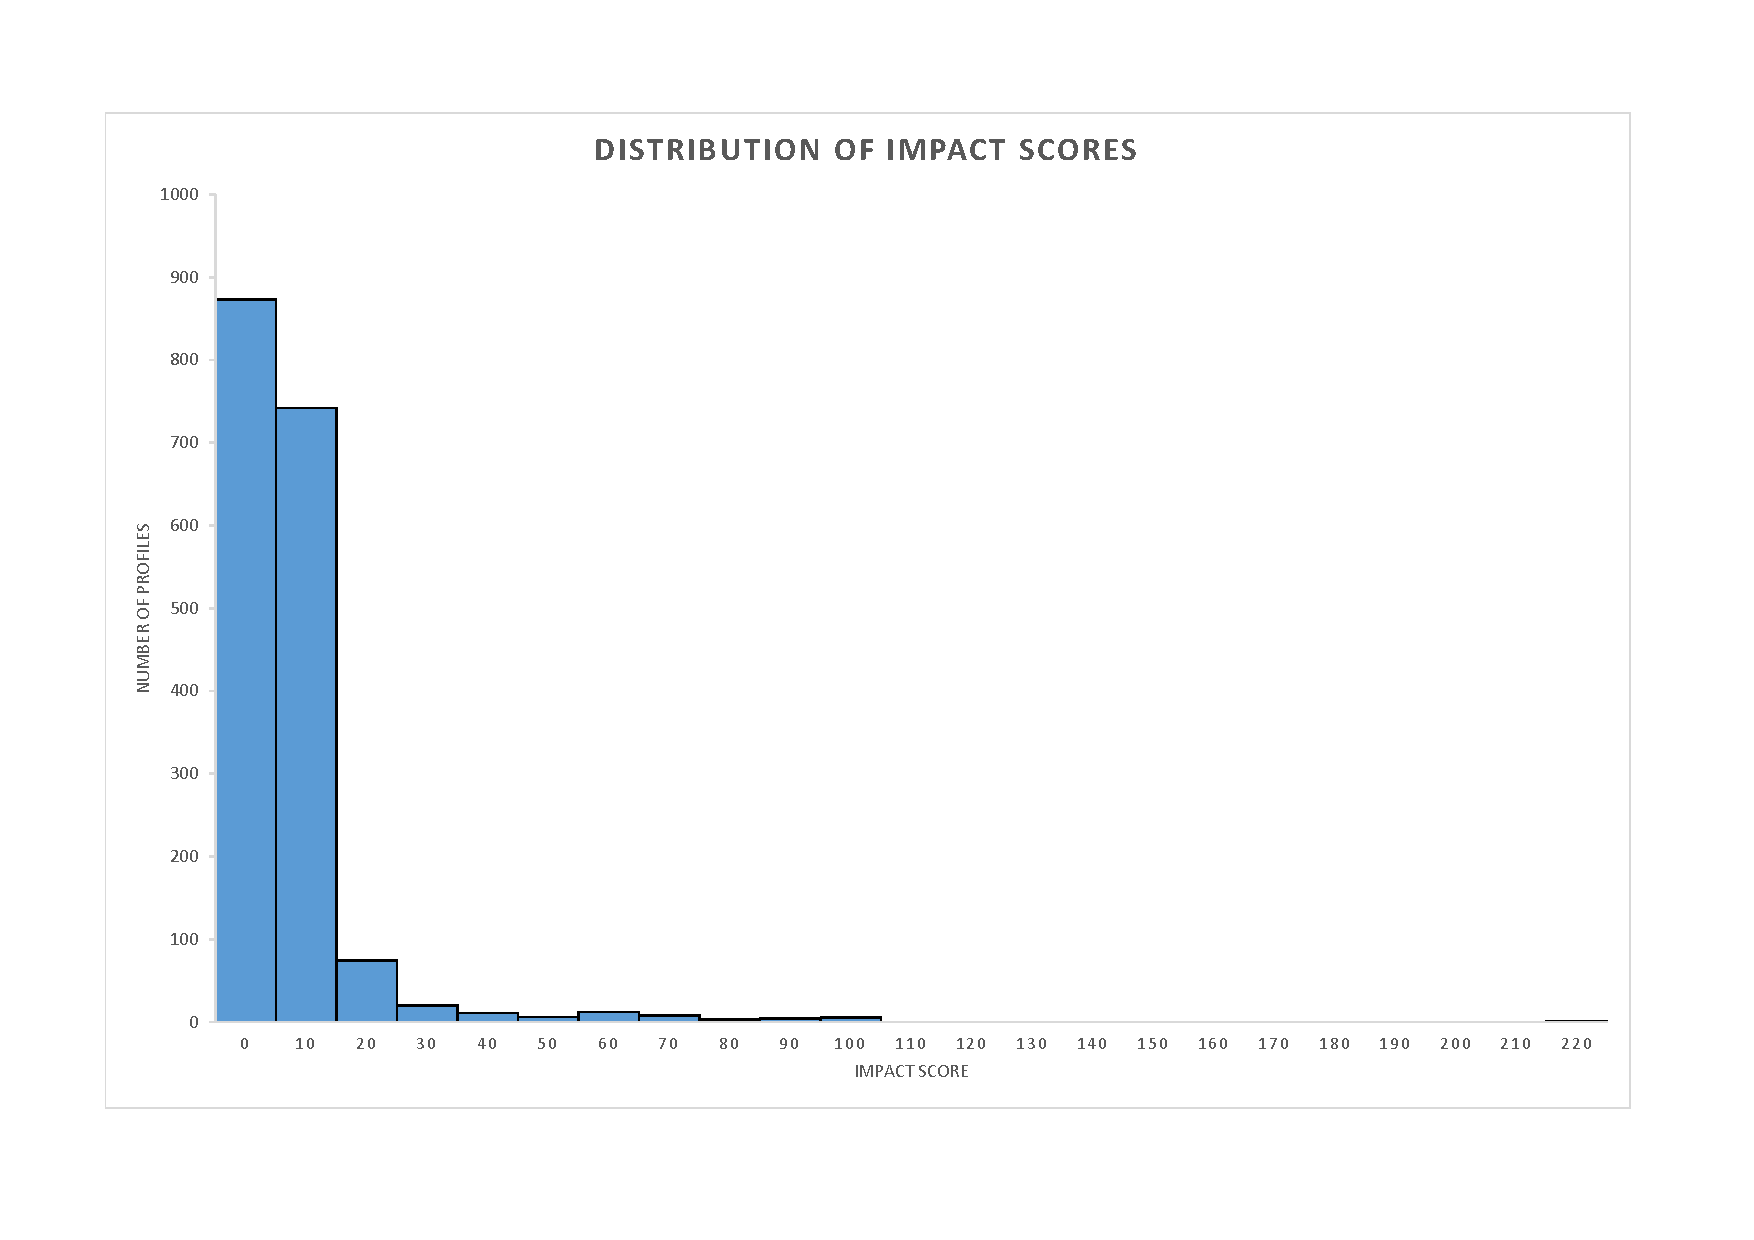
\includegraphics[width=500px]{Images/impact_distribution_histogram.pdf}
\caption{Distribution of Impact Score Among Users}
\label{fig:dist_impact_score}
\end{center}
\end{figure}

Figure \ref{fig:dist_impact_score} displays the distribution of impact factor values, over the set of twitter profiles collected. We can see that the impact score follows a roughly exponentially decreasing curve, with the vast majority of users getting a low impact score. This is reflective of past research, studying the behaviours of Twitter users \cite{beevolve}. That is, user patterns can be broken up into users who follow others and do not post much content themselves, and users who are more active and are followed by others. The extremely high impact scores are likely celebrities - the profile with the highest impact score of 216 was the Jonas Brothers (a pop band) profile, which happened to feature in the dataset. 

The impact factor calculation differs from other social media impact algorithms in that there is no upper limit on score. Other methods are arbitrarily capped at values like 10 or 100, which restricts the comparative value of such tools for the high echelons of impacting-users. The algorithm also automatically takes into account the length of time a user has been active on Twitter when performing the calculation. 

Extensions to the impact factor algorithm could include use of data such as number of followers, as well as frequency or consistency of posting. For example, users which have a large following but whom only have very low retweet counts may imply that content posted is somewhat stale. Also, an individual who had a strong impact in the past but who has not posted recently should logically receive a lower current impact; the current algorithm will not differentiate from an active user and an inactive one. This temporal structuring and analysis for a reputation policy is worth exploring further. 

\subsection{Temporal Clustering and Impact Factor}

In order to differentiate from \textit{one-hit-wonders} and \textit{constant emitters} in reputation policies, some view of activity over time was discussed. We refer to this as temporal clustering. One approach is to cluster impact score calculation into separate months. This reveals how consistently influential a person is, and gives the potential for detecting inactive users. Various bucket sizes were experimented with - days were much to varying to interpret a clear underlying trend, whilst years were too coarse to solve the issue of inactive users receiving a high impact score. Thus months are used as a bucketing measure.

\begin{figure}[h!]
\begin{center}
\centering
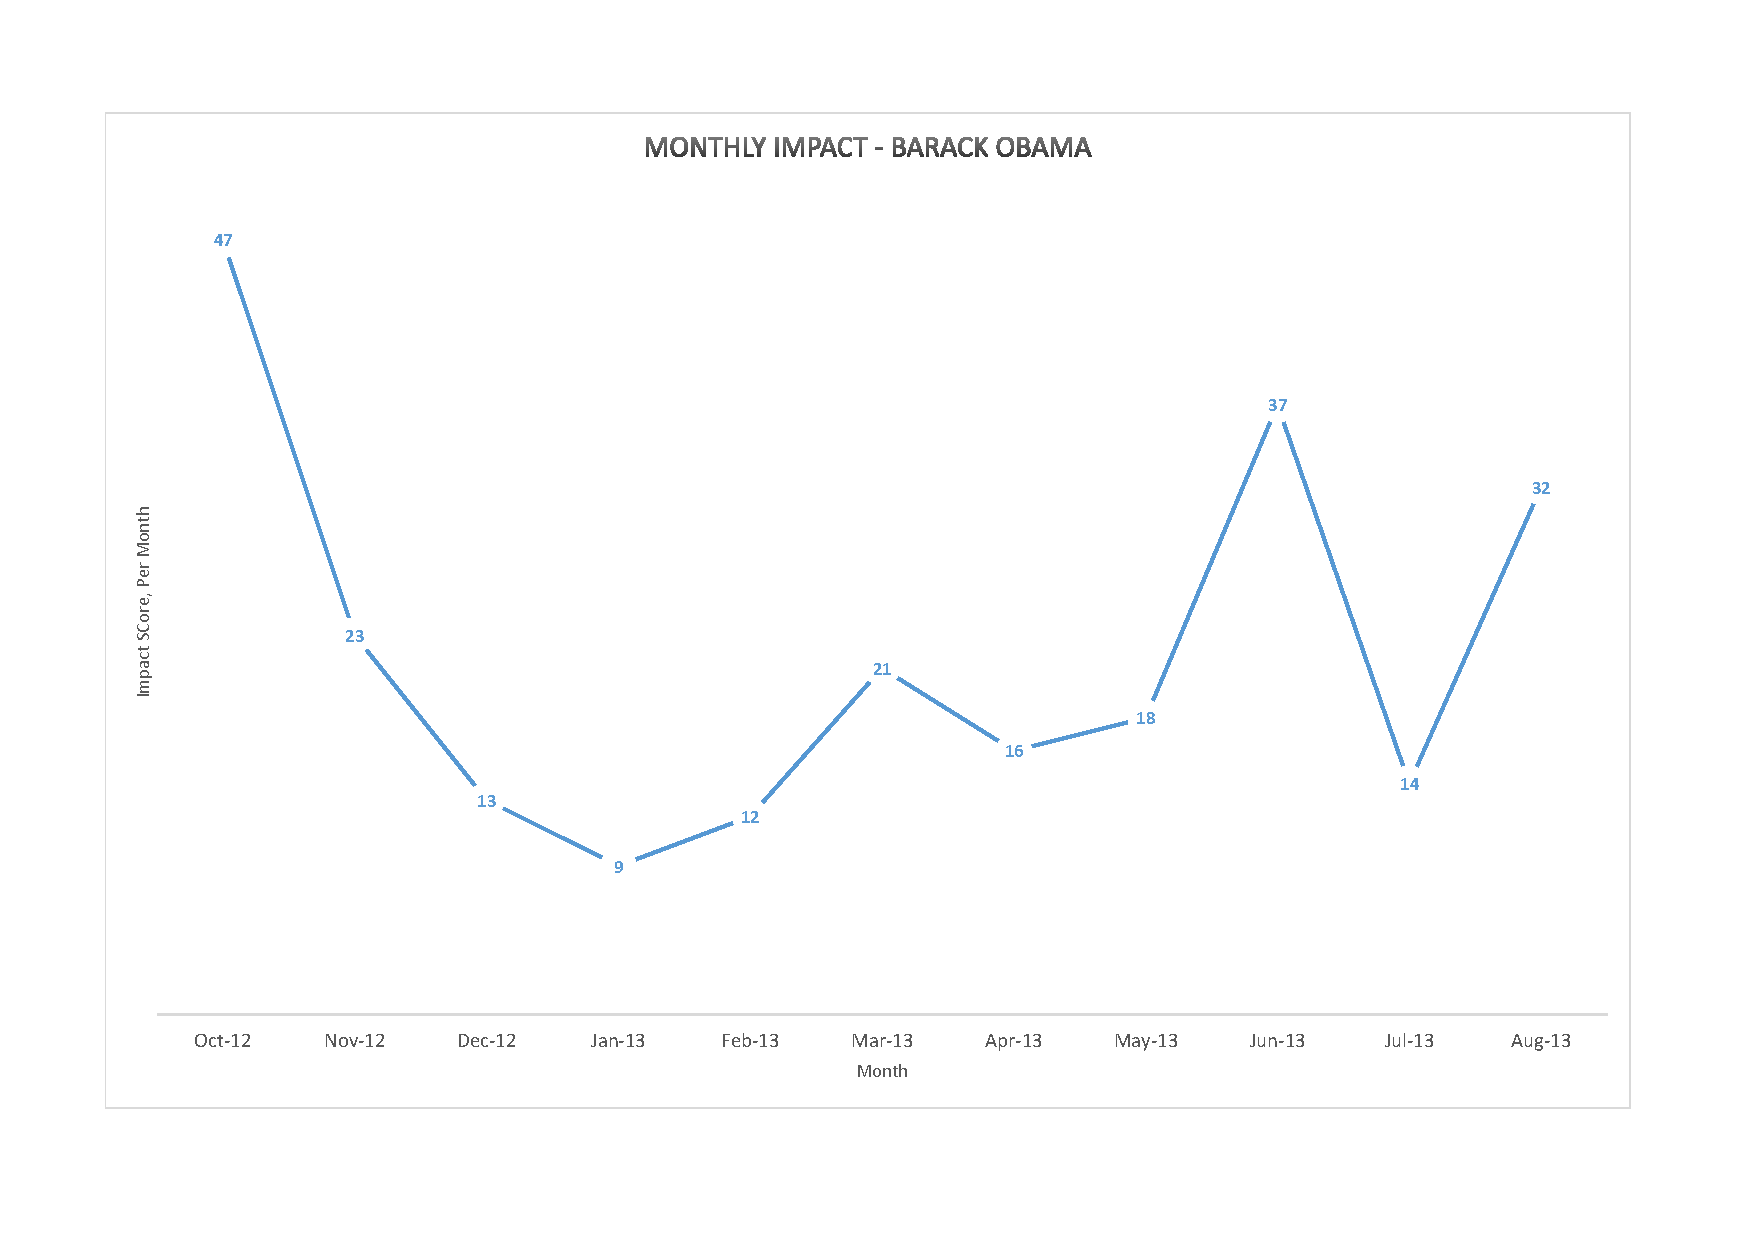
\includegraphics[width=500px]{Images/barack_obama_monthly_impact.pdf}
\caption{An Example of Monthly-Impact Score Bucketing - Barack Obama}
\label{fig:obama}
\end{center}
\end{figure}

This technique can be used to link real-world events to a person's influence. Barack Obama is taken as an example, as seen in Figure \ref{fig:obama}. In October and November of 2012, the US presidential elections were at their peak. The corresponding impact score of 47 for Obama in October is reflective of this. 

To demonstrate this on another individual, take Chris Hadfield (Twitter name Cmdr\_Hadfield), made famous through his cover of David Bowie's 'Space Oddity'. Figure \ref{fig:hadfield} shows how Hadfield's popularity spiked around the time of this video's explosion in popularity - June this year. 

\begin{figure}[h!]
\begin{center}
\centering
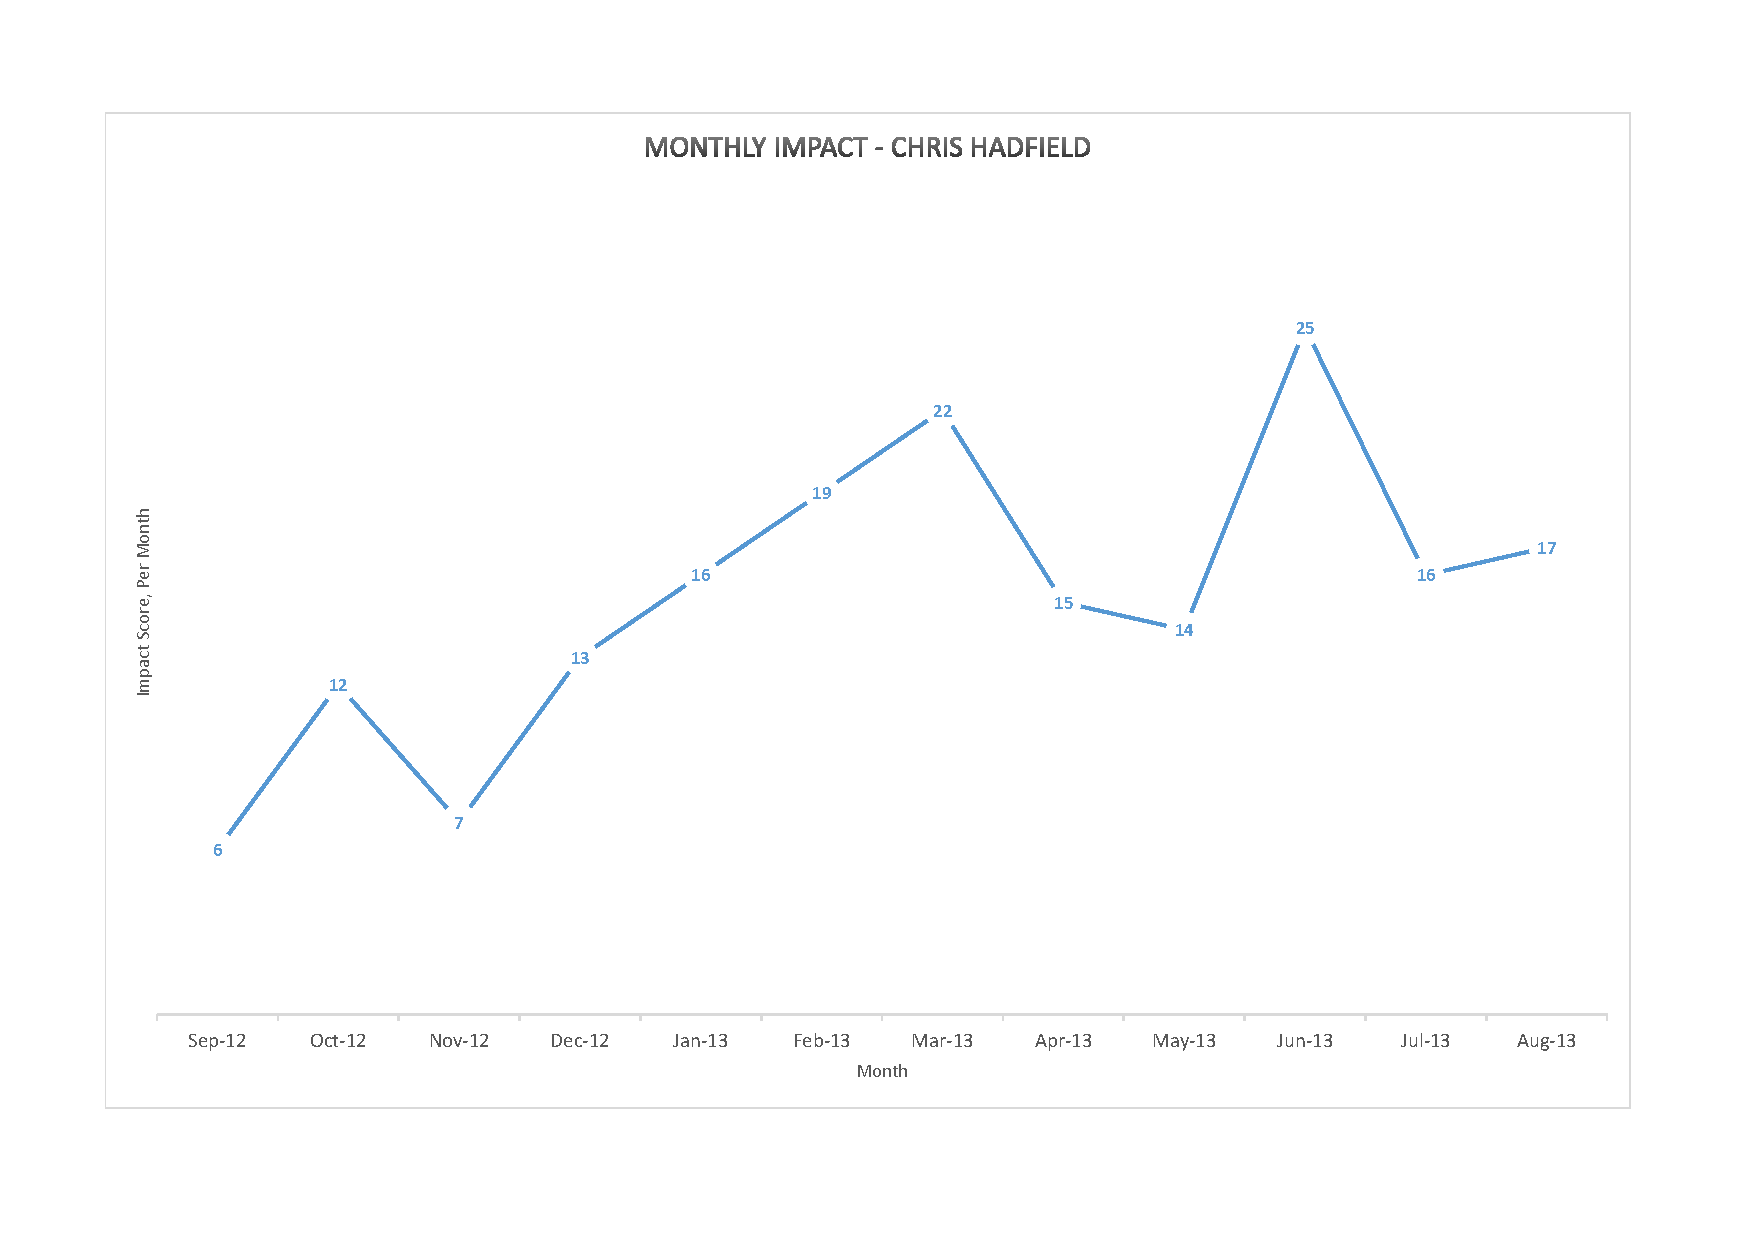
\includegraphics[width=500px]{Images/chris_hadfield_monthly_impact.pdf}
\caption{The Monthly Impact of Chris Hadfield - Famous Astronaut}
\label{fig:hadfield}
\end{center}
\end{figure}

\section{Community Detection}

The second primary data exploration factor explored community detection on Twitter. As a second hypothesis, we attempt to validate that embedded social networks exist within Twitter, and can be detected using IHPScrape. Detection of these communities will be possible through two means; follower and following links, and connection through retweets. Data collected for detecting communities consists of two sets to verify this claim; the retweet links, and follower links. These sets are largely disconnected, and as such discussion of these two techniques must also be separated.  
% 
% I propose the following. 
% 
% \begin{description}
% \item[H2.]{Embedded social networks exist within Twitter, and can be detected using IHPScrape. Detection of these communities will be possible through two means; follower and following links, and connection through retweets.}
% \end{description}



\subsection{MapEquation Tool}

MapEquation is a leading community-detection software tool, which uses graph-traversing techniques to detect the presence of sub-communities in a network \cite{mapequation}. In short, the algorithm aims to cluster neighbouring nodes into modules, then supermodules, and so on. Such an algorithm allows for a good clustering of a network in a very short time, and makes community detection feasible among millions of nodes.

The InfoMap software package distributed by mapequation is compatible with a Flash-based MapGenerator application, also hosted at the MapEquation site \footnote{http://www.mapequation.org/code.html}. This allows communities output through the InfoMap package to be visualised in a sensible manner. The following results were generated by gathering data, running community detection algorithms upon these sets, and visualising the results. Unfortunately the Flash tool is limited in terms of the numbers of nodes which may be loaded. My data consisted of millions of nodes and edges, and often the browser-based applet would cease functioning after data on the order of tens-of-thousands of nodes was loaded. The designers of the application are currently working on a newer version, to allow for larger quantities of data to be loaded through the MapGenerator tool, which would allow for more interesting community analysis in the future. 

\subsection{Followers and Following}

The first community detection approach considers those clustered around profiles, through links in following (profiles an individual is following) and followers (users who are following the current profile). I found that disconnected communities are clustered around popular figures. Figure \ref{fig:stevenadamsfollowers}, taken from Steven Adams profile, is a visualisation of the community formed through a subset of his followers. 

\begin{figure}[h!]
\begin{center}
\centering
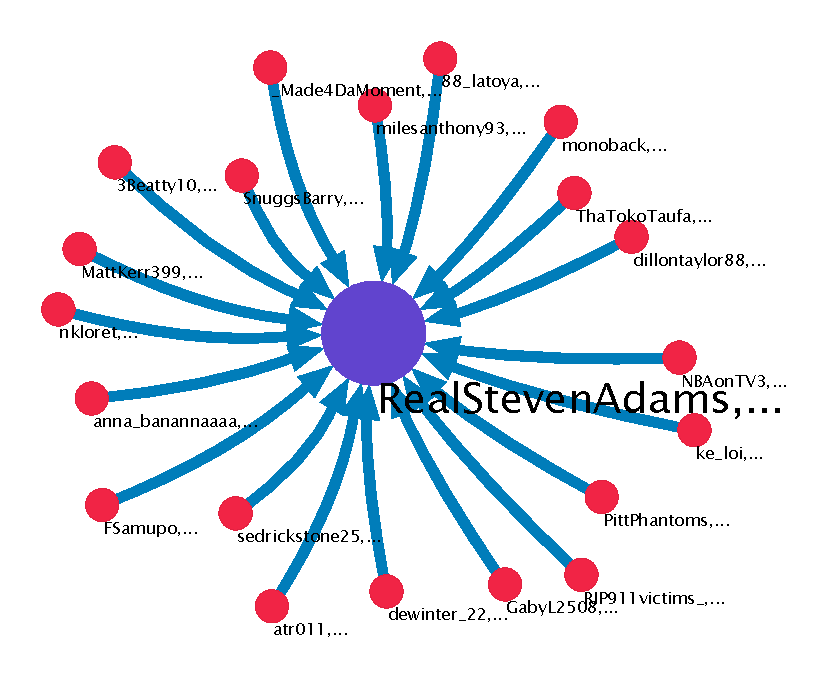
\includegraphics[width=300px]{Images/steven_adams_followers.pdf}
\caption{Followers of Steven Adams}
\label{fig:stevenadamsfollowers}
\end{center}
\end{figure}

% Unfortunately due to the limitations of the tool used, larger sets of data were not able to be loaded in this context. I feel that with more results, larger and connected communities would be evident through the follower and following connection on Twitter.

\subsection{Retweet Communities}

The second approach taken considers the communities formed on Twitter through retweeting of content. I consider two profiles to be connected if one retweets the other. This is ordered by the retweeter being connected to the original poster, respectively. Heavier weight is added to the connection if a user retweets posts from the user multiple times. As this retweet connection is richer, visualisations of communities formed are of more interesting structure. 

\begin{figure}[ht]
\centering
\begin{minipage}[b]{0.45\linewidth}
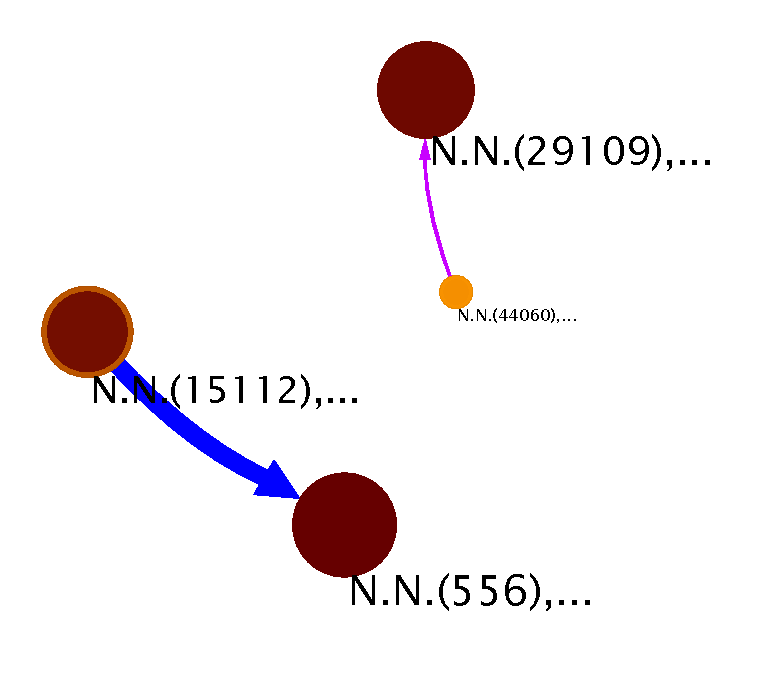
\includegraphics[scale=0.40]{Images/retweets_modules.pdf}
\caption{Retweet detected community modules}
\label{fig:minipage1}
\end{minipage}
\quad
\begin{minipage}[b]{0.45\linewidth}
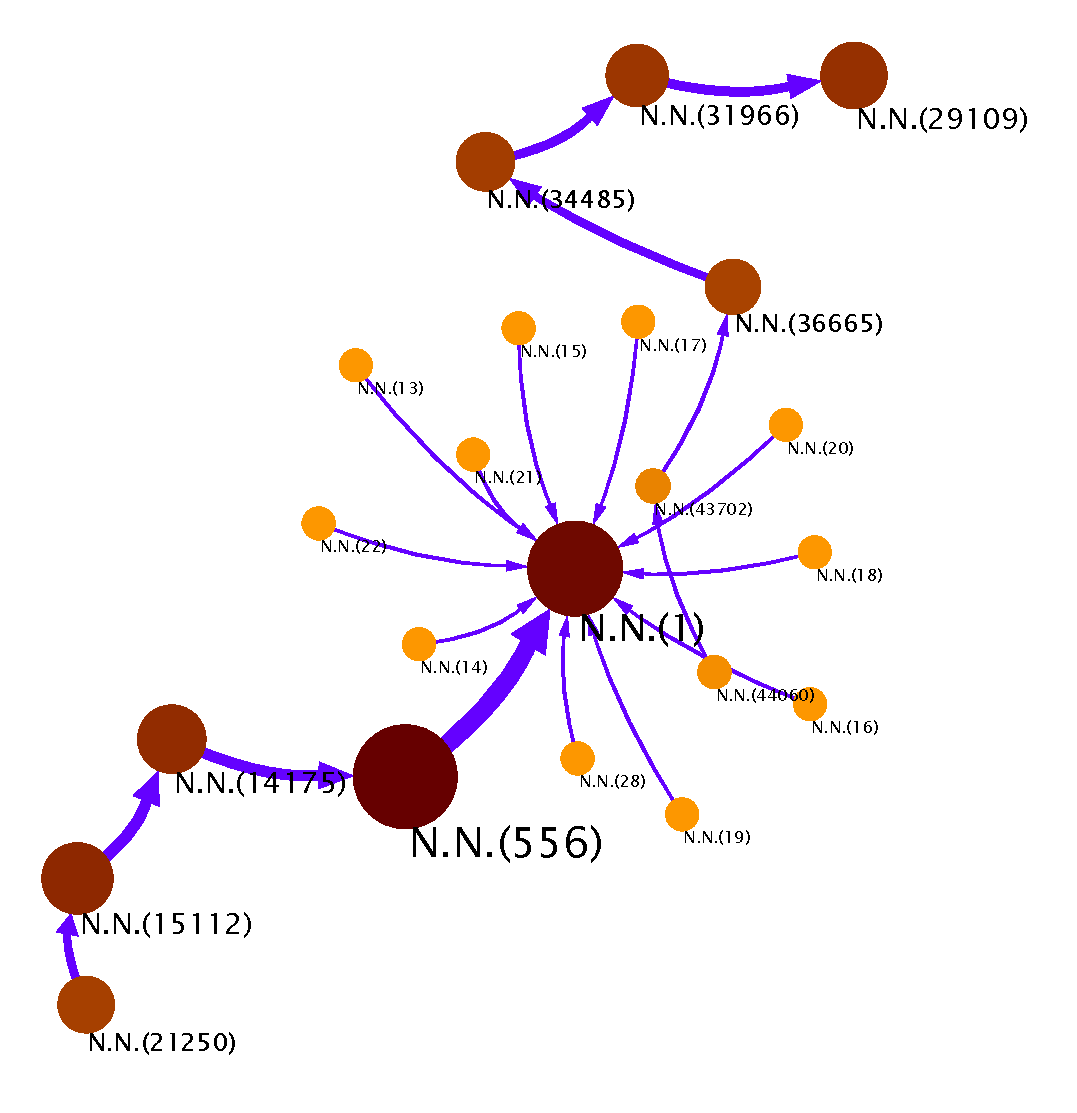
\includegraphics[scale=0.40]{Images/retweets_source_nodes.pdf}
\caption{Retweet source nodes}
\label{fig:minipage2}
\end{minipage}
\end{figure}

Unfortunately the MapGenerator tool did not allow for any entire set of profile and retweet data that was collected to be visualised in one piece. This is due to the extremely large quantity of nodes that are generated through the fetching of a single profile, and the entire collection of retweet or followers links associated with this profile. This largely reduced the use of current retweet communities, and the visualisation options for generating meaningful understanding of data collected, as arbitrary divisions in data necessary to be loaded into the tool introduce bias. Figures \ref{fig:minipage1} and \ref{fig:minipage2} are the retweet communities generated from the first quarter of one Twitter profile scraped. 

% as divisions in data were necessary to load into the tool introduce bias.

\subsection{Community Discussion}

The scrapers allowed for detection of communities for the two groups of followers and following, as well as detection of communities among retweeting circles. While the tools available certainly allowed for the detection of these communities, there is no way with the analysis tools currently provided to associate any real meaning with these groups. Future projects could assign meaning with the data that has been extracted - for example with sentiment or keyword classifying of tweet conversation topics for a profile. This would allow for meaningful classification of communities on Twitter, rather than simply grouping around profile names such as the grouping shown in Figure \ref{fig:stevenadamsfollowers}. This feature was left out of scope. Due to the large potential for extension of this community detection function, the policies ahead make assumptions on the classification of these groups being possible. 

%Positive outcomes of community detection - was able to group w.r.t to followers and following, as well as for retweeting communities.

%Limitations of community detection w.r.t. the connection between following/follower sets and the retweeter sets. Room left for development of components that are able to connect these sets. 

%Unfortunately limitations of the tools used to visualise and compute communities on Twitter, as well as scraping limitations resulted in 

%This investigation of community detection is not complete, and as such policies derived from community detection in this project are not entirely reflective of what I achieved. 

\subsection{Sentiment Analysis}

One avenue for enriching the community data would be to use sentiment-detection methods. Filip Dimitrievski's project was primarily focused on classifying social media posts based upon sentiment, and constructing policies based on this information. He was able to use data collected from the IHPScrape scrapers to classify tweets according to sentiment, with varying success with different classifiers such as Sentiment140\footnote{http://www.sentiment140.com/}. Although the classifier was not trained specifically to Twitter data and in the long run the approach was abandoned, this demonstrated the feasibility of such an approach. Future exploration of this is left to future work.

% Further exploration of this is left to future work, given that the project was not Artificial-Intelligence focused.

\section{Policy Examples and Discussion}

Reputation-inferring policies can be constructed from the data collected. Two exemplar policies are presented, which could be built as part of a system requiring reputation data related to a user's profile. These policies are applied in relation to a theoretical case study.

% I discuss 2 exemplar policies in particular which could be built as part of any system requiring reputation data related to a user's profile. I apply these policies in relation to a theoretical case study, that requires access policies based upon user reputation from an external source. 

\subsection{Case Study - Discussion Forum}

In order to introduce exemplar reputation policies, the concept of an interactive forum is used. This concept is inspired by Hendrikx at al. \cite{graft_paper}, where GRAft was applied to a social forum, using a pure reputation access control system. In this example, forum access control may be modified by restricting or granting additional rights to users based upon calculated reputation. Reputation is turned into access control rights by these policies.

As in the GRAft paper, I provide policy fragments, using Ruler\footnote{https://github.com/bobthecow/Ruler} to demonstrate how such a policy engine may operate. The following policy fragment restricts access based upon the impact factor of the given user, combined with the community that the individual is a part of. For example, on a computer science forum the administrator may only desire users with a significant social media impact to do with the engineering discipline to be able to post. In the example the calculated impact factor of the user is enfored to be greater than or equal to 1, and the computed community discipline is related to the current forum, in order to post. 

% Here I propose that the calculated impact factor of the user is greater than or equal to 1, and the computed community discipline is related to the current forum, in order to post. 

\begin{center}
 \textbf{Policy 1: Impact Factor and Community Participation}
\begin{verbatim} 
 $rb->logicalAnd(
  $rb['impact_factor'] -> greaterThanOrEqualTo(1),
  $rb['community_value'] -> in_array(['computer_science','engineering'])
 ) 
\end{verbatim}
\end{center}

Whereas for read-only rights, the person may only need to be part of the relevant discipline.

\begin{verbatim}
 $rb['community_value'] -> in_array(['computer_science','engineering'])
\end{verbatim}

On the same forum, administrator rights may be granted to consistently active users. Some evidence of consistent activity on social media might be required for effective administration of the site. In this exemplar policy, administration rights are granted to the user if their average monthly computed impact is greater than or equal to 3, and they are part of the computer science or engineering community. 

\begin{center}
 \textbf{Policy 2: Impact Factor, Community Participation and Temporal Consistency}
 \begin{verbatim}
   $rb->logicalAnd(
    $rb['temporal_impact_average'] -> greaterThanOrEqualTo(3),
    $rb['community_value'] -> in_array(['computer_science','engineering'])
  ) 
 \end{verbatim}
\end{center}


%Performance

%Resistance to Detection

%Logging


%Our definition of equivalent defines that 

%\section{Temporal Clustering}

%By looking at impact across a period of time, we are able to distinguish constant emitters from one-hit-wonders, who 

%\subsection{Correlation of Impact Factor vs Bucketed Impacts}

%\begin{figure}[h!]
%\centering
%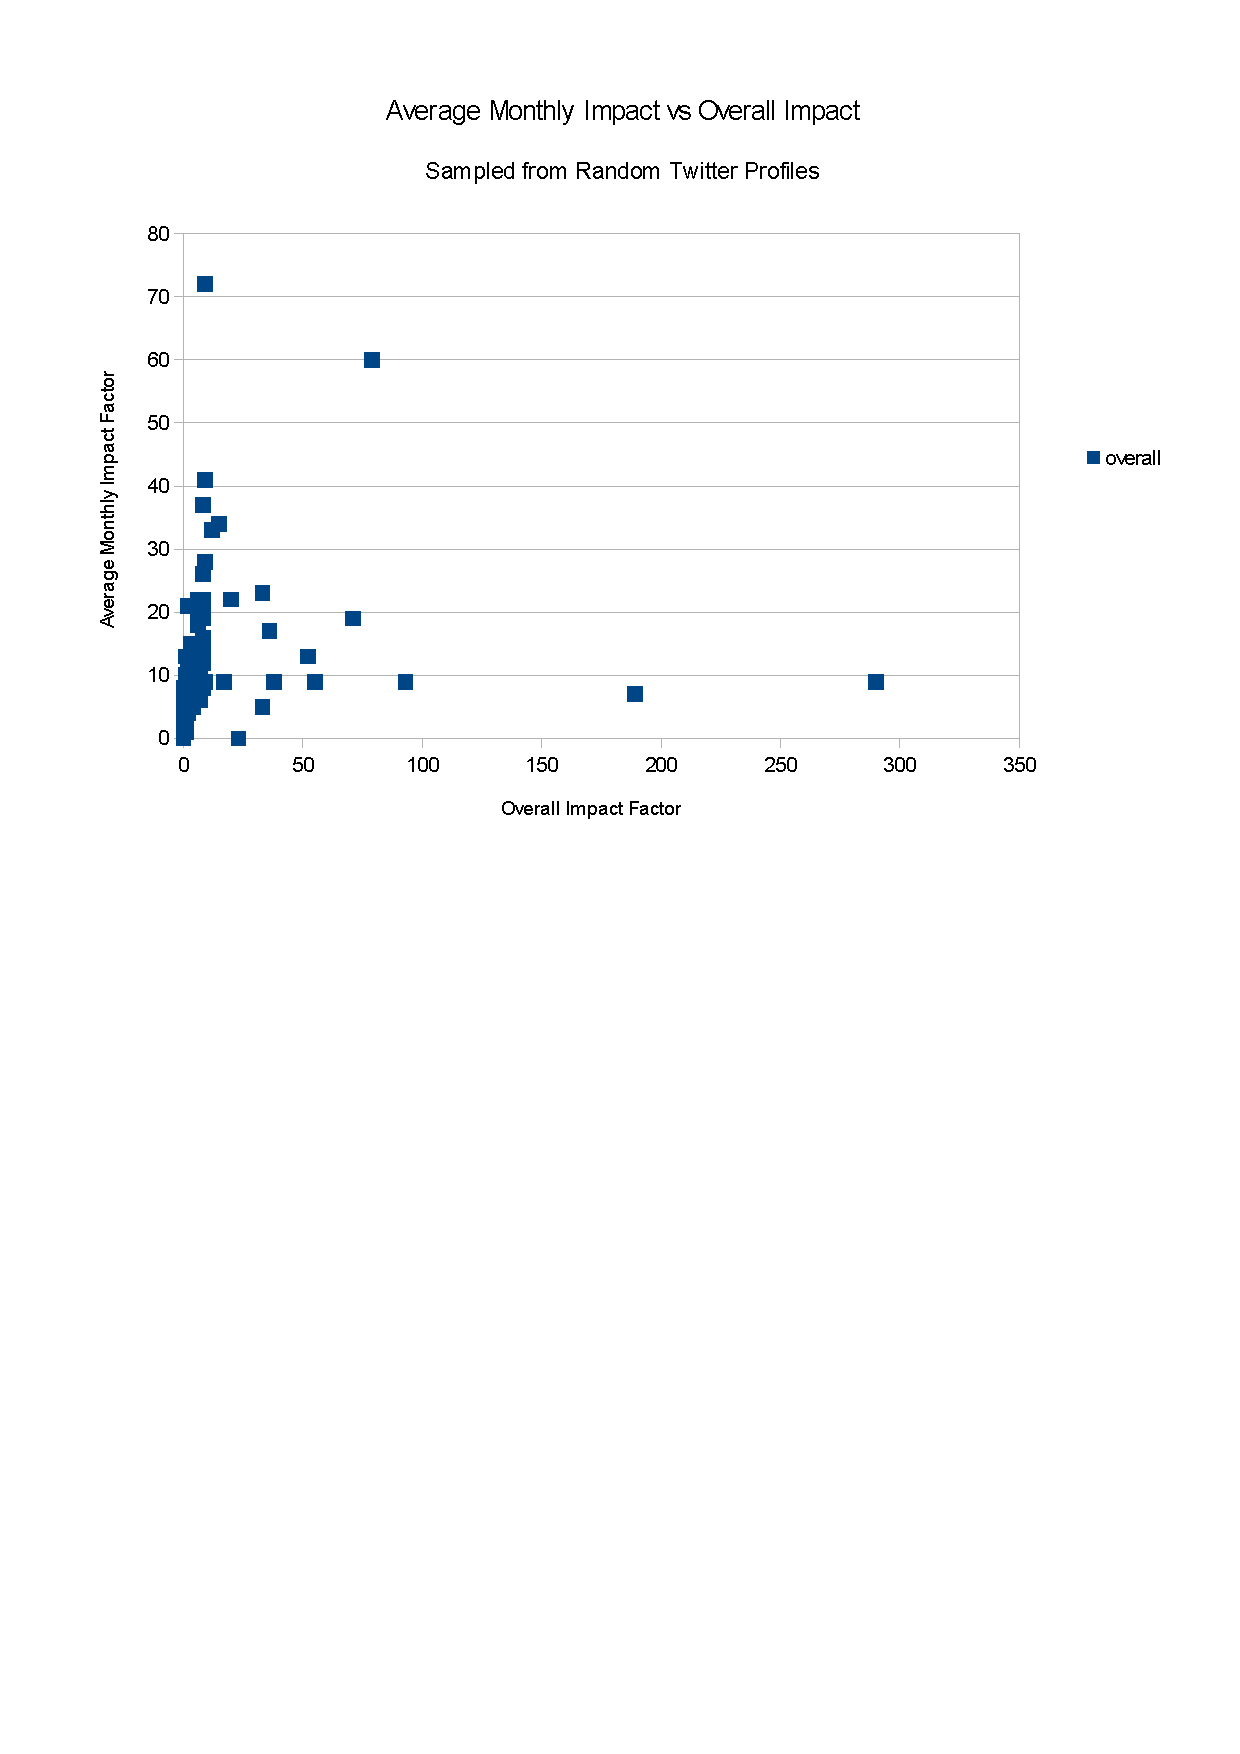
\includegraphics[width=400px]{Images/monthly_impact_vs_overallv2.pdf}
%\caption{Monthly Impact against Overall Impact}
%\end{figure}

%\begin{figure}[h!]
%\centering
%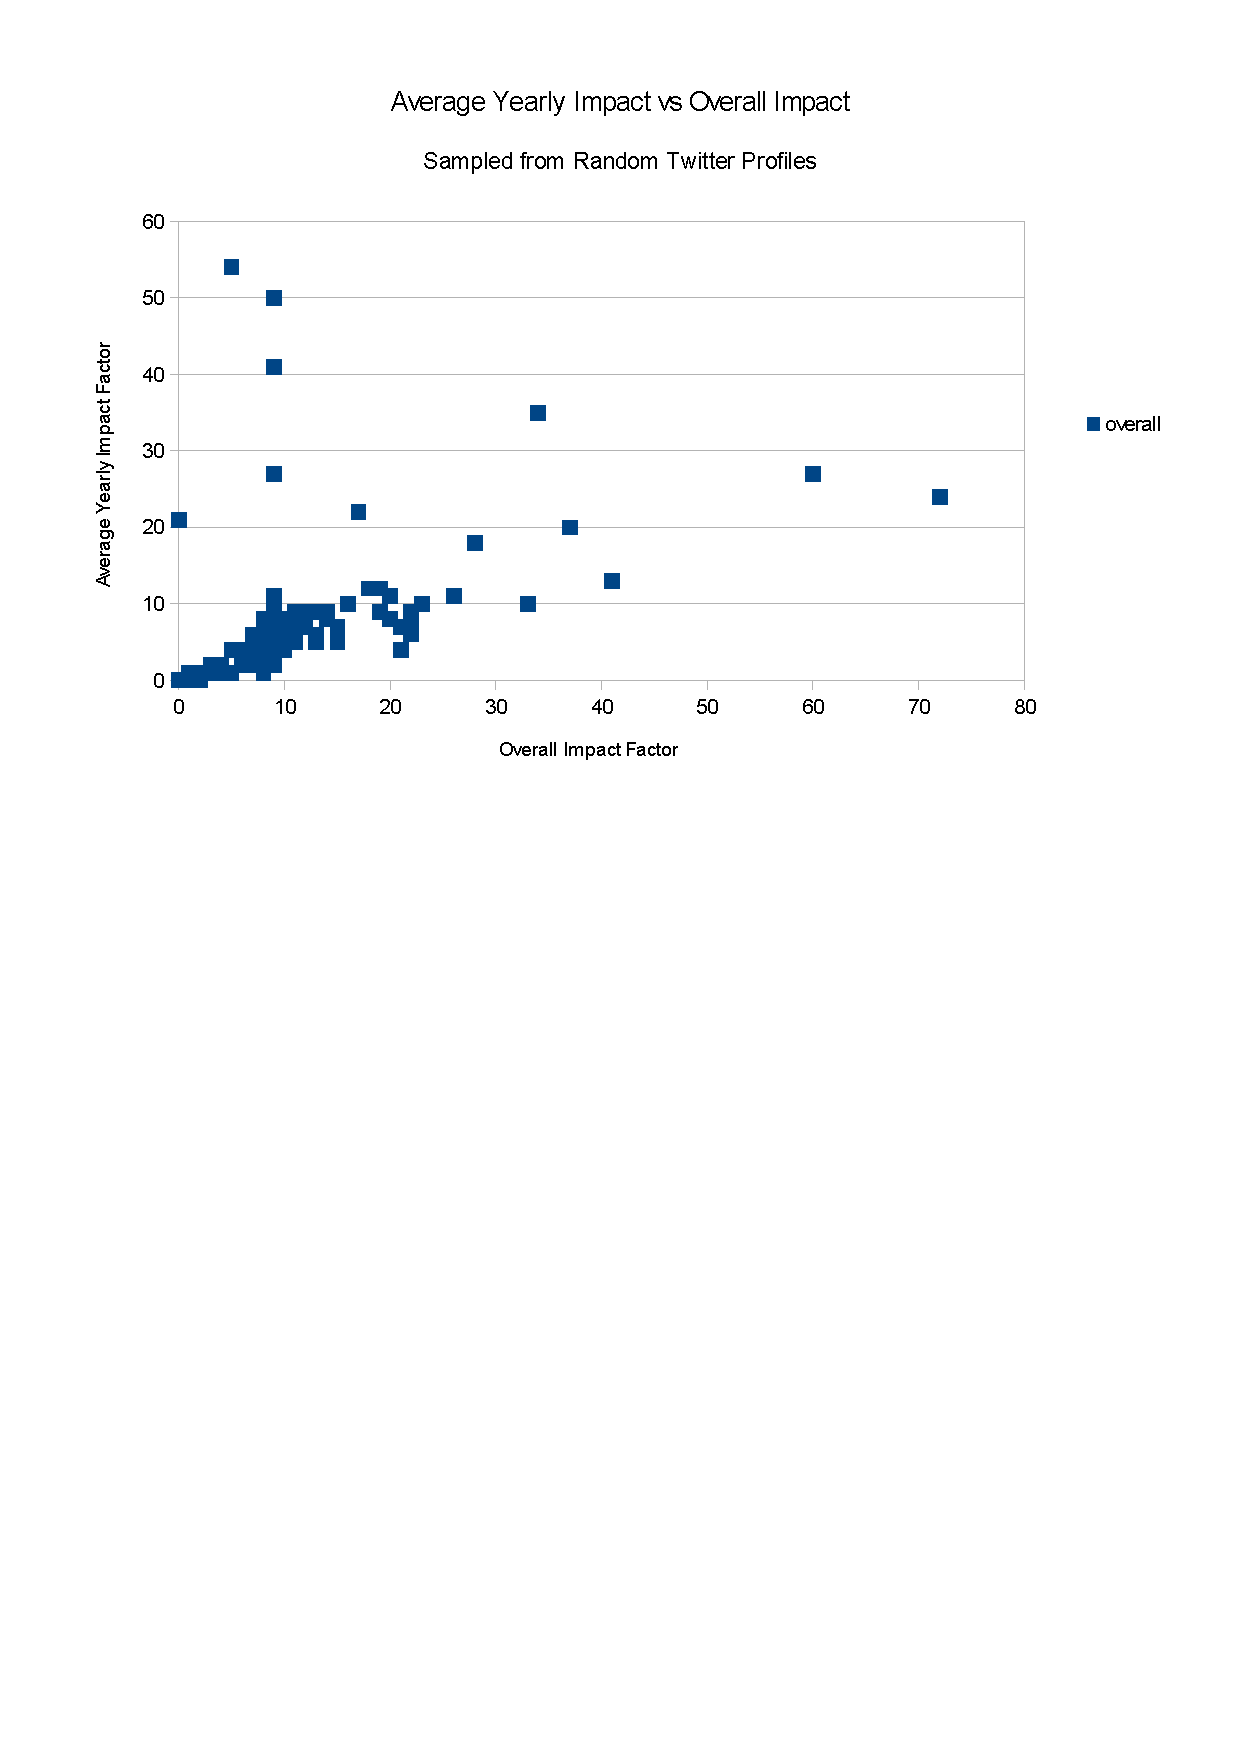
\includegraphics[width=400px]{Images/yearly_impact_vs_overallv2.pdf}
%\caption{Yearly Impact against Overall Impact}
%\end{figure}

%One strategy for inferring reputation information that I looked at was through temporal bucketing of impact factor, into days, months, and years. The figures below show the relationship between people's mean monthly calculated impact factor (i.e. by calculating a person's impact score for each month, and then averaging these values over the total number of months), and the individual's overall impact score. I infer that there is a weak relationship between average monthly impact and overall impact (Pearson's correlation coefficient of 0.273(3 s.f.)), and a stronger relationship between average yearly impact and overall impact (r=0.689(3 s.f.))\\

%\noindent What I believe this data shows is that the impact factor is favourable to individuals who are consistent on Twitter over time. 

%\subsection{Results of Monthly Bucketing}

%By applying the impact factor formula to individuals on a monthly basis, we are able to generate an impression of how regularly active a person is. The data also reveals how influential the person has been per month. This assists when comparing individuals who are consistently strongly influential (e.g. Barack Obama, companies such as instagram), with those who are popular for a limited period only. I looked at comparing different bucket sizes for this temporal aggregation. Days, months, and years were used as buckets, with monthly aggregation clearly showing the strongest and more interesting trends. 

%\begin{figure}[h!]
%\centering
%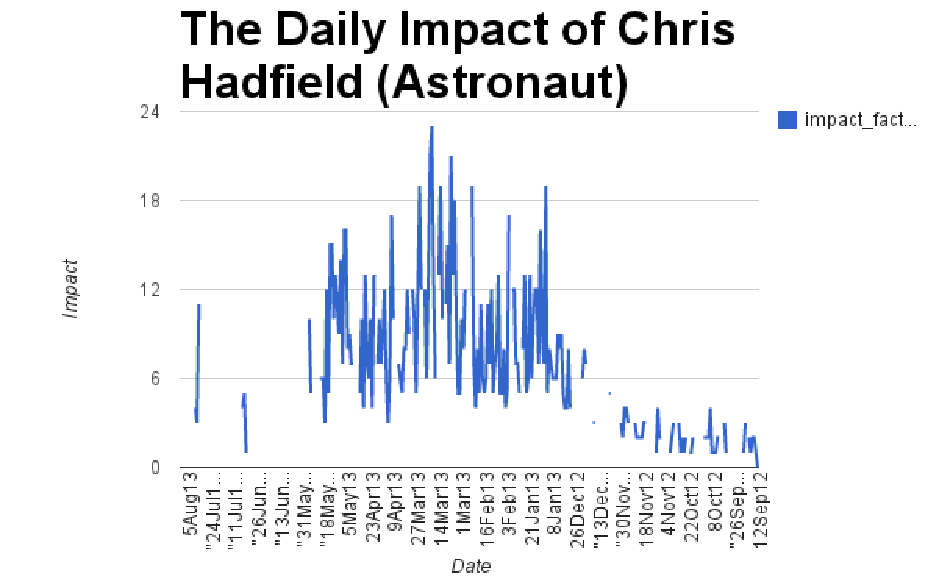
\includegraphics{Images/daily_impact_chris_hadfield.pdf}
%\caption{The Daily Impact of Chris Hadfield - Famous Astronaut}
%\end{figure}



%\begin{figure}[h!]
%\centering
%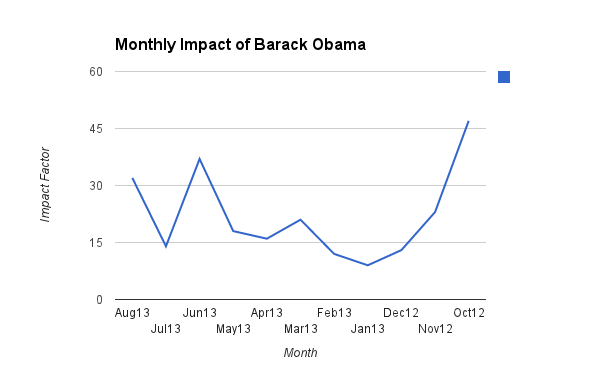
\includegraphics{Images/monthly_impact_barack_obama.png}
%\caption{The Monthly Impact of Barack Obama - President of USA (As if you didn't know that)}
%\end{figure}

%We can see that the daily and monthly impact trends follow roughly the same curve, which should be expected. The difference is due to the strictness of the impact factor formula in classifying someone as 'influential'. It is very difficult to get a value much above 1 on a daily basis, unless you are very frequently both making use of the social media, and having people respond to this activity. 


%\section{Monthly Bucketing of Impact}

%\section{Community Detection}

%\begin{description}
% \item [H2.] Sub-communities exist on Twitter, and we are able to detect these through scraping mechanisms.
%\end{description}



%One strategy for inferring reputation information that I looked at was through temporal bucketing of impact factor, into days, months, and years. The figures below show the relationship between people's mean monthly calculated impact factor (i.e. by calculating a person's impact score for each month, and then averaging these values over the total number of months), and the individual's overall impact score. I infer that there is a weak relationship between average monthly impact and overall impact (Pearson's correlation coefficient of 0.273(3 s.f.)), and a stronger relationship between average yearly impact and overall impact (r=0.689(3 s.f.))\\

%First present the use of retweets vs favourites on Twitter, and show that they are similar

%Next we look at impact factor of a person's retweets, pulled from the Hirsch-index formula. 

%Policies as an outcome of this, written using Ruler?
\chapter{Policy Evaluation}\label{C:us}


%\chapter{Evaluation}\label{C:us}

This section outlines my evaluation strategies, tests performed, and presents and discusses the results of evaluation conducted on the developed web scrapers. It then presents an evaluation of the policies and hypotheses formulated during analysis of data gathered. 

\section{Web Scraper Evaluation}

Performance - what performance goals did I have. How did they improve over time. Justify use of the incremental prototype-based strategy, through performance gains throughout the project.

Resistance to Detection - what performance goals did I have.

Problems

Accuracy - issues and why. Aims that I had - don't think I achieved them. In general entire profiles were not scraped. 



%Performance

%Resistance to Detection

%Logging



\section{Policy Evaluation}

This section outlines my evaluation strategies, tests performed, and presents and discusses the results of evaluation conduceted on the developed system. 

In order to evaluate my solution I need to refer back to the requirements gathered at the beginning of the project. 

- These requirements will be moved to the Requirements Analysis section... is just useful to have them stored here for easy referrals. 

\begin{itemize}
\item Develop a set of Policies that can be used to ...
\item Develop a metric of reliability of information gathered, based on privacy settings.
\item Potential to Develop an Interface with Filip Dimitrievski's project. Re-using my web-scraping libraries could be useful for his project. (Probably not going to happen)
\item Aggregate data for storage into GRAft
\end{itemize}

Non-Functional Requirements:
\begin{itemize}
\item Privacy Protection
\item Maintainability and Resistance to User-Interface Changes
\item Performance of Scrapers
\item Ability to Resist Blocking Detection, and Recover from Failure
\end{itemize}

\section{Policies}

\subsection{Correlation of Impact Factor vs Bucketed Impacts}

\begin{figure}[h!]
\centering
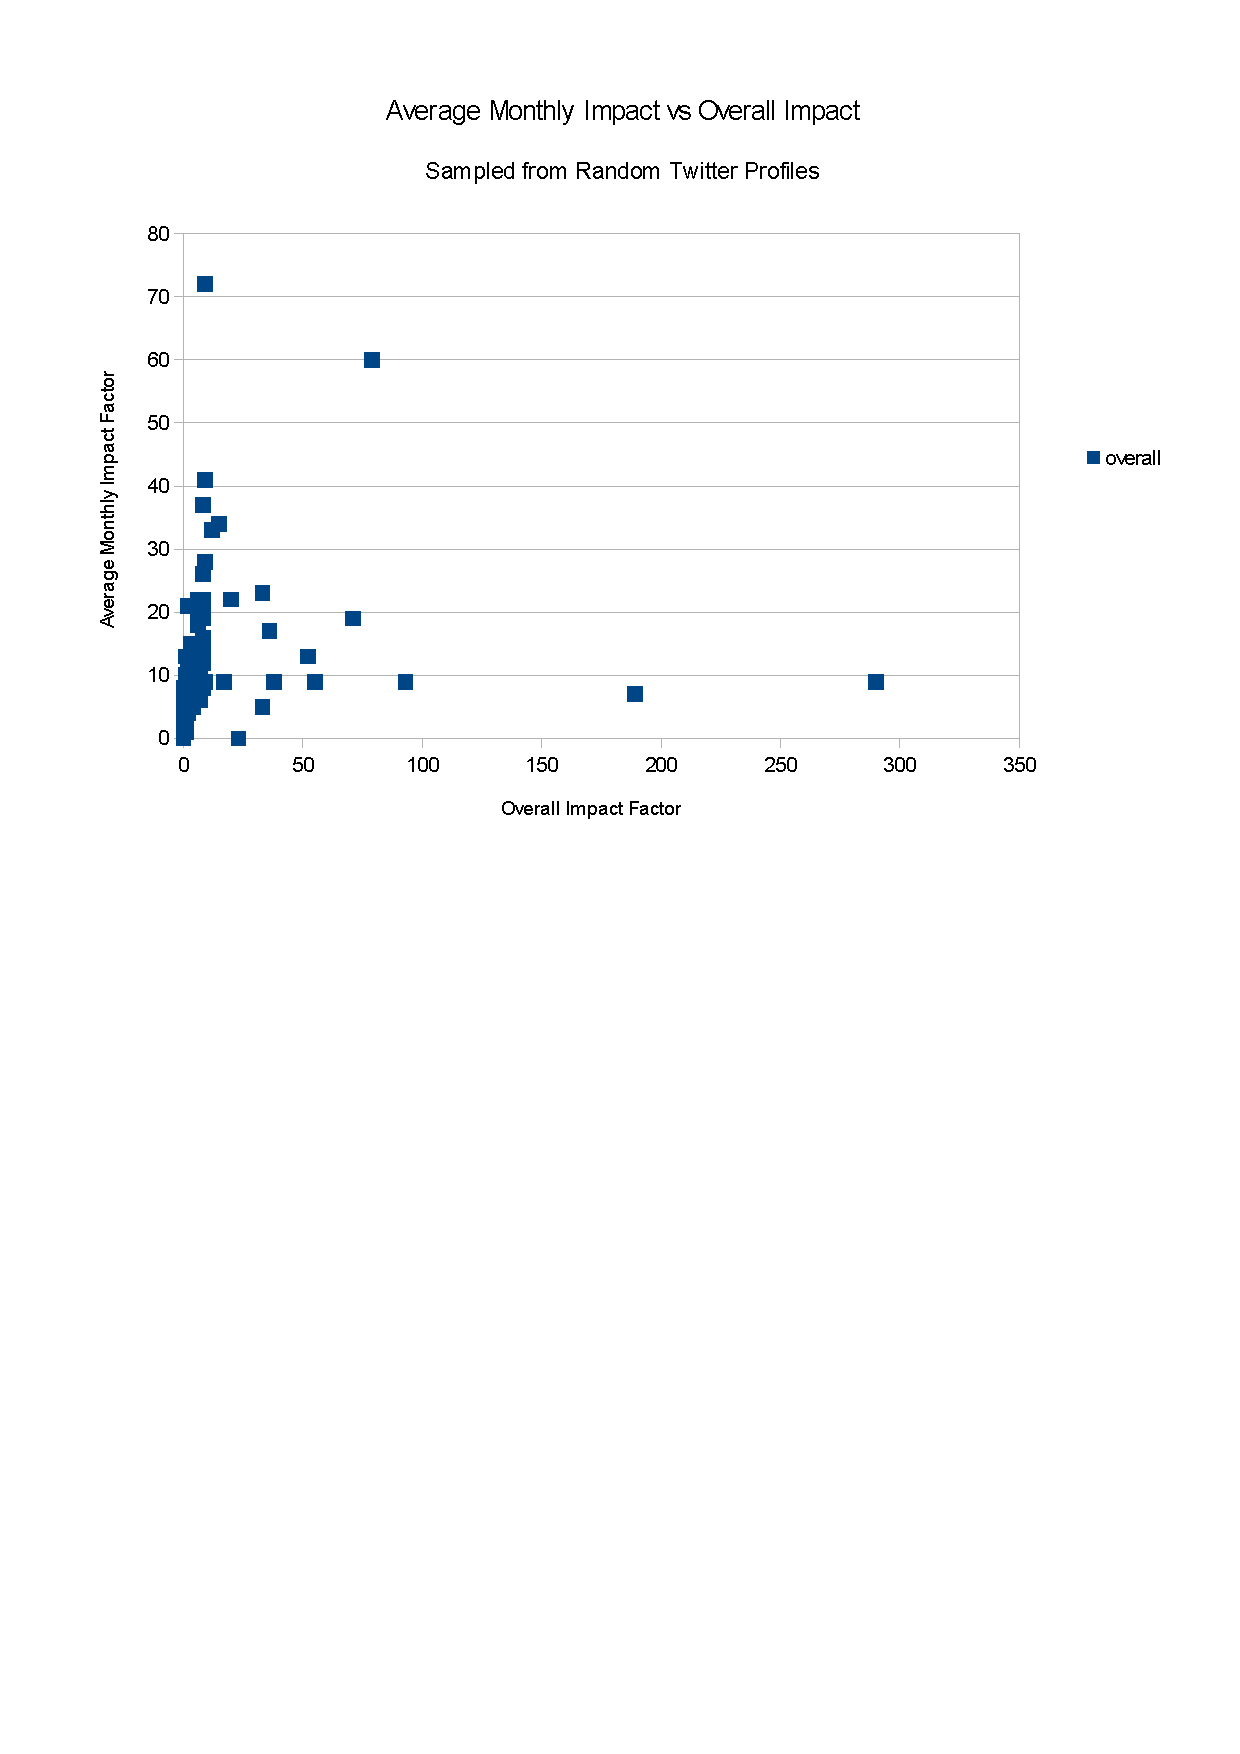
\includegraphics[width=400px]{Images/monthly_impact_vs_overallv2.pdf}
\caption{Monthly Impact against Overall Impact}
\end{figure}

\begin{figure}[h!]
\centering
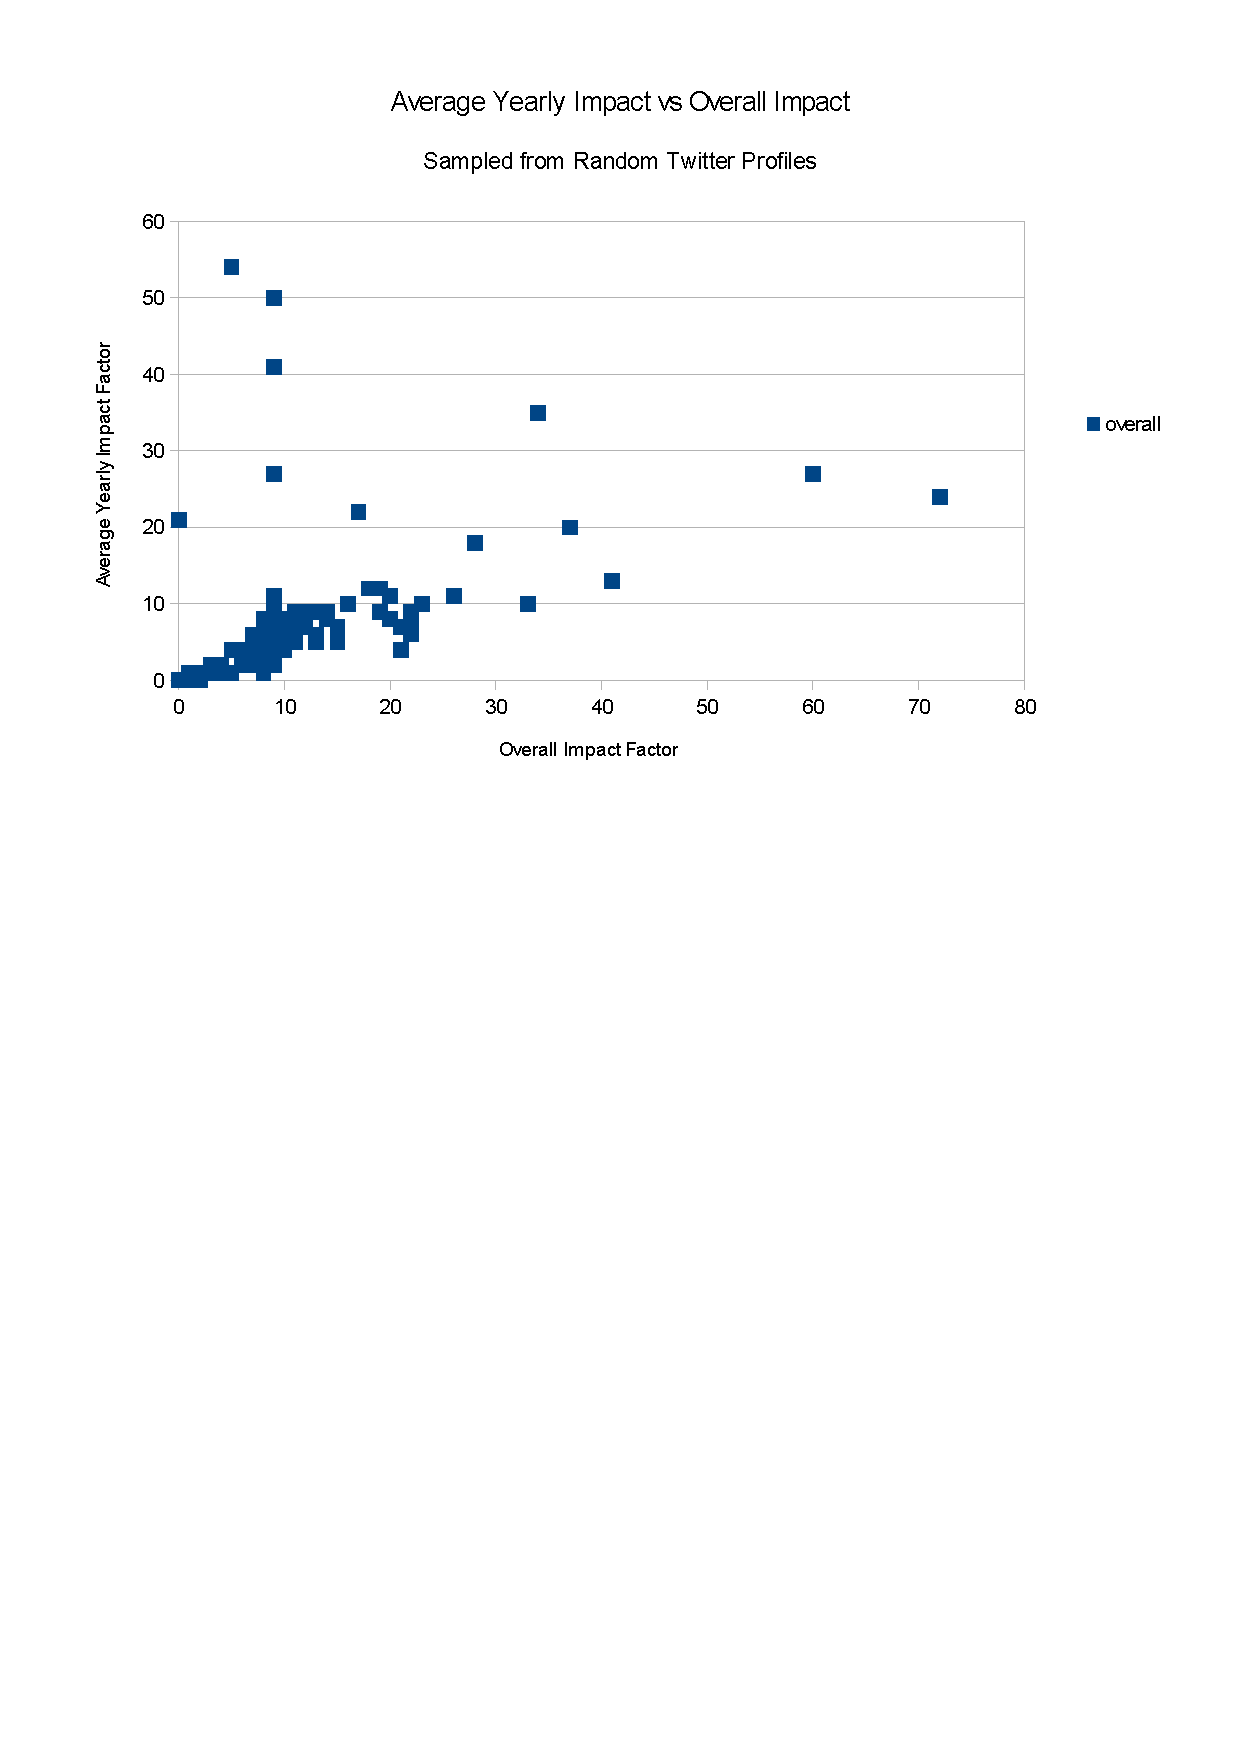
\includegraphics[width=400px]{Images/yearly_impact_vs_overallv2.pdf}
\caption{Yearly Impact against Overall Impact}
\end{figure}

One strategy for inferring reputation information that I looked at was through temporal bucketing of impact factor, into days, months, and years. The figures below show the relationship between people's mean monthly calculated impact factor (i.e. by calculating a person's impact score for each month, and then averaging these values over the total number of months), and the individual's overall impact score. I infer that there is a weak relationship between average monthly impact and overall impact (Pearson's correlation coefficient of 0.273(3 s.f.)), and a stronger relationship between average yearly impact and overall impact (r=0.689(3 s.f.))\\

\noindent What I believe this data shows is that the impact factor is favourable to individuals who are consistent on Twitter over time. 

\subsection{Results of Monthly Bucketing}

By applying the impact factor formula to individuals on a monthly basis, we are able to generate an impression of how regularly active a person is. The data also reveals how influential the person has been per month. This assists when comparing individuals who are consistently strongly influential (e.g. Barack Obama, companies such as instagram), with those who are popular for a limited period only. I looked at comparing different bucket sizes for this temporal aggregation. Days, months, and years were used as buckets, with monthly aggregation clearly showing the strongest and more interesting trends. 

\begin{figure}[h!]
\centering
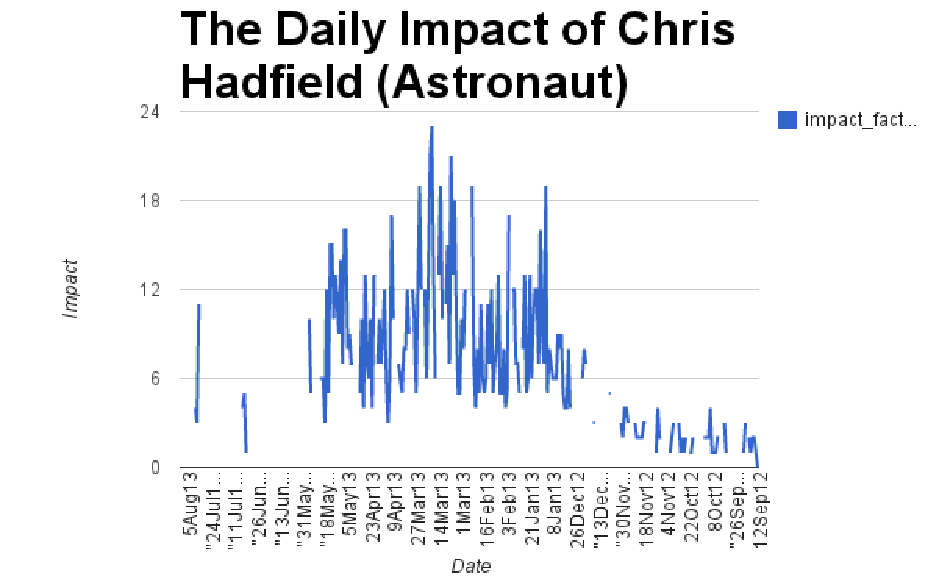
\includegraphics{Images/daily_impact_chris_hadfield.pdf}
\caption{The Daily Impact of Chris Hadfield - Famous Astronaut}
\end{figure}

\begin{figure}[h!]
\centering
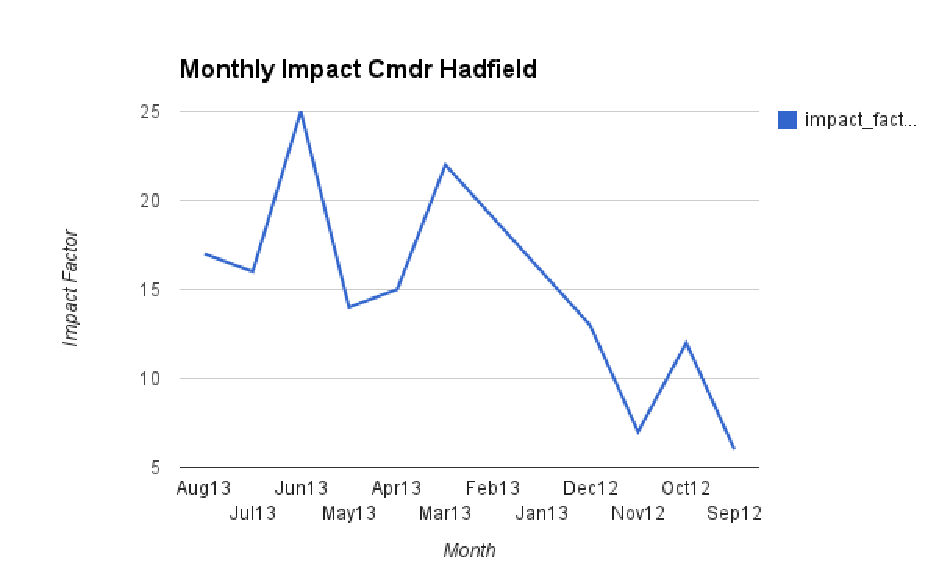
\includegraphics{Images/monthly_impact_chris_hadfield.pdf}
\caption{The Monthly Impact of Chris Hadfield - Famous Astronaut}
\end{figure}

\begin{figure}[h!]
\centering
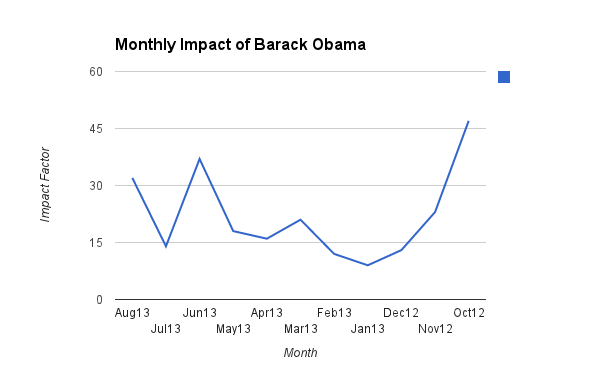
\includegraphics{Images/monthly_impact_barack_obama.png}
\caption{The Monthly Impact of Barack Obama - President of USA (As if you didn't know that)}
\end{figure}

We can see that the daily and monthly impact trends follow roughly the same curve, which should be expected. The difference is due to the strictness of the impact factor formula in classifying someone as 'influential'. It is very difficult to get a value much above 1 on a daily basis, unless you are very frequently both making use of the social media, and having people respond to this activity. 

\section{Scraper}

\subsection{Functional Requirements}

Aggregate data for storage into Graft - given that I am currently only storing data from Twitter this requirement has not yet been met.

Develop a metric of reliability of information gathered, based on privacy settings. Currently on Twitter there are two degrees of privacy - Open and Closed! Closed profiles means I cannot get any meaningful information, whereas on Open profiles I can get anything I want! Most profiles are open so this is not a concern. Profiles of celebrities etc are always set to open.

Developing a set of Policies - still in the production line, still experimenting with different ways of using the data.

\subsection{Non-Functional Requirements}

\subsubsection{Maintainability and Resistance of Scrapers to User Interface Change}
This is difficult to evaluate. Experiment: Change the layout of twitter pages, see how the scrapers react to these changes. How many changes do I need to make? There will undoubtedlu be single points of faiure, which I should mention. Important point: used as little xpath expressions as possible, as these inherently result in less flexbile scrapers. Any structural changes, or even a tag changing result in an xpath expression having to change. Still resistant to stylesheet changes, though.
Single points of failure.

\subsubsection{Twitter Scraper Performance}
I evaluate the performance of my twitter scraper with respect to average time taken to fetch and parse a tweet. The major limiting factor for scraping twitter was that each tweet had to be fetched with a seperate http request. Figure <x> shows the average time taken to fetch and parse each tweet, with respect to my incremental build stages. The success of continuous and incremental improvement in performance helps justify my decision to use an incremental approach. Tweets were gathered over several days, and continuously throughout different times of the day on the Victoria network to ensure that a representative range of times were gathered for each stage. 


I evaluate the performance of my twitter scraper with respect to average time taken to fetch and parse a tweet. The major limiting factor for scraping twitter was that each tweet had to be scraped with a seperate http request. Figure <x> shows the average time taken to fetch and parse each tweet, with respect to incremental builds. This also helps justify my incremental development strategy - we can see that succesive builds gradually increase performance. Tweets were gathered over several days, and at different times of the day on the Victoria network to ensure that a representative range of network performance speeds were used to gather data.\\

\noindent The significant feature of improved performance was through parellization of tweet-fetches. 

\begin{figure}[h!]
\centering
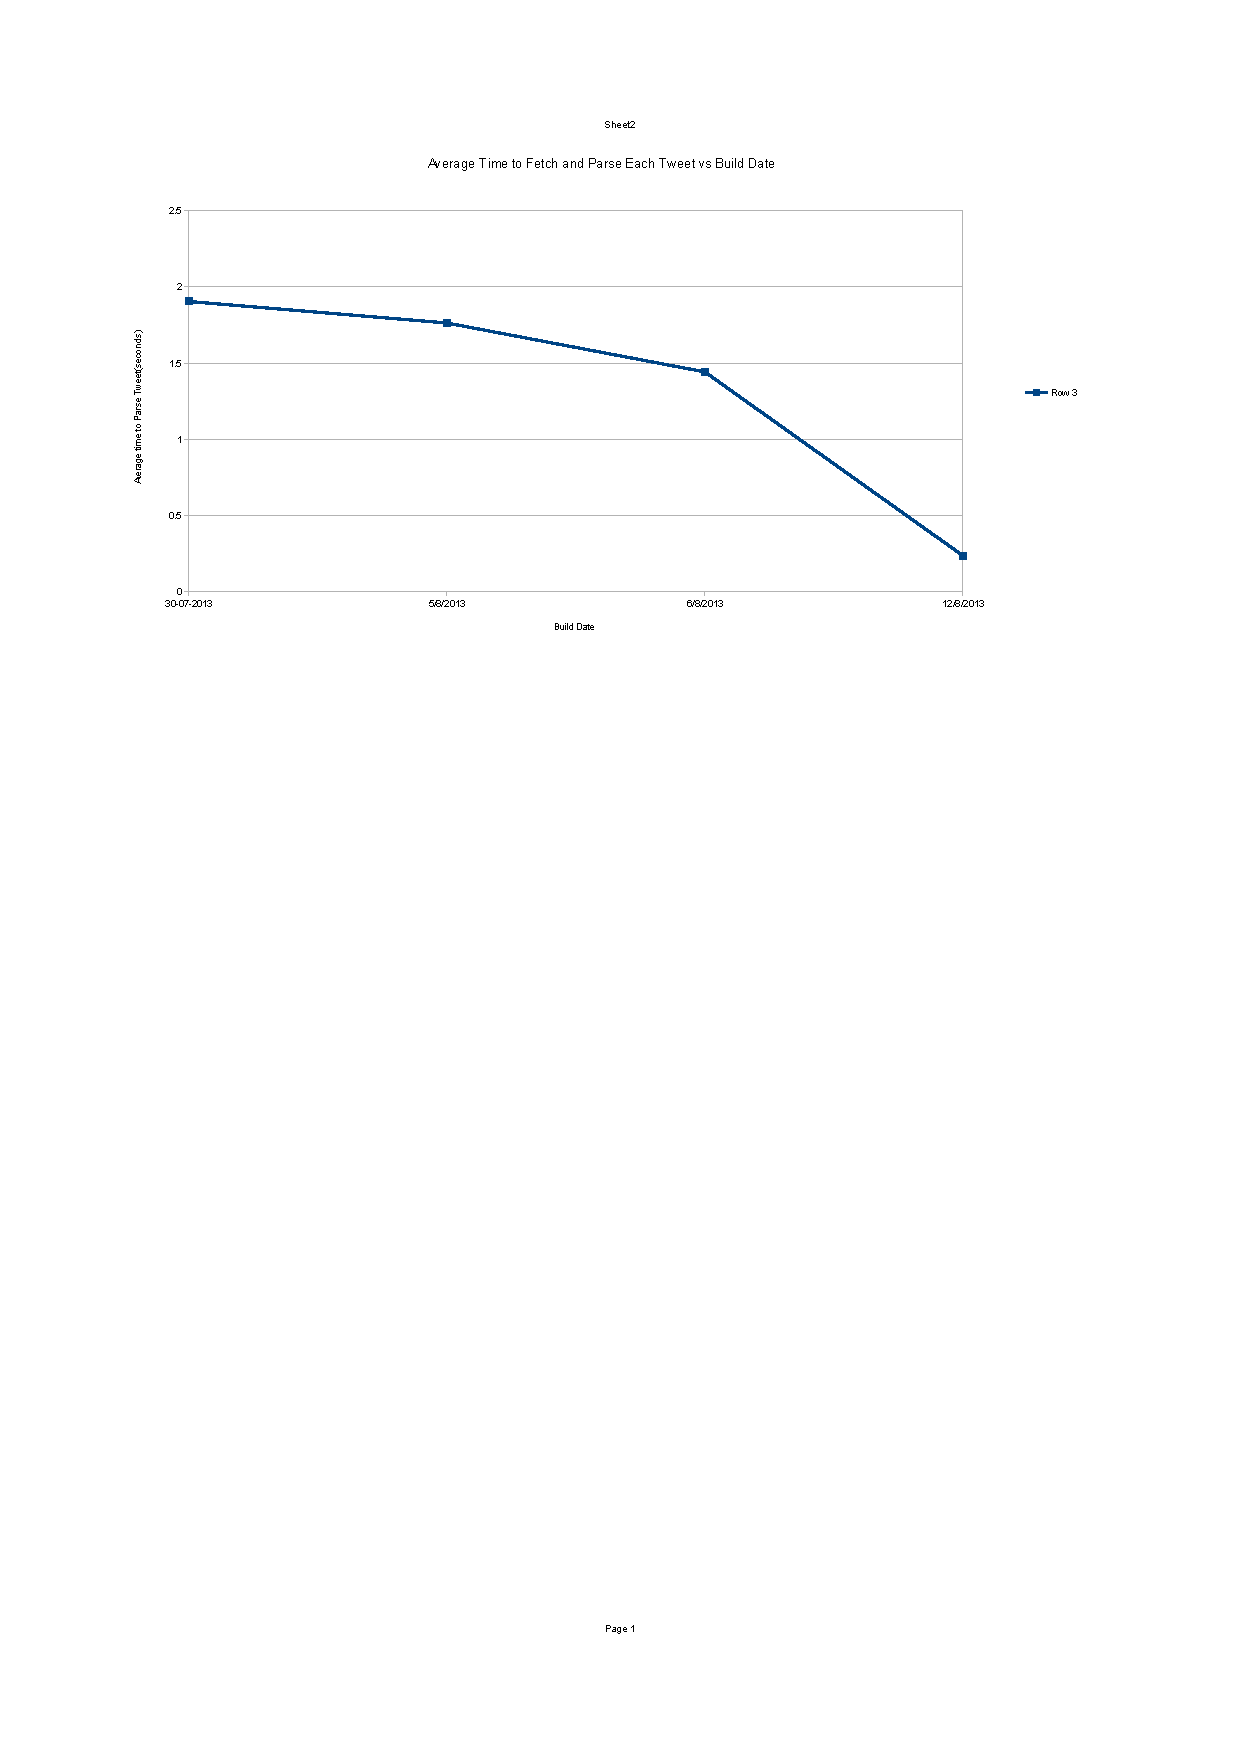
\includegraphics{Images/average_time_to_fetch_parse_tweets_per_build.pdf}
\caption{The Average Time to Fetch and Parse a Tweet, Ordered by Builds}
\end{figure}

Absolute limitations - Every tweet has to be fetched in an individual http request. This produces upper limits as to how fast the scraper can go, and means that the majority of performance speed is reliant on the speed of the network. (data - show how on some days tweets are fetched slightly faster than on other days. Times of day.)

Sensitivity of tweets fetched - it isn't actually much faster if I bulk-collect tweets in a larger 'window', as the majority of time is spent fetching the details of each tweet. 

Parellization of this? Would actually be a useful way of improving speeds...

Discuss why I did not consider parellization at the beginning. The number of requests may be too many and result in more frequent failures than otherwise. Will have to collect the data to verify this claim. 

\subsubsection{Ability to Resist Blocking Detection}

The primary measure of my scraper libraries avoiding blocking detection is with regards to their failure or incomplete-scrape rates. Although in early, less stable builds I had parsing errors, my later work only failed when detected by twitter and blocked. As such detection rates in later builds can reliably be calculated by analysing failing or incomplete twitter profiles. 

\begin{figure}[h!]
\centering
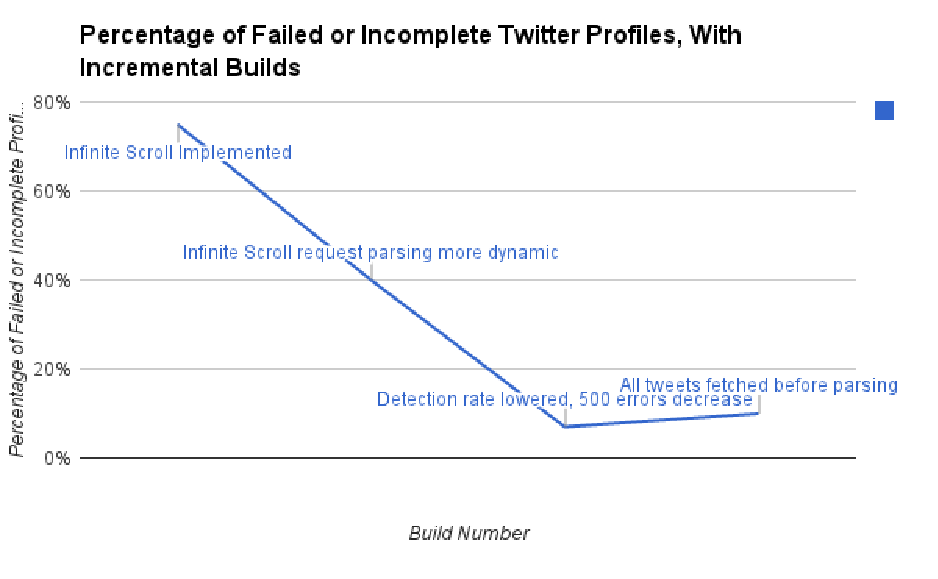
\includegraphics{Images/percentage_failed_incomplete_twitter_profiles.pdf}
\caption{The Percentage of Incomplete or Failed Profile Scrapes, Ordered by Builds}
\end{figure}

\subsubsection{Privacy Protection}

Privacy protection - this is still pretty poor, saved as structured xml, data not anonymised (makes my life easier at present)... Are there things I could be doing here potentially to increase privacy for individuals that I am scraping? Document locking, or store as RDB? Since I plan on storing this info in Graft, this could be anonymised at this point. Individual profiles and what-not. 



\chapter{Conclusions and Future Work}\label{C:us}

This section summarises work completed over the project, and reflects on successes with relation to the issues identified at the beginning of the project.

% This section draws conclusions from the results of the projects and details future work that could be conducted. 

\section{Web-Scraper Implementation}

A social media web-scraping framework was developed. This framework was developed firstly for Twitter, and was extended onto LinkedIn. I was able to demonstrate how web-scraping technologies are suitable for retrieval of basic reputation metrics. Performance of the scraper was greatly increased through incremental builds, with the final build performing a factor of 6 times better than the previous one.

Unfortunately performance to fetch and parse an entire Twitter profile was shown to be too slow to prove viable in a real-time analytical system. The lower than anticipated performance was due to the dynamic nature of today's social sites, necessitating in potentially hundreds or thousands of separate requests to retrieve an entire profile. Data retrieved was shown to be accurate, withholding some elements which can remain incomplete should their size exceed the threshold selected. Detection avoidance of the framework was also evaluated to have been successful, again up until the point of 7,000 + tweets being fetched. 

\section{Data Analysis and Resulting Policies}

Data analysis was performed against the Twitter dataset collected of 1.7 million tweets. Retweets were firstly discussed, due to their greater semantic depth than the equivalent 'favourite' mechanism. Using retweet counts as a measure of impact, an 'Impact Factor' calculation is proposed, based upon the Hirsch-Index calculation. This calculation measures productivity and response values on Twitter. Combining this figure with average monthly impact gives a view of average activity, and allows for inactive users to be detected. Different bucketing sizes may be used; in this project, a month was the bucket size of choice. 

Community detection was also experimented with, and the links of retweets and follower/following relationships explored to reveal existence of sub-communities within Twitter. Unfortunately visualisation of entire retweet communities was not achieved due to limitations with the selected visualisation tool. As the MapGenerator tool is currently undergoing improvement, there is potential for improvement in this feature.

Exemplar policies were provided, with respect to the case study of a social forum. Combination of community detection, impact factor, and temporal reputation information was demonstrated to be useful in regards to access policy constructs. 

% Exemplar policies are given, with respect to the example of a social forum. 


% \noindent The evaluation of IHPScrape demonstrates that a web-scraping solution is possible for inferring basic reputation metrics, against the primary case-study of Twitter. However performance to fetch and parse an entire profile is too slow to be viable in a commercial system. The lower than expected performance is due to the dynamic nature of today's social sites, necessitating in potentially hundreds or thousands of separate HTTP requests being sent to fetch an entire profile. 

% However the performance of policies operating on a subset of the full detail from a user's profile is significantly closer to the target aims. Whilst still not achieving response times on the order of a few seconds, when using a subset of tweets greater performance could be achieved with little information loss. Policy effectiveness resulting from data analysis strategies were varying. While the proposed impact factor and temporal clustering methods are possible with the current tools and data, community detection was more limited. The existing visualisation tool cannot handle millions of nodes and even more edges, in this case twitter profiles and their links. However the MapEquation team have acknowledged the deficiencies of their tool, and are working to port this to a non-Flash based system without such limitations. 

% Through qualitative results, retrieved data was shown to be accurate for information such as retweets, favourites and so on. Requirement R6 stated that data should not be missing or incorrect, and this was achieved in the majority of cases. When data was missing, this was due to scrapers being detected and an incomplete list of tweets being returned, for example. Design decisions had to also be made to allow for reasonable performance, such as not fetching the entire list of names who retweeted a post. 

% The framework was shown to be extensible through the implementation of a second social scraper for LinkedIn. The pattern of creating separate classes for pages and defining functions to handle data retrieval related to these pages, and abstracting the actual fetching details was easily extendible to LinkedIn, with the resulting scraper implemented in significantly less time than the original Twitter artefact and framework. I acknowledge however that the comparison is not entirely even, as LinkedIn did not have complications such as Infinite Scrolling. 

% IHPScrape was successful in avoiding detection by sites, and was never blocked entirely running on the University environment. Incomplete profiles dropped below one in ten by the final build. Recovery from detection was not implemented however, as there was no way to distinguish for example the actual end of an individual's twitter page, and the server taking action against a scraper.

% IHPScrape did not fully meet the requirement of remaining flexible despite interface change. The solution had to rely on certain xPath expressions and backend URLs remaining constant, and quantitatively evaluating the exact resistance of the scrapers to change proved infeasible within the timeframe of the project. 

% Experiences with scraping from various social sites lead to conclusions about the suitability of sites for scraping. The more dynamic a site, the more complex and unreliable data fetching will become. 

% Conclusions on which sites are suitable for scraping.


\section{Future Work}

\subsection{Community Detection Extension}

In its current state, the community detection component of my project only detects community patterns and is not able to associate meaning with these various communities. In order to support a richer set of reputation-defining policies, some form of sentiment or classification of profiles within these communities would be required. In order for more meaningful visualisation of such results, the MapGenerator tool will need to have advanced to a capable level for handling larger amounts of data. As such this was left to future work.

Further, small-world network analysis could be compared to communities detected within Twitter, and my dataset. 

\subsection{Social Media Expansion}

In order to further validate the scraping framework constructed, more social media sites should be explored. This would enable richer still policies and data analysis to be performed. Not all sites would be suitable for scraping, and indeed in some cases the API may be of more use. Sites with more static content are more suitable for web scraping. 

%Highly dynamic sites such as Facebook proved infeasible for the scraper design; but networks like Slashdot could be more suitable. 

%Compare detected embedded social networks against small-world networks and check for correlation. 

%Improve community detection elements, perhaps with sentiment or other detection methods in order to classify profiles.

\subsection{Further Evaluation}

Further verification of IHPScrape with respect to resistance to change is required. No Twitter user interface changes were experienced during the course of the project. For the scraper to be applied as part of a legitimate reputation system, verification of its resistance to interface change must be conducted. Comparison against API changes would be more valuable still.

\subsection{Reliability Metric}

Requirement F5 stated that a metric of reliability should be developed based upon quantity of data collected. The performance of policies demonstrated that fetching a full profile for use is not feasible within a real-time system. As such using only a subset of profile data could be more practical, with the attachment of some form of metric pointing to the reliability of data collected.

\subsection{GRAft integration}

As analysis components and policies developed effectively act as a source node in the GRAft model, actual implementation of this could be useful. Community effort would be required to maintain such a solution.
%\chapter{22/08/2013 Week}\label{C:us}

\section{Progress}

Got lots more data, scrapers running since Monday (couldn't do earlier due QUAKE!!!). LinkedIn scraper is now functioning, but currently broken because I started adding multi-threading. This shouldn't take long at all to fix. 

\subsection{LinkedIn}
Things I can fetch from publicly-viewable pages: 

\begin{itemize}
 \item number of connections
 \item Number of recommendations
 \item Current Position (creepy?)
 \item Number of skills listed (Often maxed out at 50)
 \item Number of groups/societies that the person has listed
\end{itemize}

\noindent Some of these could be useful/interesting to look at while others might not be (e.g. number of skills, this can just be spammed out.) Could maybe look at relationships between number of skills v recommendations, connections v recommendations.\\

\noindent It's interesting how straightforward pages such as LinkedIn are to scrape vs ones like Twitter or Facebook. Whereas twitter has some dynamic content (e.g. sepearate http request to load detailed tweet data, infinite scroll) which were challenging and time-consuming to make robust, LinkedIn does not. This is another thing I can talk about in report, some form of recommendations about easily-scrapable web pages. It seems obvious now, but it was not obvious when I was starting x many months ago. 

\section{Policies -Data Fetching!!}

Since Monday, scraped lots more profiles... ~600 were collected into this for analysis, but I have done ~800 total. These are more accurate scrapes than previous versions, given a silly bug including tweets that were actually not originally from the author in past results. So I cannot reliably use data from old scrapes too much. That's OK though - performance is much much better now. 

\subsection{Correlation of Impact Factor vs Bucketed Impacts}

\begin{figure}[h!]
\centering
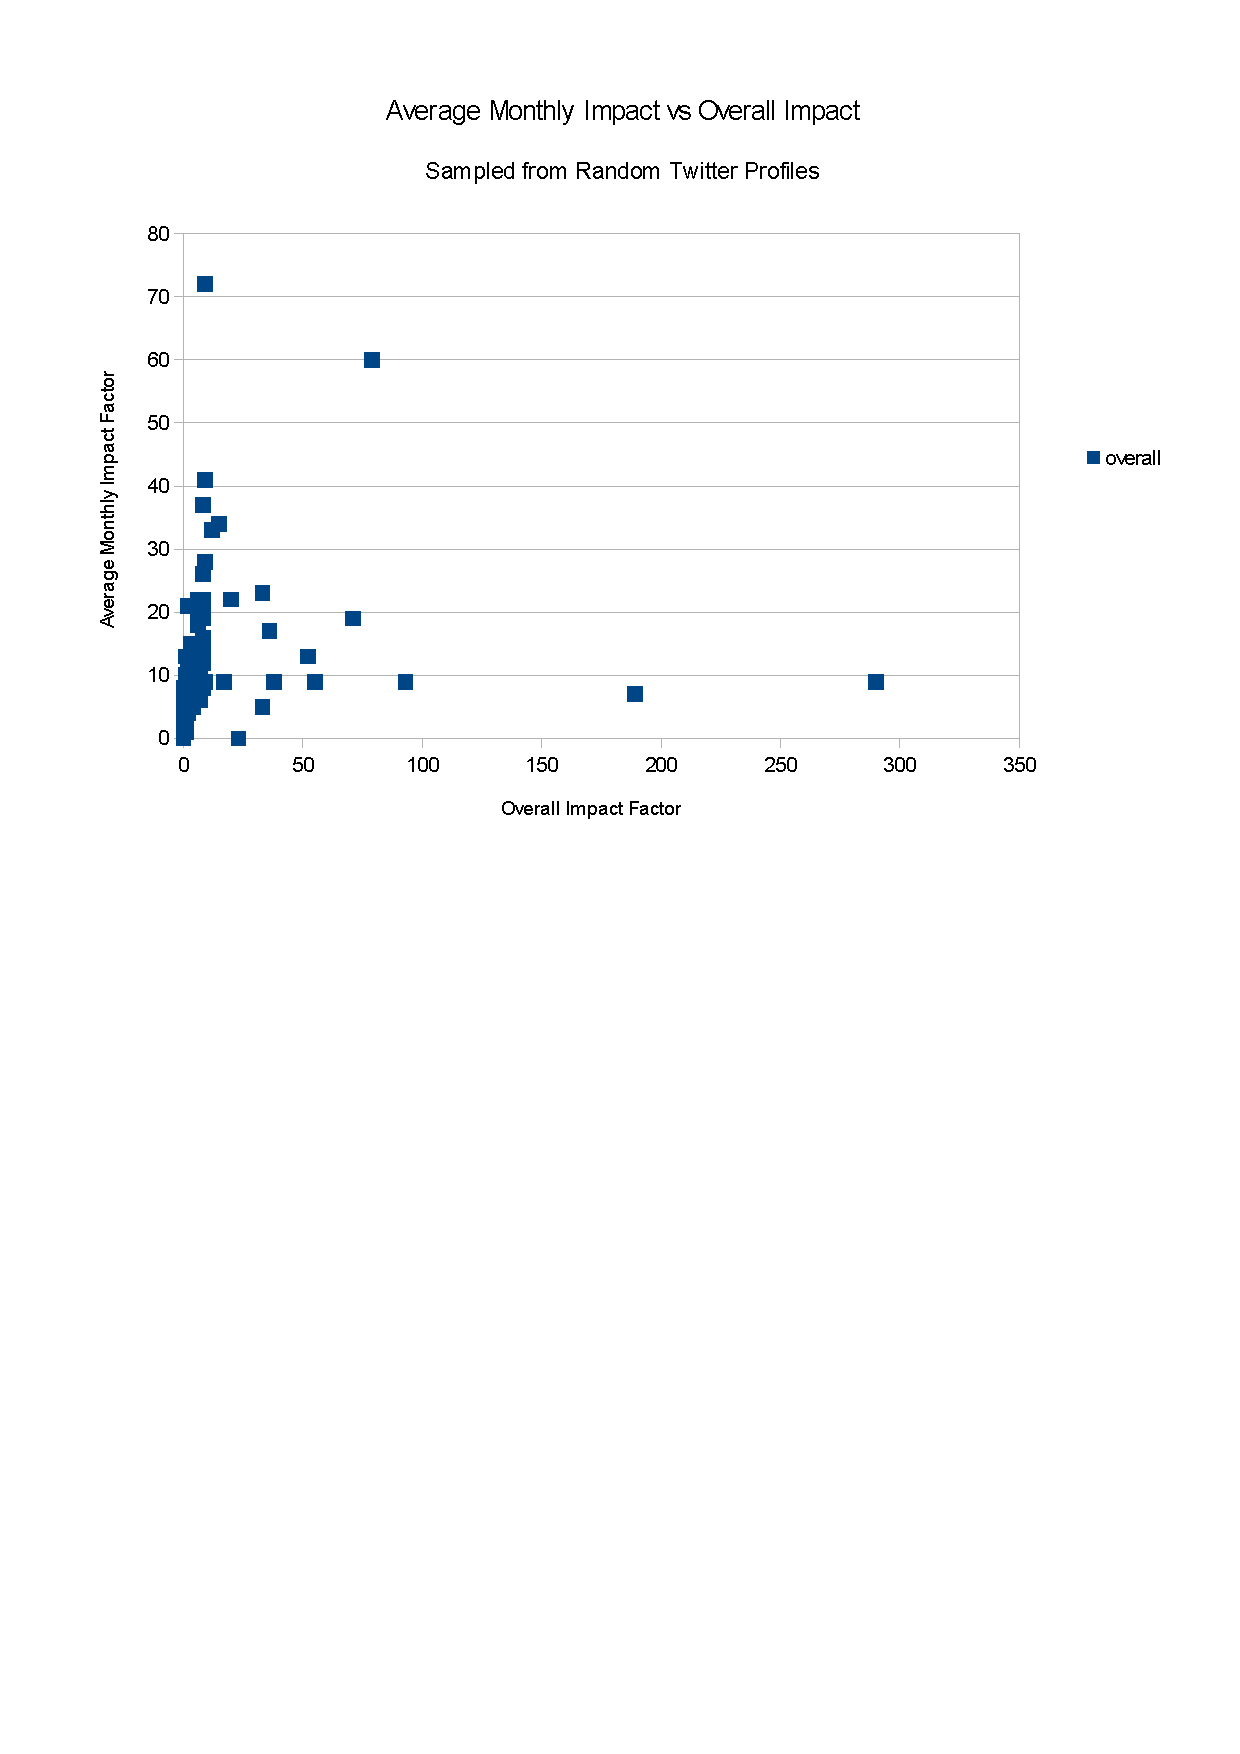
\includegraphics[width=400px]{Images/monthly_impact_vs_overallv2.pdf}
\caption{Monthly Impact against Overall Impact}
\end{figure}

\begin{figure}[h!]
\centering
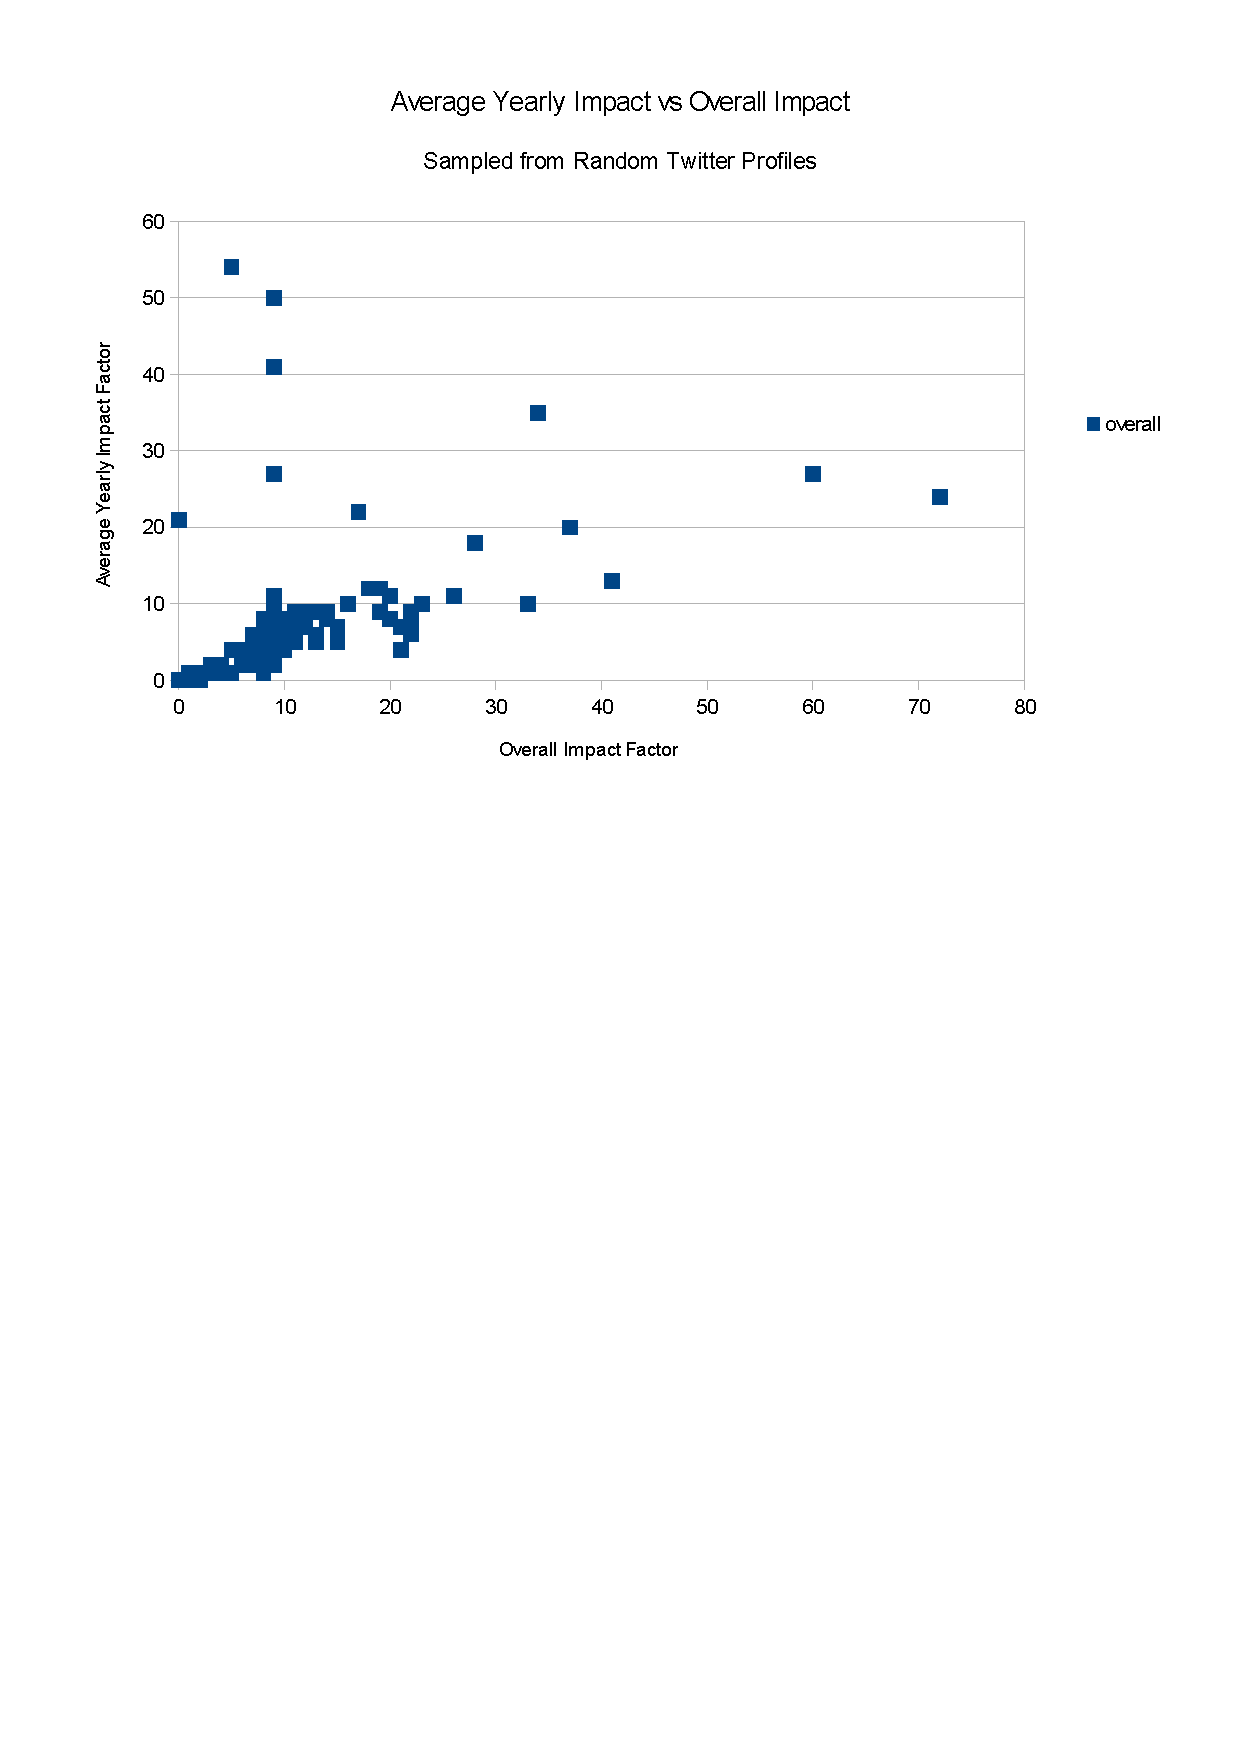
\includegraphics[width=400px]{Images/yearly_impact_vs_overallv2.pdf}
\caption{Yearly Impact against Overall Impact}
\end{figure}

One strategy for inferring reputation information that I looked at was through temporal bucketing of impact factor, into days, months, and years. The figures below show the relationship between people's mean monthly calculated impact factor (i.e. by calculating a person's impact score for each month, and then averaging these values over the total number of months), and the individual's overall impact score. I infer that there is a weak relationship between average monthly impact and overall impact (Pearson's correlation coefficient r= 0.273(3 s.f.)), and a stronger relationship between average yearly impact and overall impact (r=0.689(3 s.f.))\\

\noindent What I believe this data shows is that the impact factor is favourable to individuals who are consistent on Twitter over time. <- Need to back this up

\subsection{Results of Monthly Bucketing}

By applying the impact factor formula to individuals on a monthly basis, we are able to generate an impression of how regularly active a person is. The data also reveals how influential the person has been per month. This assists when comparing individuals who are consistently strongly influential (e.g. Barack Obama, companies such as instagram), with those who are popular for a limited period only. I looked at comparing different bucket sizes for this temporal aggregation. Days, months, and years were used as buckets, with monthly aggregation clearly showing the strongest and more interesting trends. 

\subsubsection{Twitter Scraper Performance}
I evaluate the performance of my twitter scraper with respect to average time taken to fetch and parse a tweet. The major limiting factor for scraping twitter was that each tweet had to be fetched with a seperate http request. Figure <x> shows the average time taken to fetch and parse each tweet, with respect to my incremental build stages. The success of continuous and incremental improvement in performance helps justify my decision to use an incremental approach. Tweets were gathered over several days, and continuously throughout different times of the day on the Victoria network to ensure that a representative range of times were gathered for each stage.\\

\noindent The significant feature of improved performance was through parellization of tweet-fetches. 

\begin{figure}[h!]
\centering
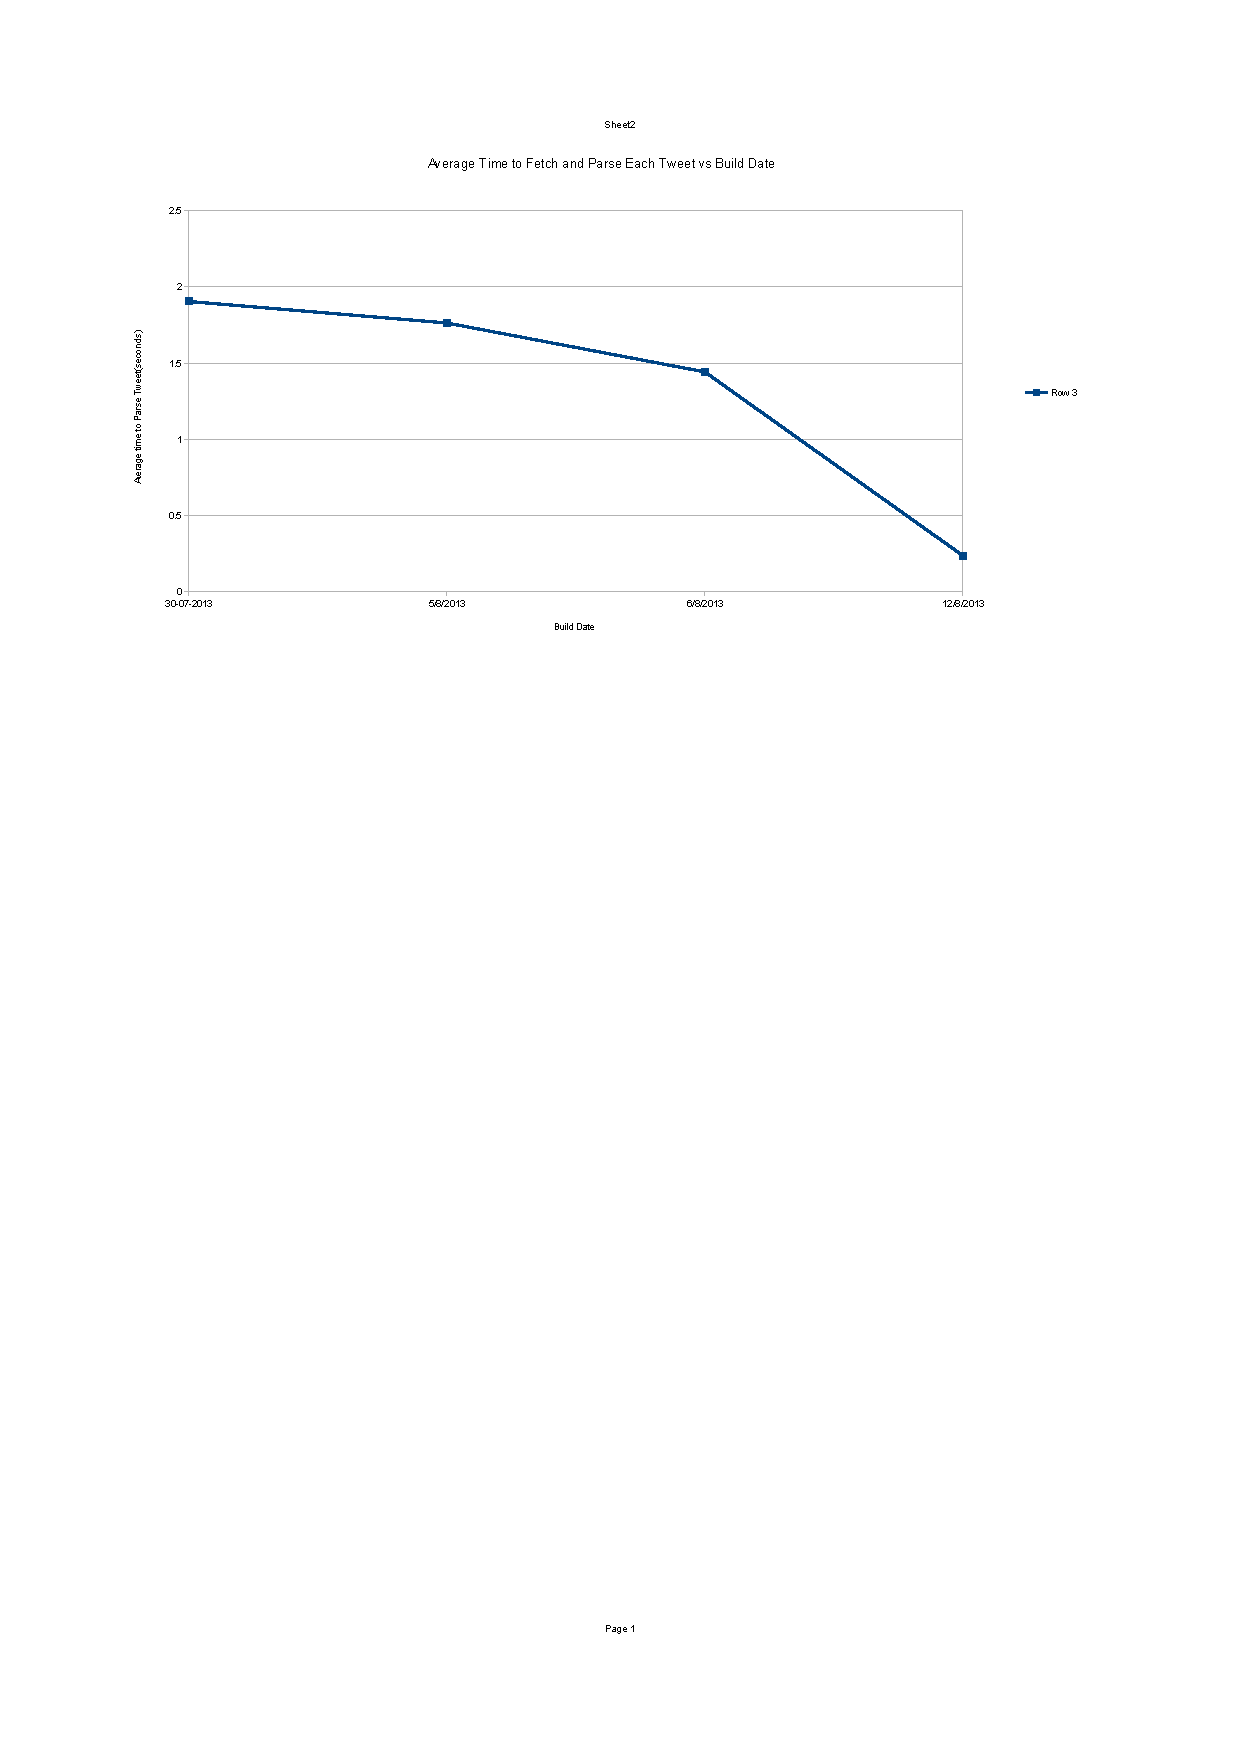
\includegraphics{Images/average_time_to_fetch_parse_tweets_per_build.pdf}
\caption{The Average Time to Fetch and Parse a Tweet, Ordered by Builds}
\end{figure}

Absolute limitations - Every tweet has to be fetched in an individual http request. This produces upper limits as to how fast the scraper can go, and means that the majority of performance speed is reliant on the speed of the network. (data - show how on some days tweets are fetched slightly faster than on other days. Times of day.)


\subsubsection{Ability to Resist Blocking Detection}

The primary measure of my scraper libraries avoiding blocking detection is with regards to their failure or incomplete-scrape rates. Although in early, less stable builds I had parsing errors, my later work only failed when detected by twitter and blocked. As such detection rates in later builds can reliably be calculated by analysing failing or incomplete twitter profiles. 

\begin{figure}[h!]
\centering
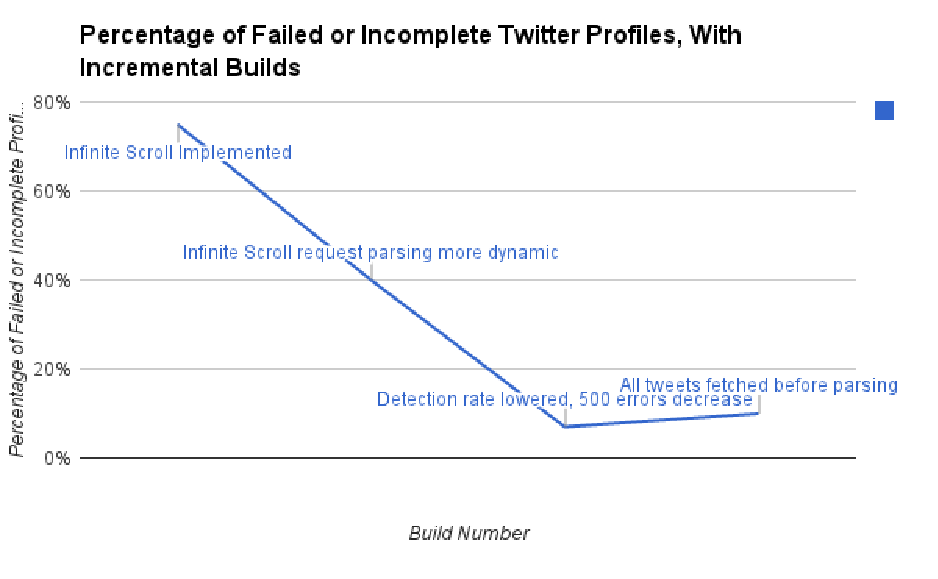
\includegraphics{Images/percentage_failed_incomplete_twitter_profiles.pdf}
\caption{The Percentage of Incomplete or Failed Profile Scrapes, Ordered by Builds}
\end{figure}

\subsubsection{Privacy Protection}

Privacy protection - this is still pretty poor, saved as structured xml, data not anonymised (makes my life easier at present)... Are there things I could be doing here potentially to increase privacy for individuals that I am scraping? Document locking, or store as RDB? Although storage into GRAft would require community effort/a business model and is therefore unlikely, it might add value to my report to demonstrate how this would be feasible through better privacy measures. 



%%%%%%%%%%%%%%%%%%%%%%%%%%%%%%%%%%%%%%%%%%%%%%%%%%%%%%%

\backmatter

%%%%%%%%%%%%%%%%%%%%%%%%%%%%%%%%%%%%%%%%%%%%%%%%%%%%%%%


%\bibliographystyle{ieeetr}
\nocite{*}
\bibliographystyle{acm}
\bibliography{bibliography}


\end{document}
